\part{Part 3: Applications}

\graphicspath{ {./Pictures/} }
\chapterimage{chapter_head_2.pdf} % Chapter heading image

%++++++++++++++++++++++++++++++++++++++++++++++++++++++++++++++
\chapter{Introduction}
\label{ch:intro for tutorials}
%++++++++++++++++++++++++++++++++++++++++++++++++++++++++++++++
\section{Gmsh}
\begin{gmshnote}
	To read all about Gmsh and download its source, executables, and license please \href{http://gmsh.info}{\underline{click here}}.
\end{gmshnote}
Gmsh is an 2D/3D mesh generator including a built-in CAD engine and post-processor. Gmsh was developed to provide a fast, lightweight, and user-friendly meshing environment with additional visualization capabilities. It is open source, and the source code and executables for various operating systems (Windows, Mac, Linux) are available for free. Gmsh contains modules for geometry definition, meshing, solving and post-processing. Each module has its own set of commands and utilities, which can be easily manipulated using a graphical user-interface (GUI).

Upon launching the Gmsh executable, the GUI will open and the the module panel appears on the left-hand side of the window with headings to control the:
\begin{itemize}
    \item \textbf{Geometry}
    \item \textbf{Mesh}
    \item \textbf{Solver}
\end{itemize}
The \textbf{Geometry} section is a module that allows you to create your own geometry directly within Gmsh, or import external CAD files. Geometry in Gmsh is defined using a hierarchical structure. This means a volume is made up of different surfaces, and each surface is made up of different curves or lines. In turn, each curve or line is bounded by two end points in the case of a straight line, or a sequence of points in the case of a spline, for example. Therefore, to define a desired geometry a set of points are specified first, and the connections between these points are built using straight lines or curves. Then, a set of surfaces are created using the lines and curves, which are themselves used to define a volume in the case of a three-dimensional problem.

The geometry module has some key features to allow you to accomplish these tasks. Some of the important features are:
\begin{itemize}
    \item \textbf{Elementary entities}: Create, merge, split or delete points, lines, curves, faces or volumes.
    \item \textbf{Physical groups}: Specify boundary conditions and physical properties of a particular geometric entity.
    \item \textbf{Reload script}: Re-read the geometry saved in your .geo file, the Gmsh native file format.
    \item \textbf{Edit script}: Edit the .geo file manually using a built-in text editor.
\end{itemize}
It is worth noting that geometry specifications are saved in the .geo file in plain text format. This allows you to manually manipulate your geometry or any other specifications by editing this file using either the in-built text editor, or an external one of your choice. 

After building the geometry and defining the boundary conditions via the \textbf{Geometry} module, the next step is usually to generate a mesh of the geometry using the \textbf{Mesh} module. This module splits the geometry up into a number of simple geometric elements, such as: lines, triangles, tetrahedra, hexahedra and pyramids. Gmsh has several different algorithms for automatically generating a mesh, and an unstructured mesh will be generated by default. The \textbf{Mesh} module has sections that help to specify the type, number, and density of the mesh in the computational domain. Some of the important sections are:
\begin{itemize}
    \item \textbf{Define}: Set the number of points and stretching ratios along lines. Additionally, control the mesh type (whether structured or unstructured).
    \item \textbf{2D/3D}: Generates the mesh for surfaces/volumes in the domain. It automatically generates the mesh using specifications provided in the \textbf{Define} section.
\end{itemize}
There is another module named \textbf{Solver}, which allows a numerical solver to be accessed directly from within Gmsh. In the context of the current book, this will not be used.

\section{SU2}
\begin{su2note}
	To read all about SU2 and download its source, executables, and license please \href{https://su2code.github.io/}{\underline{click here}}.
\end{su2note}
As discussed in the Physics and Numerics parts of this book, ultimately an approximate solution to the Navier-Stokes or RANS equations is obtained by solving a discrete system of equations on a computational grid, or mesh. SU2 is an open-source CFD solver built specifically for this task. SU2 is written in C++, and its primary applications are computational aerodynamics and shape optimization. SU2 is generally user-friendly, and pre-compiled versions are available for all major operating systems (Windows, Mac, Linux). In the following tutorials we will demonstrate the utility of SU2 as a CFD tool for computational aerodynamics.

%++++++++++++++++++++++++++++++++++++++++++++++++++++++++++++++
\section{Paraview}
\begin{paraviewnote}
	To read all about Paraview and download its source, executables, and license please \href{https://www.paraview.org/}{\underline{click here}}.
\end{paraviewnote}
After SU2 runs it generates a set of data files, which includes the complete flow field solved on the mesh generated previously using Gmsh. This data must be post-processed to visualize flow structures of interest, such as the velocity or pressure fields. Paraview is an open-source and multi-platform visualization package designed for this task. It is also available for all operating systems (Windows, Mac, Linux) and is free to download and use. Paraview is designed specifically to handle large complex data sets, such as those generated in CFD simulations. In the following laboratory experiments, we will use Paraview as a post-processing tool for the analysis of the data produced by SU2. Typically, this analysis consists of contours of flow parameters, extracting line plots, slices, or pressure coefficient distributions.

%++++++++++++++++++++++++++++++++++++++++++++++++++++++++++++++
\chapter{Inviscid NACA 0012}
\label{ch:Inviscid NACA 0012}
%++++++++++++++++++++++++++++++++++++++++++++++++++++++++++++++
\section{Required Files}
\begin{su2note}
	Use the following links to download the same version of SU2 for Windows (\href{https://users.encs.concordia.ca/~bvermeir/book/executables/windows/SU2-v7.0.0-win64.zip}{\underline{click here}}) or Mac (\href{https://users.encs.concordia.ca/~bvermeir/book/executables/osx/SU2-v7.0.0-macos64.zip}{\underline{click here}}), and the required configuration (\href{https://gitlab.com/bvermeir/book-cfd/blob/master/tutorial/tut1_inviscid_NACA 0012/inv_NACA 0012.cfg}{\underline{click here}}) and mesh files (\href{https://gitlab.com/bvermeir/book-cfd/blob/master/tutorial/tut1_inviscid_NACA 0012/mesh_NACA 0012_inv.su2}{\underline{click here}}).
\end{su2note}
\begin{paraviewnote}
	Use the following links to download the same version of Paraview for Windows (\href{https://users.encs.concordia.ca/~bvermeir/book/executables/windows/ParaView-5.4.0-Qt5-OpenGL2-Windows-64bit.exe}{\underline{click here}}) or Mac (\href{https://users.encs.concordia.ca/~bvermeir/book/executables/osx/ParaView-5.4.0-Qt5-OpenGL2-MPI-OSX10.8-64bit.dmg}{\underline{click here}}).
\end{paraviewnote}

\section{Problem Description}
In this tutorial we are going to demonstrate how to simulate transonic inviscid flow around a NACA 0012 airfoil. Under the assumption of inviscid flow, the Euler equations will be used. Please note that this assumption is only reasonably valid at high Reynolds numbers and low angles of attack, since the contribution of the viscous terms in the Navier-Stokes equations is minimal in this case. The flow specifications are provided as:
\begin{itemize}
    \item Pressure = 101,325 Pa
    \item Temperature = 273 K
    \item Mach number = 0.8
    \item Angle of attack = 1.25 degree
\end{itemize}
This tutorial has two parts: Flow Solution and Post-Processing. In the first part we will explain how to manage the required files and settings in SU2, and then run the simulation. In the second part we will demonstrate how to use Paraview to visualize the data files generated in the first step using SU2.
%++++++++++++++++++++++++++++++++++++++++++++++++++++++++++++++
\section{Flow solution}
To run this simulation SU2 needs two files: a configuration file (.cfg) and a mesh file (.su2). Links to the required files and executables are provided at the start of this tutorial. The files include:
\begin{enumerate}
\item \textit{inv\_NACA 0012}.cfg: the configuration file.
\item \textit{mesh\_NACA 0012\_inv}.su2: the mesh file.
\end{enumerate}
The next step is to copy these two files in the directory you have save the SU2 executable, so everything is located in the same folder. Then, to run the simulation using the executable, mesh, and configuration files simply open a terminal window and enter the following commands:
\begin{table}[htbp]
    \centering
    \begin{tabular}{|l|l|}
    \hline
    Windows     & \begin{tabular}{c} \$ cd "where you saved the package" \\ \$ SU2\_CFD.exe inv\_NACA 0012.cfg \end{tabular}
    \\
    \hline
    Mac     & \begin{tabular}{c} \$ cd "where you saved the package" \\ \$ SU2\_CFD.exe inv\_NACA 0012.cfg \end{tabular}
    \\
    \hline
    \end{tabular}
\end{table}

The SU2 solver will commence solving the problem and will print out the residuals at every iteration, until the specified convergence criteria is achieved. After the calculations are complete the following output files should have been generated within in the SU2 folder:
\begin{itemize}
    \item \textit{flow}.vtk: The flow solution on the entire domain.
    \item \textit{force\_breakdown}.dat: Forces and moment on the airfoil.
    \item \textit{history}.vtk: Convergence history.
    \item \textit{restart\_flow}.dat: Restart file.
    \item \textit{surface\_flow}.vtk: The flow solution on the airfoil surface.
    \item \textit{surface\_flow}.csv: A comma separated value file of the flow solution on the airfoil.
\end{itemize}
Please keep in mind that every time you run SU2, the output data will be overwritten. Hence, before launching a new simulation you should backup your files in another directory.
%++++++++++++++++++++++++++++++++++++++++++++++++++++++++++++++
\section{Post-Processing}
In this section we will explain how to use Paraview to visualize the solution files generated by SU2. First of all, install Paraview using the links at the start of this tutorial. Once that is complete, perform the following steps to visualize the results:
%--------------------------------------------------------------
\subsection{Open the Solution:}
Launch Paraview. Go to \textbf{File} $\rightarrow$ \textbf{Open}, and then select the \textit{flow}.vtk file. On the left-hand side of the Paraview window you will see the file appear under \textbf{builtin} in the \textbf{Pipeline Browser}. Now press the \textbf{Apply} button in the \textbf{Properties} tab, right under the \textbf{Pipeline Browser} heading. After taking these steps, your file is loaded by Paraview and is ready to be visualized (Figure \ref{fig1:load}).
\begin{figure}[htbp]
    \centering
    \includegraphics[width=0.4\textwidth]{tut01/loadvtkfile.pdf}
    \caption{Loading the .vtk file into the \textbf{Pipeline Browser}.}
    \label{fig1:load}
\end{figure}
%--------------------------------------------------------------
\subsection{Visualize the Mesh}
In order to view the mesh that was stored in the .su2 file, and as shown in Figure \ref{fig1:wireframe}, select \textit{Solid Color} with \textit{Wireframe} in the toolbar. Then, you can zoom in to see the mesh near the surface of the airfoil, as shown in Figure \ref{fig1:mesh}. The mesh around the NACA 0012 is unstructured, and the elements are clustered around the leading and trailing edges to resolve the complex flow structures that are expected there.
\begin{figure}[htbp]
    \centering
    \includegraphics[width=0.6\textwidth]{tut01/wireframe.pdf}
    \caption{Displaying the NACA 0012 mesh.}
    \label{fig1:wireframe}
\end{figure}
\begin{figure}[htbp]
    \centering
    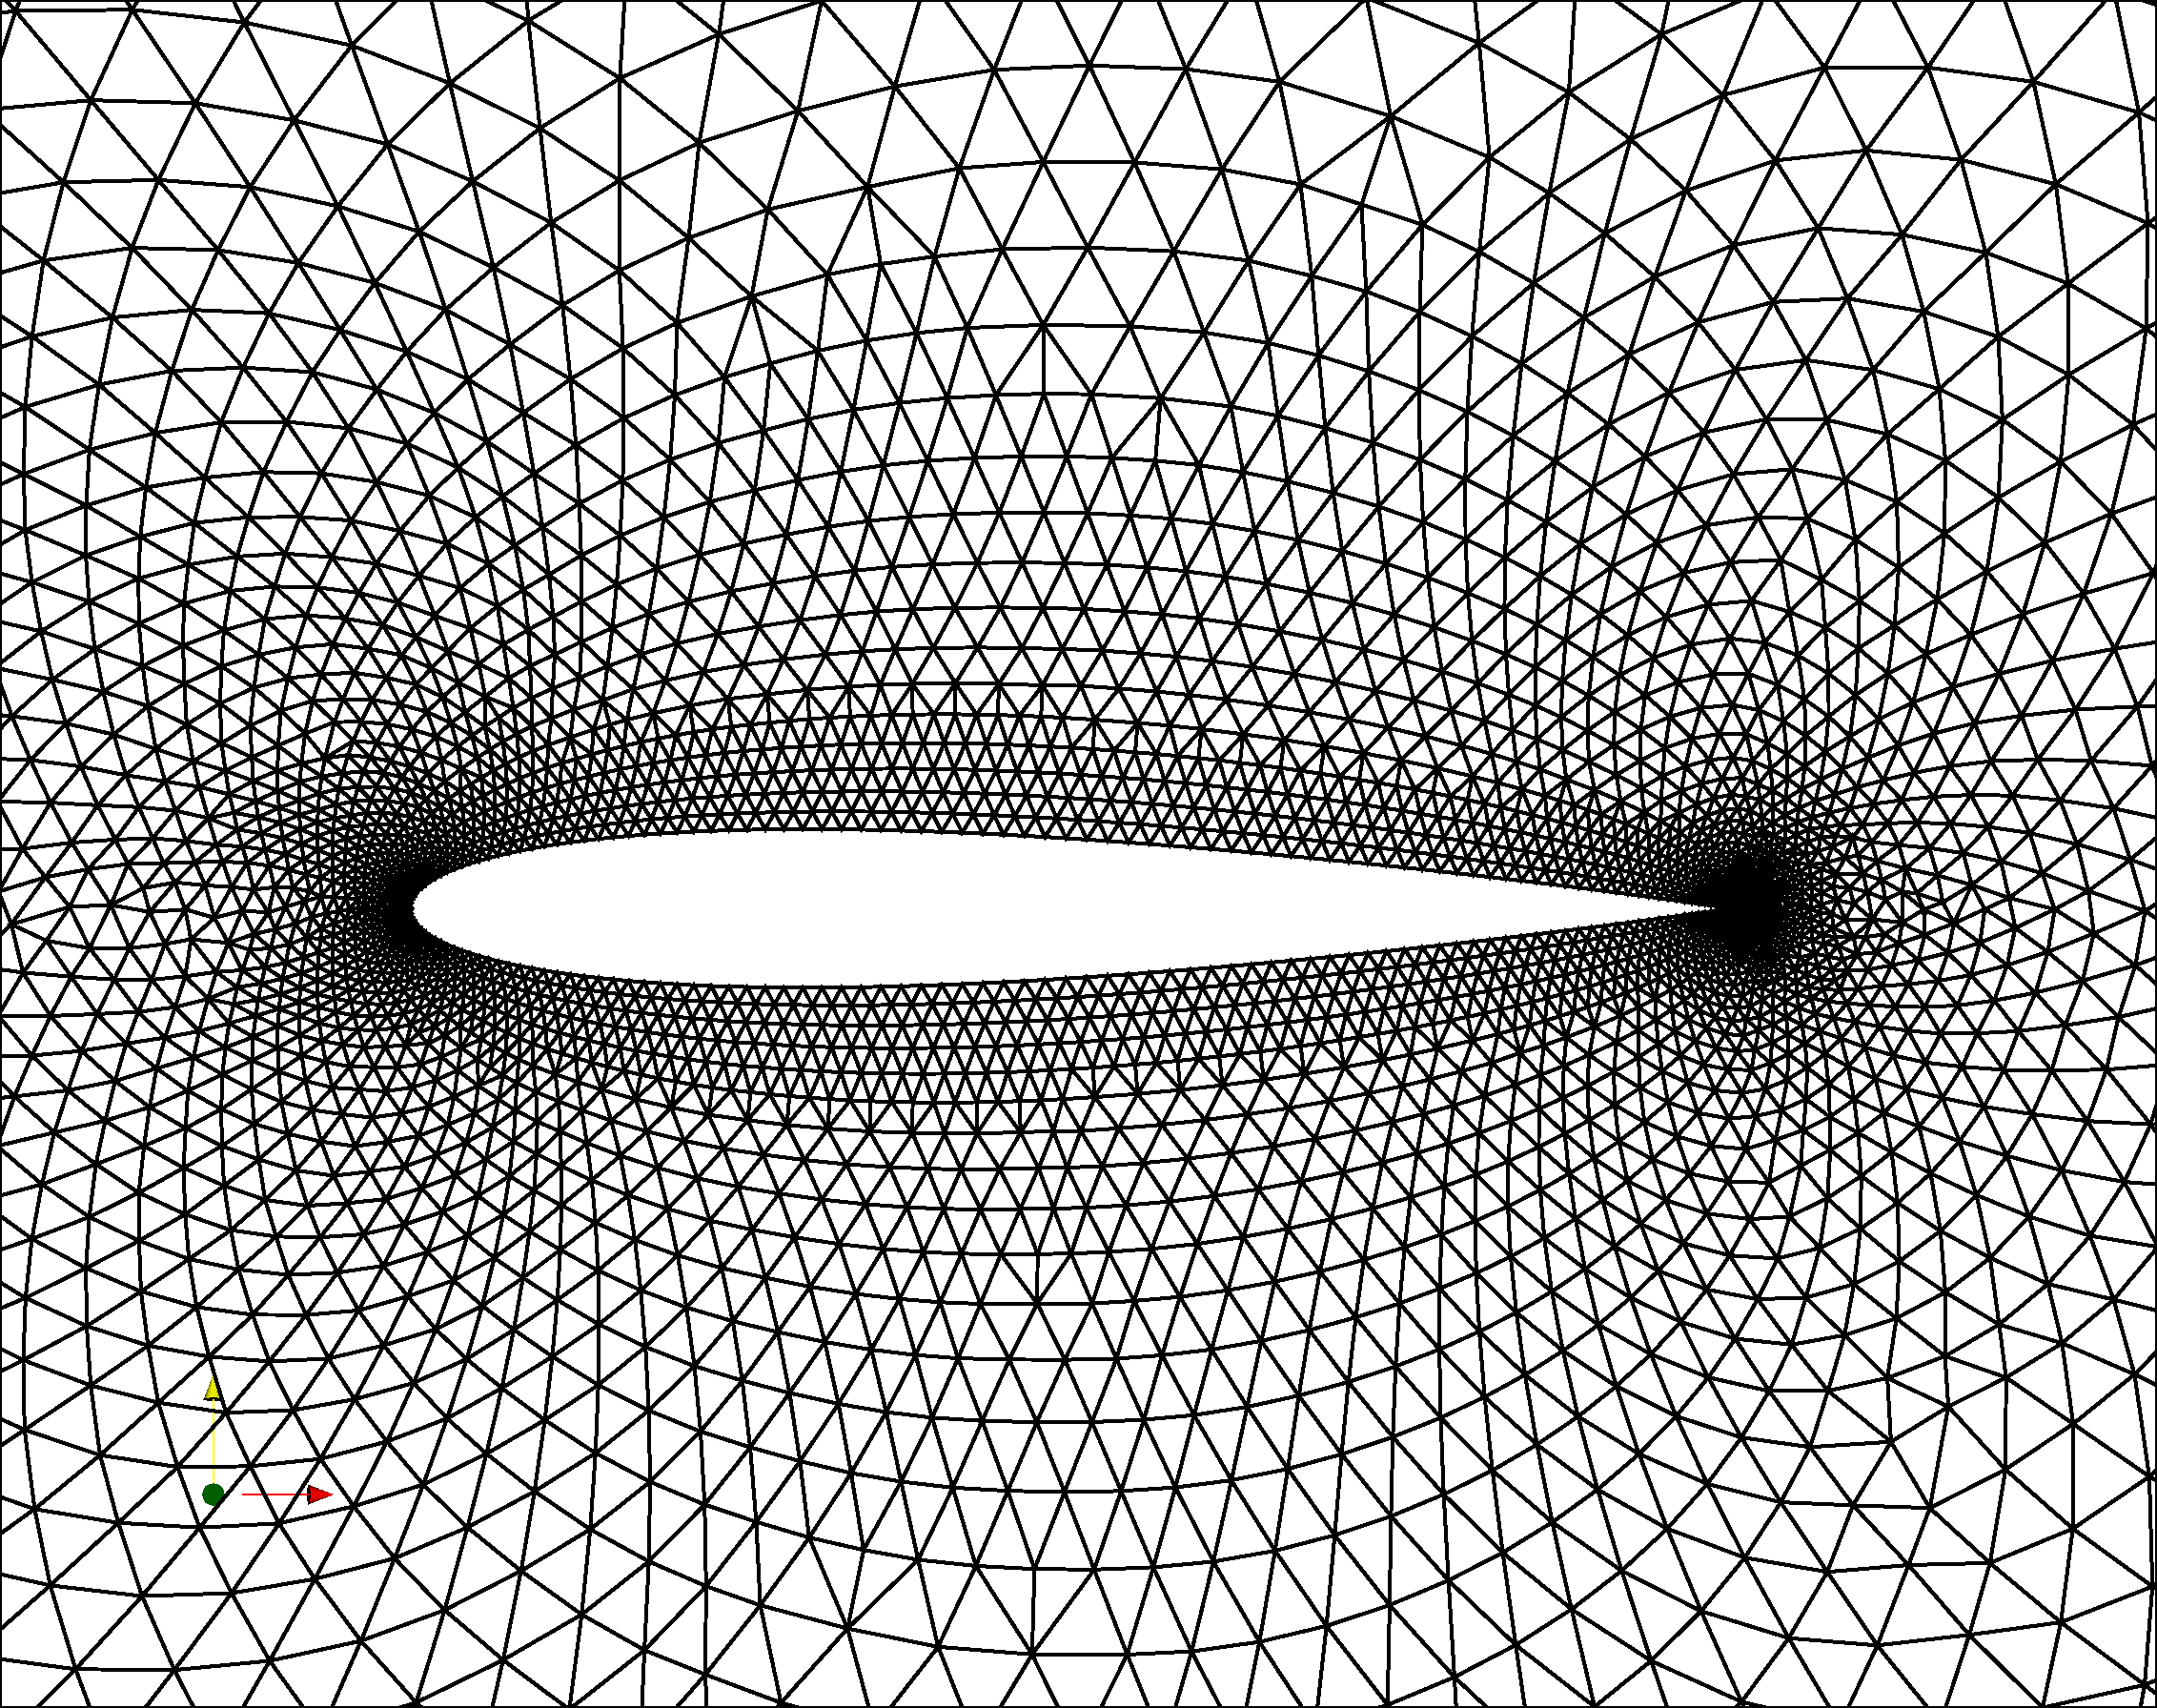
\includegraphics[width=.75\textwidth]{tut01/mesh.pdf}
    \caption{The unstructured mesh around the NACA 0012 airfoil.}
    \label{fig1:mesh}
\end{figure}
%--------------------------------------------------------------
\subsection{Visualize Pressure Contours}
In order to visualize pressure contours click on \textit{flow}.vtk from within the \textbf{Pipeline Browser} to select the current data file. Then click on the \textbf{Properties} tab. According to Figure \ref{fig1:colorby}, in the \textbf{Coloring} section select \textit{Pressure} from the drop-down menu. To change the color settings used to show the pressure field you can click on \textbf{Edit} under the \textbf{Coloring} options. Another display window appears on the right-hand side of the monitor, similar to Figure \ref{fig1:change_color_range}. Now you can change the maximum/minimum range of pressure to your desired values using the \textbf{Set Range} option, or change the contour colors using \textbf{Choose Preset} field (Figure \ref{fig1:change_color_range}). After these steps, the pressure contours shown in the display window should be similar to those shown in Figure \ref{fig1:pressure_contour}.
\begin{figure}[htbp]
    \centering
    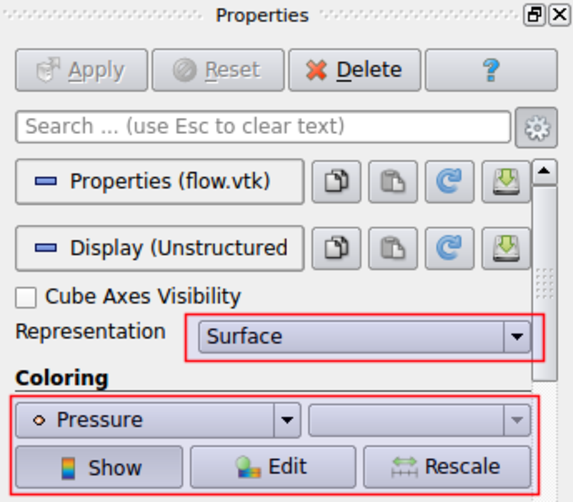
\includegraphics[width=0.4\textwidth]{tut01/contourdisplay.pdf}
    \caption{Contour settings in the \textbf{Display} tab.}
    \label{fig1:colorby}
\end{figure}
\begin{figure}[htbp]
    \centering
    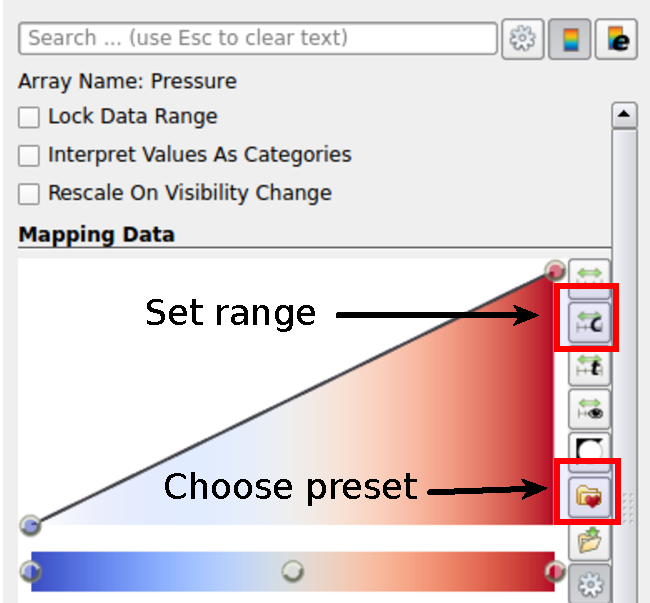
\includegraphics[width=0.5\textwidth]{tut01/colormap.pdf}
    \caption{How to change color and max/min values for contours.}
    \label{fig1:change_color_range}
\end{figure}
\begin{figure}[htbp]
    \centering
    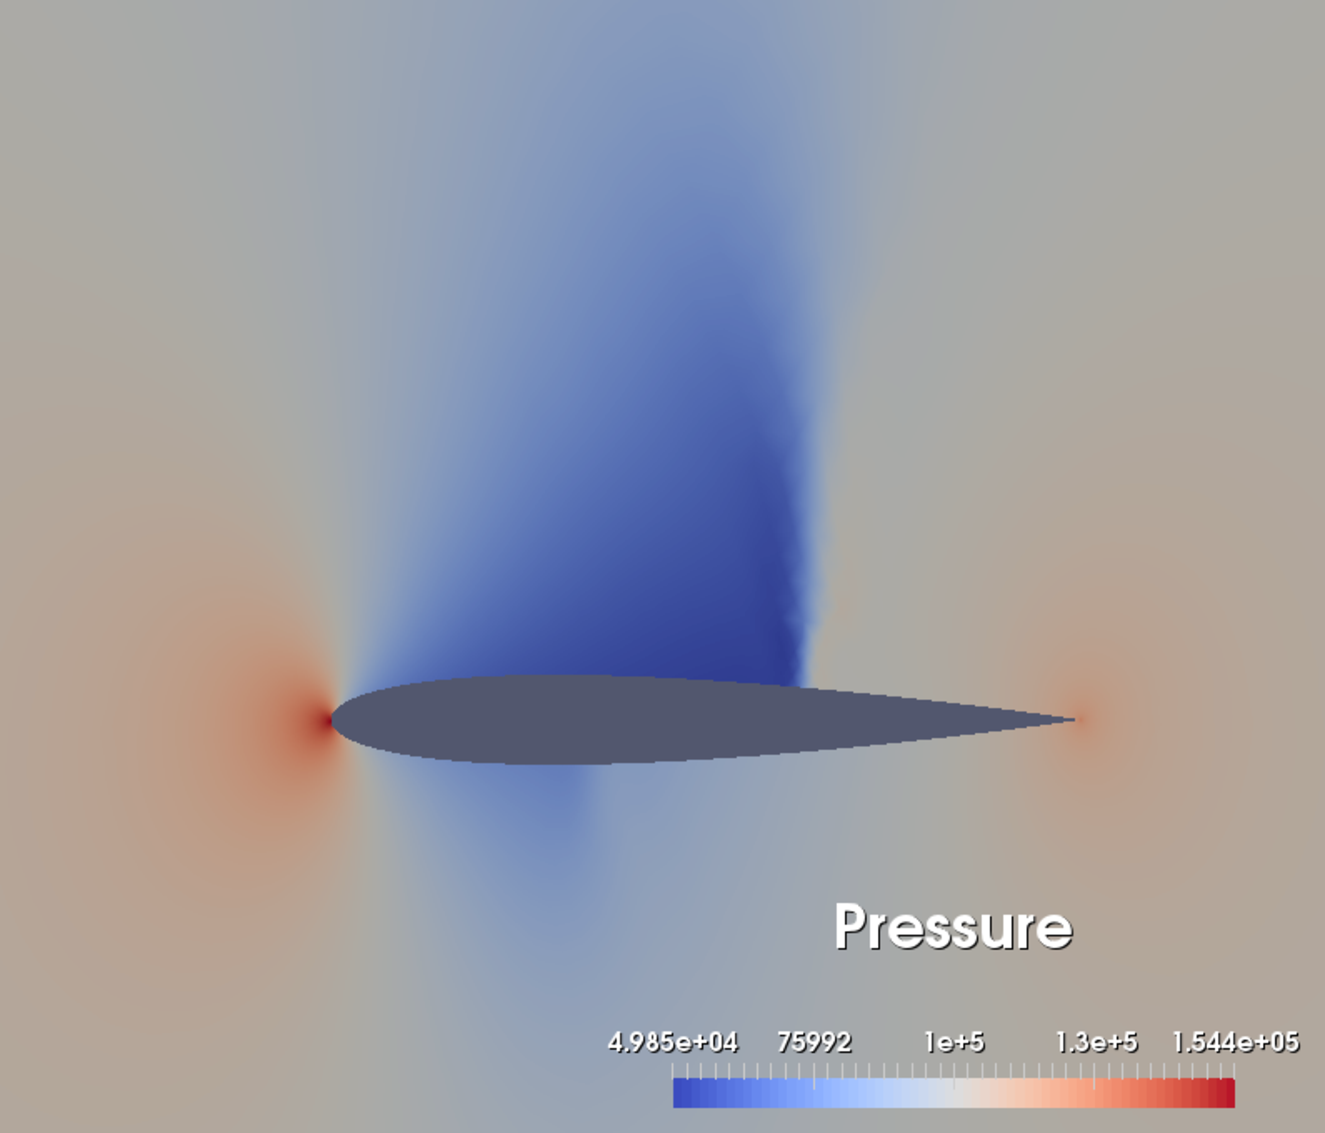
\includegraphics[width=.75\textwidth]{tut01/pressurecontour1.pdf}
    \caption{Pressure contour for NACA 0012 airfoil.}
    \label{fig1:pressure_contour}
\end{figure}

To add contour lines, click again on the \textit{flow}.vtk file in the \textbf{Pipeline Browser}, and then click on the \textbf{Contour} icon (Figure \ref{fig1:contour_icon}) in the toolbar.
\begin{figure}[htbp]
    \centering
    \includegraphics[width=0.6\textwidth]{tut01/contourlineicon.pdf}
    \caption{Contour icon in the toolbar.}
    \label{fig1:contour_icon}
\end{figure}
Now you should see that a new item called \textit{Contour1} appears under \textit{flow}.vtk in the \textbf{Pipeline Browser} (Figure \ref{fig1:contour1}).
\begin{figure}[htbp]
    \centering
    \includegraphics[width=0.5\textwidth]{tut01/contour1.pdf}
    \caption{Adding \textit{Contour1} in \textbf{Pipeline Browser}.}
    \label{fig1:contour1}
\end{figure}
As shown in Figure \ref{fig1:contourby a}, go to the \textbf{Properties} tab, and select \textit{Pressure} from the \textbf{Contour By} drop-down menu. Next, click on the \textbf{New Range} icon to customize the range of contour lines that will be generated. For now, set the number of steps to 20, similar to Figure \ref{fig1:contourby b}. This means the pressure contour range is equally divided by 20 portions between the minimum and maximum values. Finally, click on \textbf{Apply} to generate these contour lines in the display window.
\begin{figure}[htbp]
    \centering
     \begin{subfigure}[b]{.4\textwidth}
         \centering
         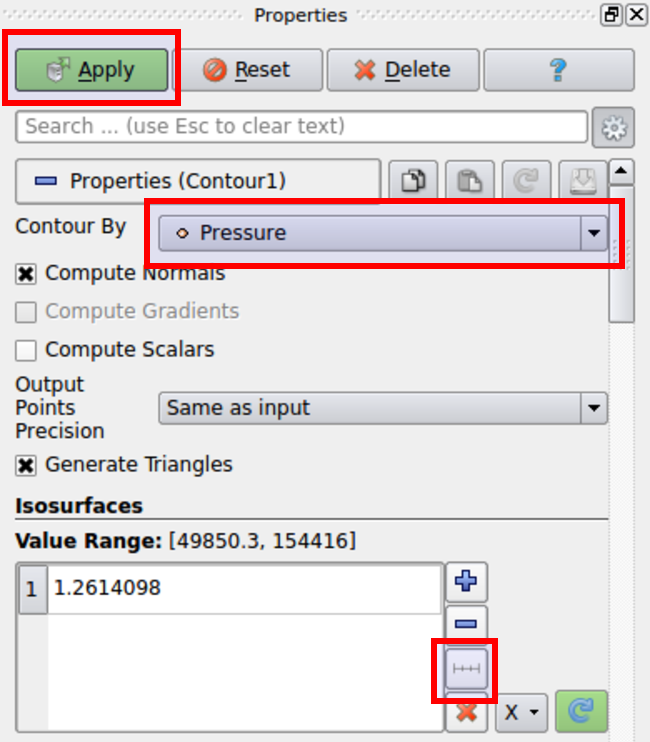
\includegraphics[width=1.0\textwidth]{tut01/contourlinenewrange.pdf}
         \caption{Define a new range}
         \label{fig1:contourby a}
     \end{subfigure}
     \hfill
     \begin{subfigure}[b]{.4\textwidth}
         \centering
         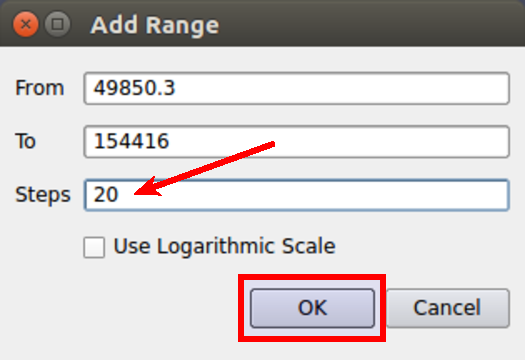
\includegraphics[width=1.0\textwidth]{tut01/addrangepdf.pdf}
         \caption{Add range}
         \label{fig1:contourby b}
     \end{subfigure}     
    \caption{How to define a new range for the contour lines.}
    \label{fig1:contourby}
\end{figure}
Next, as shown in Figure \ref{fig1:colorby2}, click on \textbf{Display} under the \textbf{Properties} tab. In the \textbf{Coloring} section, select \textbf{Solid Color} from the drop-down menu, and choose white as the color using \textbf{Edit}.
\begin{figure}[htbp]
    \centering
    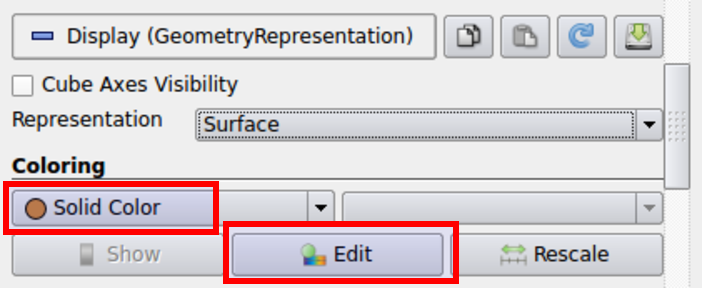
\includegraphics[width=0.6\textwidth]{tut01/coloring.pdf}
    \caption{Changing contour line colors in the \textbf{Coloring} section.}
    \label{fig1:colorby2}
\end{figure}
Now the pressure contour lines should look similar to those in Figure \ref{fig1:pressure_contour_lines}.
\begin{figure}[htbp]
    \centering
    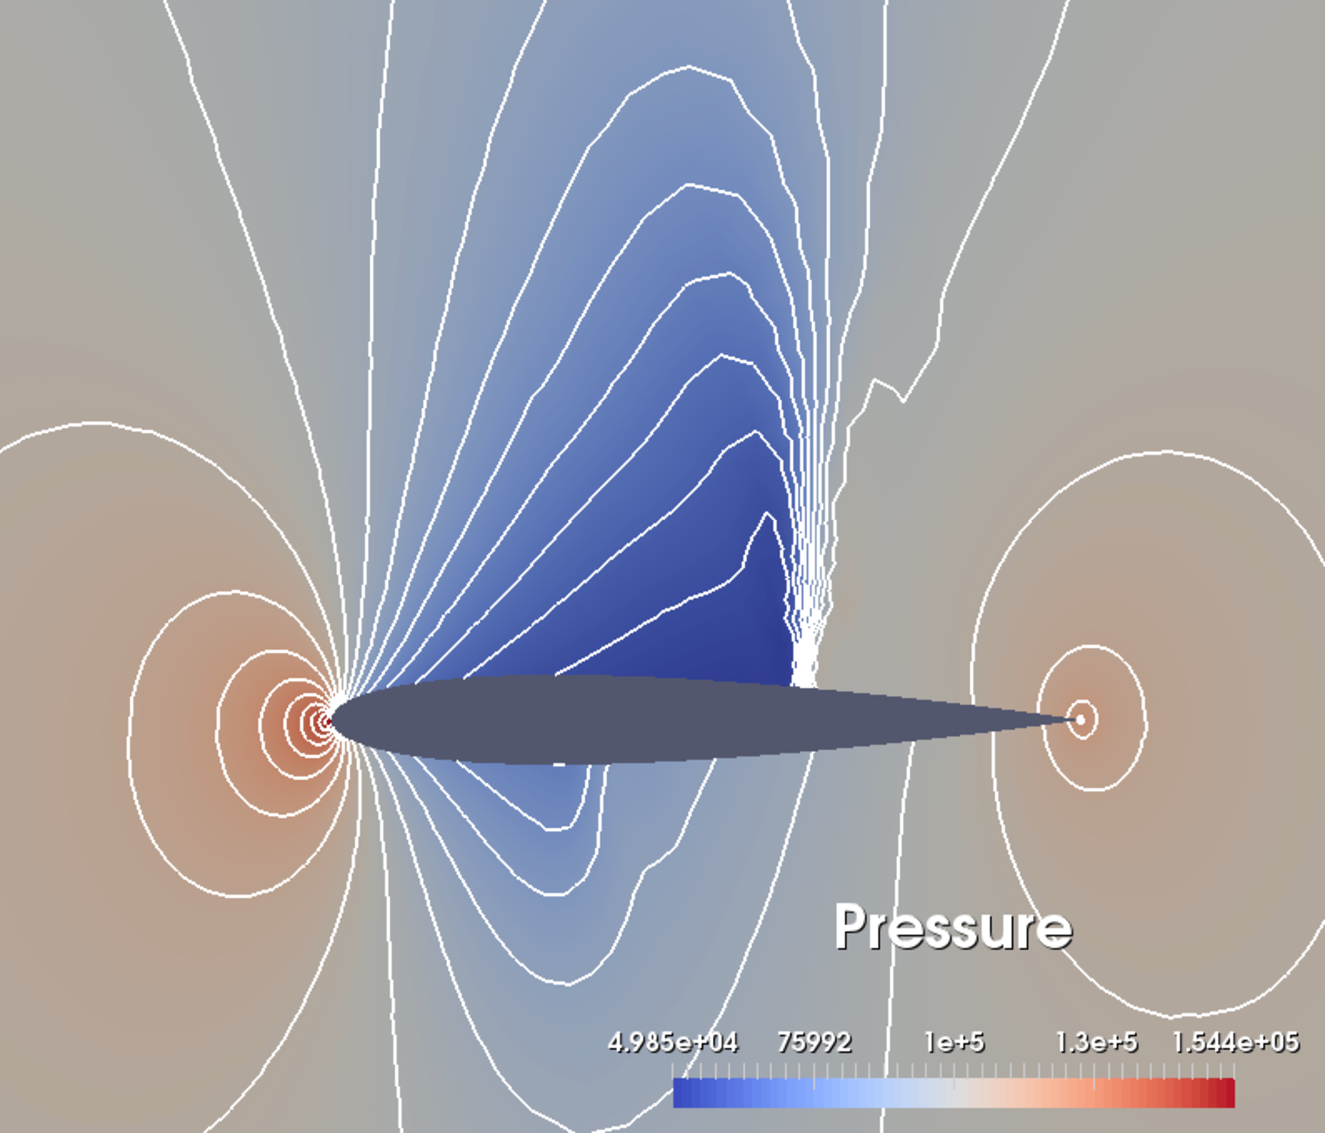
\includegraphics[width=.75\textwidth]{tut01/pressurecontour2.pdf}
    \caption{Pressure contours superimposed with contour lines around the NACA 0012 airfoil.}
    \label{fig1:pressure_contour_lines}
\end{figure}
%--------------------------------------------------------------
\subsection{Visualize the Pressure Coefficient}
The pressure data on the surface of the airfoil is stored in \textit{surface\_flow}.vtk. We will now generate a plot of the pressure coefficient as a function of chord-wise position. Go to \textbf{Open} $\rightarrow$ \textbf{File} and select \textit{surface\_flow}.vtk. As shown in Figure \ref{fig1:builtin}, this file is now loaded and added to the list of items under \textbf{builtin} in the \textbf{Pipeline Browser}.
\begin{figure}[htbp]
    \centering
    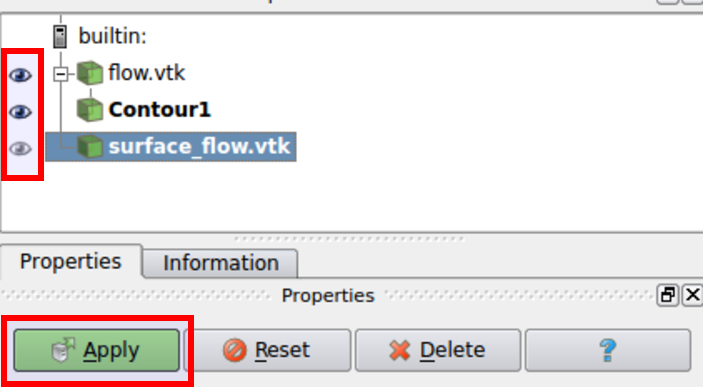
\includegraphics[width=0.5\textwidth]{tut01/eyeiconsurfaceflow.pdf}
    \caption{Loading the surface .vtk file into Paraview.}
    \label{fig1:builtin}
\end{figure}
Note that there is an eye icon on the left-hand side of each item in the \textbf{Pipeline Browser}, which enables you to hide/unhide the plots related to each item. Since we want to see only the pressure coefficient plot, we hide the previously-generated contours by unselecting the eye icon beside \textit{flow}.vtk and \textit{Contour1}. 

As shown in Figure \ref{fig1:plotdata}, select \textit{surface\_flow}.vtk in the \textbf{Pipeline Browser} and go to \textbf{Filters} $\rightarrow$ \textbf{Search} (Figure \ref{fig1:plotdata a}) and search for \textbf{Plot Data} (Figure \ref{fig1:plotdata b}). 
\begin{figure}[htbp]
    \centering
     \begin{subfigure}[b]{.4\textwidth}
         \centering
         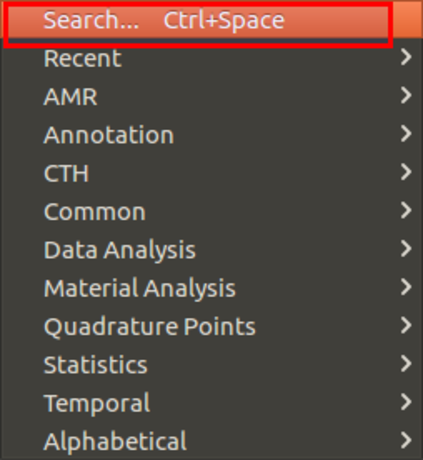
\includegraphics[width=1.0\textwidth]{tut01/filtersearch.pdf}
         \caption{Searching for a \textbf{Filter}}
         \label{fig1:plotdata a}
     \end{subfigure}
     \hfill
     \begin{subfigure}[b]{.4\textwidth}
         \centering
         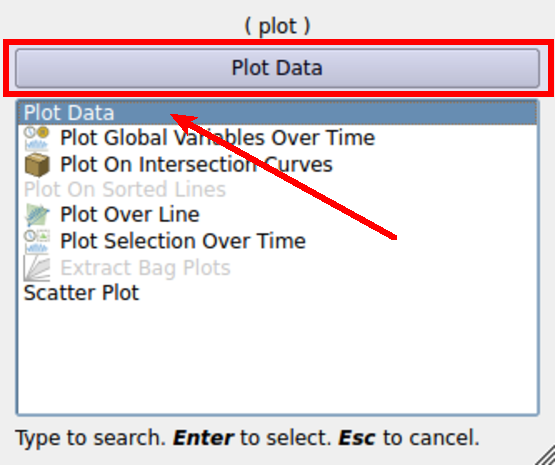
\includegraphics[width=1.0\textwidth]{tut01/plotdatasearch.pdf}
         \caption{Searching for the \textbf{PlotData} filter}
         \label{fig1:plotdata b}
     \end{subfigure}     
    \caption{How to plot data.}
    \label{fig1:plotdata}
\end{figure}

After taking this step, as shown in Figure \ref{fig1:plotdata-list}, the \textit{PlotData1} item is added to the \textbf{Pipeline Browser}. Hide (deactivate) all items in the list of the \textbf{Pipeline Browser} except \textit{PlotData1} by clicking on the eye icons beside each, and then click on \textbf{Apply}.
\begin{figure}[htbp]
    \centering
    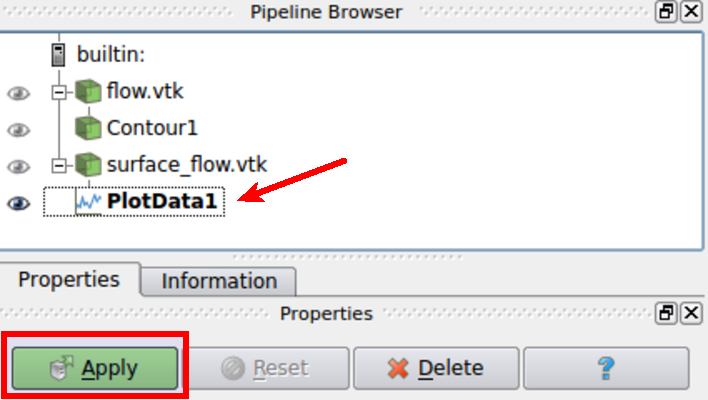
\includegraphics[width=0.5\textwidth]{tut01/plotdata1.pdf}
    \caption{Adding \textit{PlotData1} to the \textbf{Pipeline Browser}.}
    \label{fig1:plotdata-list}
\end{figure}
As shown in Figure \ref{fig1:pointsx}, under \textbf{Display} in the \textbf{Properties} tab deactivate \textbf{Use Index For XAxis}, and then select \textit{Points\_X} from the drop-down menu. 
\begin{figure}[htbp]
    \centering
    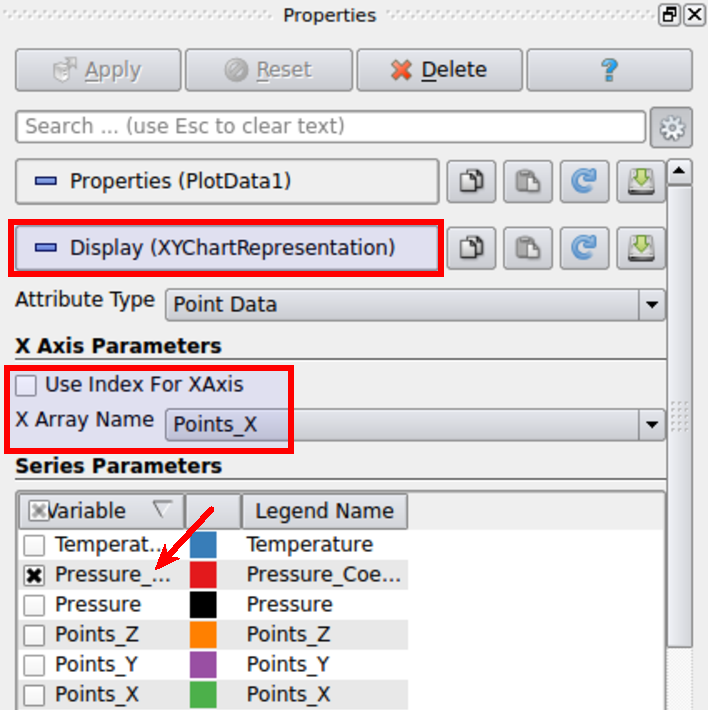
\includegraphics[width=0.5\textwidth]{tut01/plotcurvesetting.pdf}
    \caption{Plot settings for pressure coefficient along the airfoil surface.}
    \label{fig1:pointsx}
\end{figure}
Under \textbf{Series Parameters} in the same tab, unselect all variables except for \textit{Pressure\_Coefficient}. This allows you to have only one plot showing the pressure coefficient versus chord wise position. The pressure plot in the display window should be similar to that shown in Figure \ref{fig1:surface_pressure}.
\begin{figure}[htbp]
    \centering
    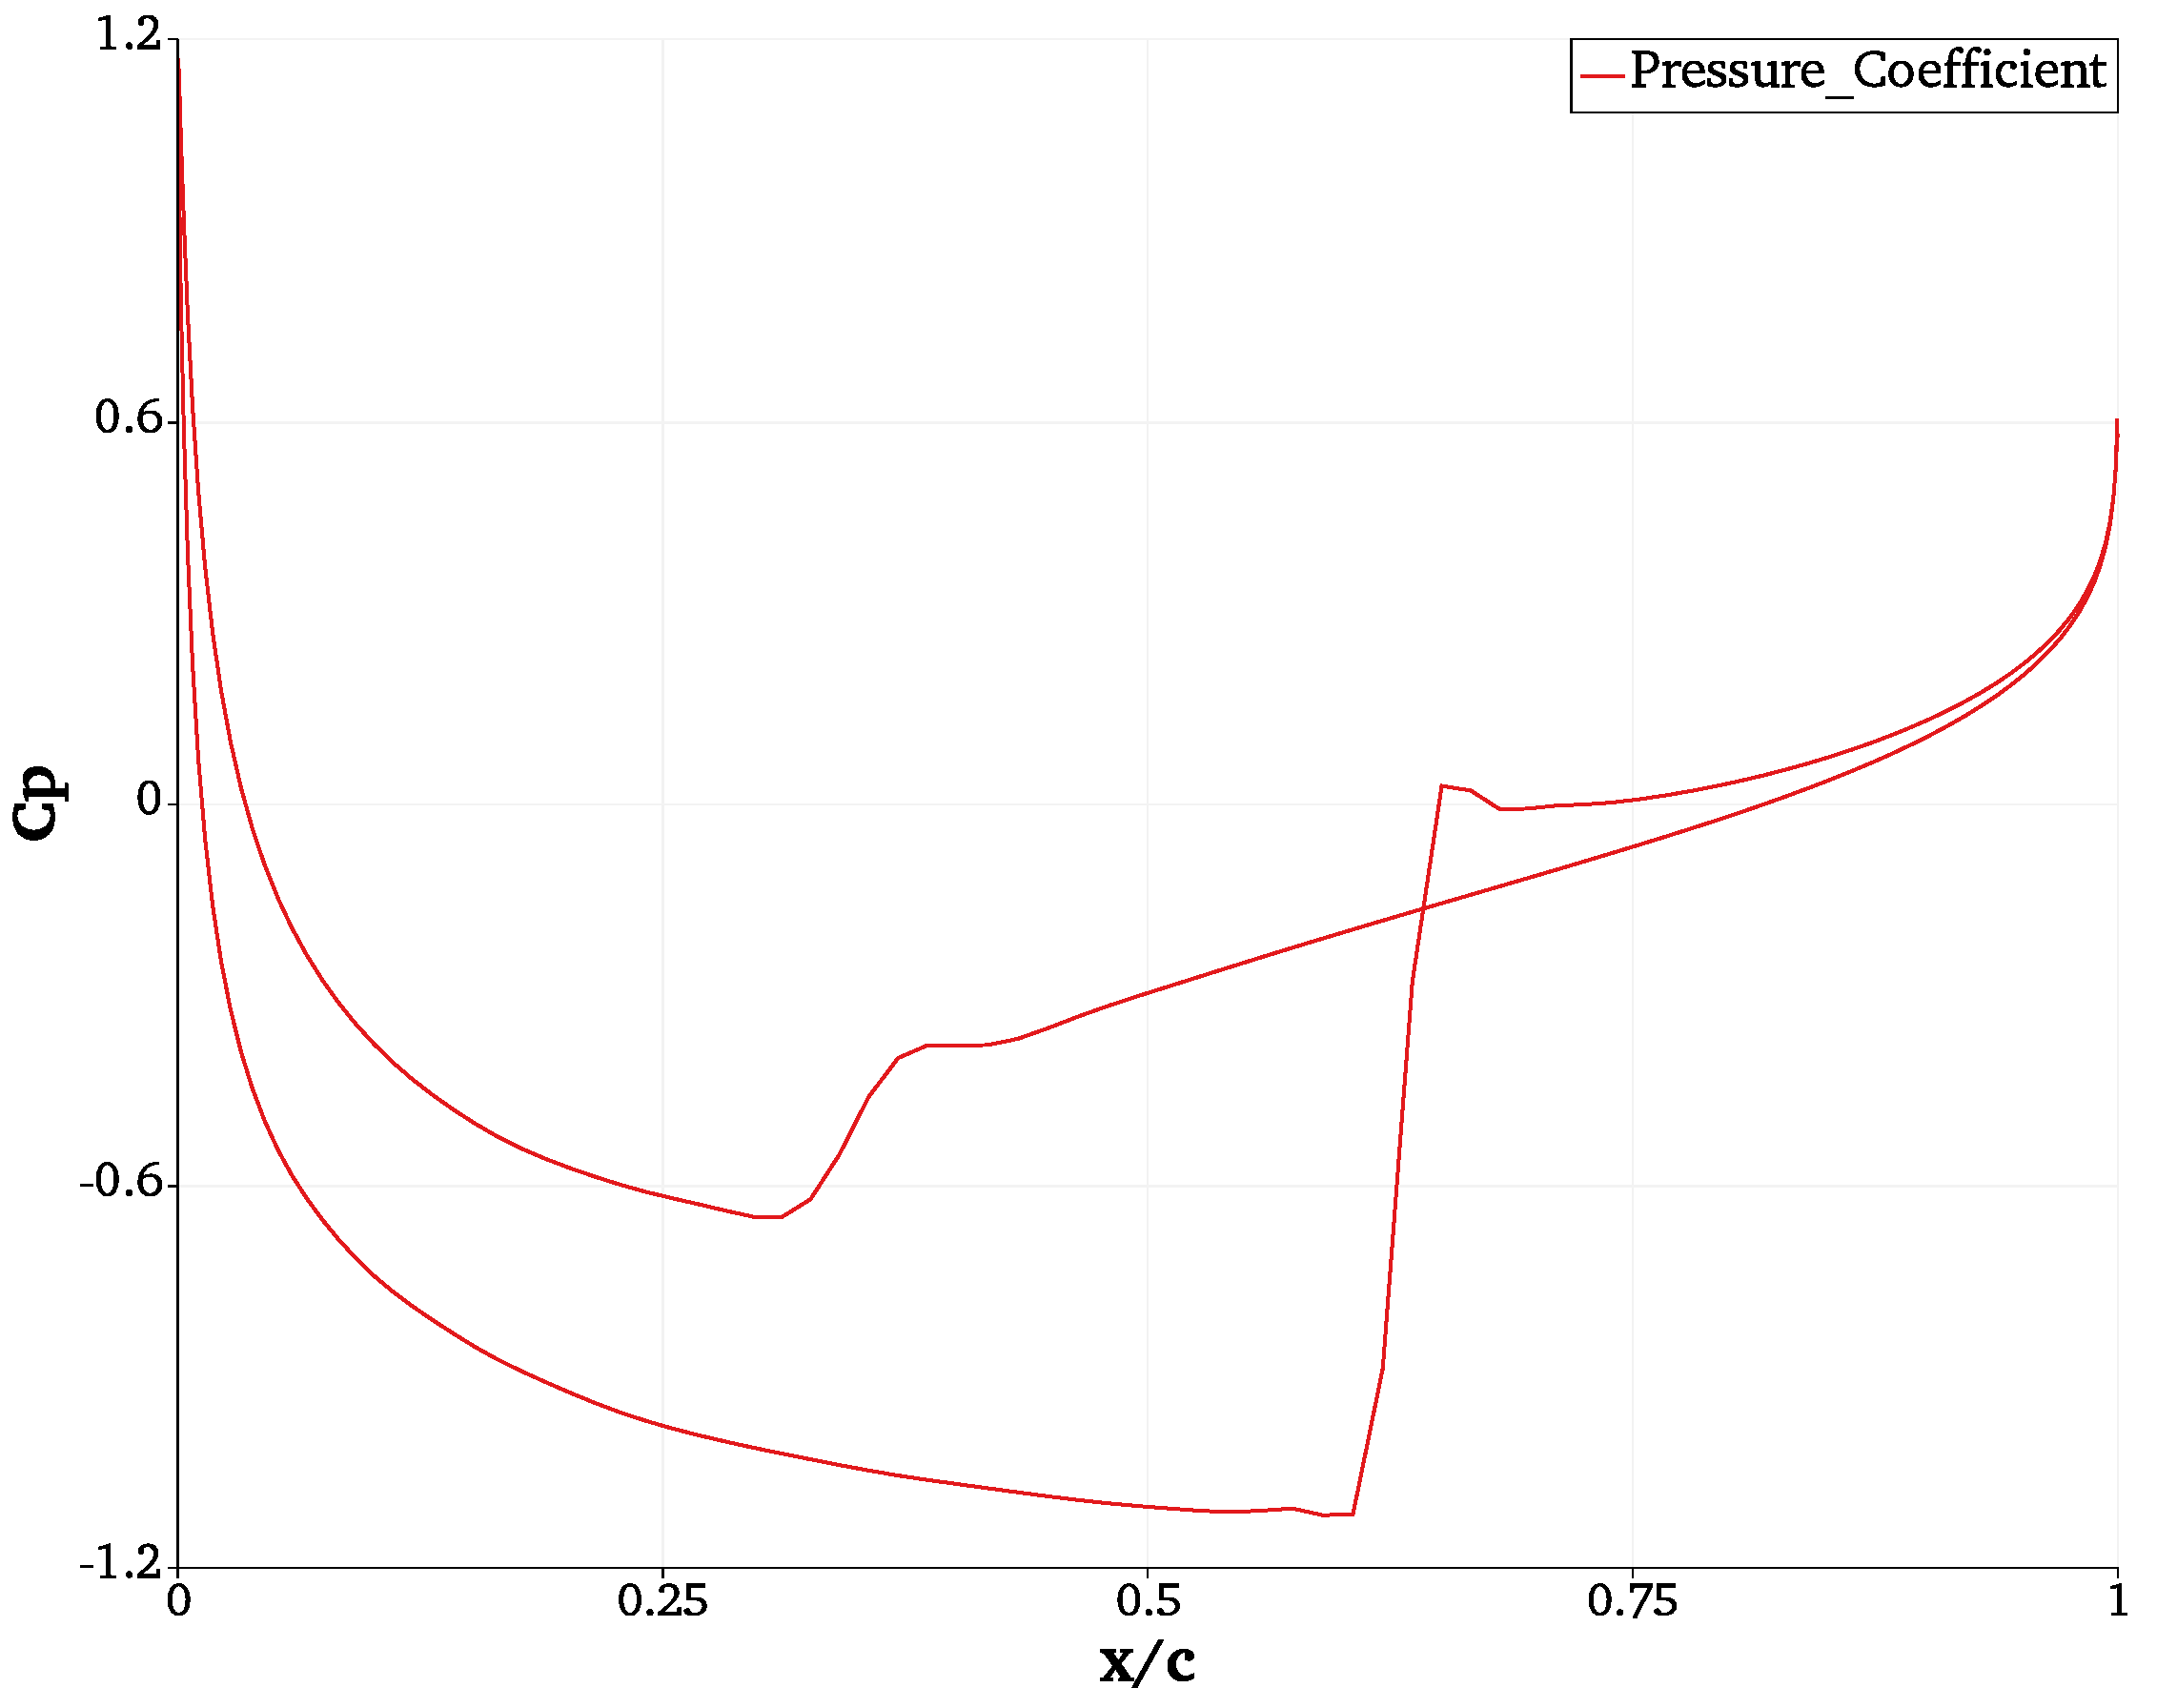
\includegraphics[width=.75\textwidth]{tut01/plot11.pdf}
    \caption{Pressure coefficient on the surface of the NACA 0012 airfoil.}
    \label{fig1:surface_pressure}
\end{figure}

By convention, $-C_p$ is typically plotted such that the pressure curve on suction side (lower pressure) is on top of the pressure curve on the pressure side (higher pressure). Therefore, we need to reverse the $y$-axis in this plot to flip it. To do this, go to \textbf{Display} in the \textbf{Properties} tab. Next, find the \textbf{Left Axis Range} section in the same tab, and then click on \textbf{Left Axis Use Custom Range} (Figure \ref{fig1:viewsetting}). Later, another section appears to select maximum/minimum ranges for the left axis of the plot. Now, switch numbers in these two text bars. This allows the $y$-axis to be reverse (flipped).
\begin{figure}[htbp]
    \centering
    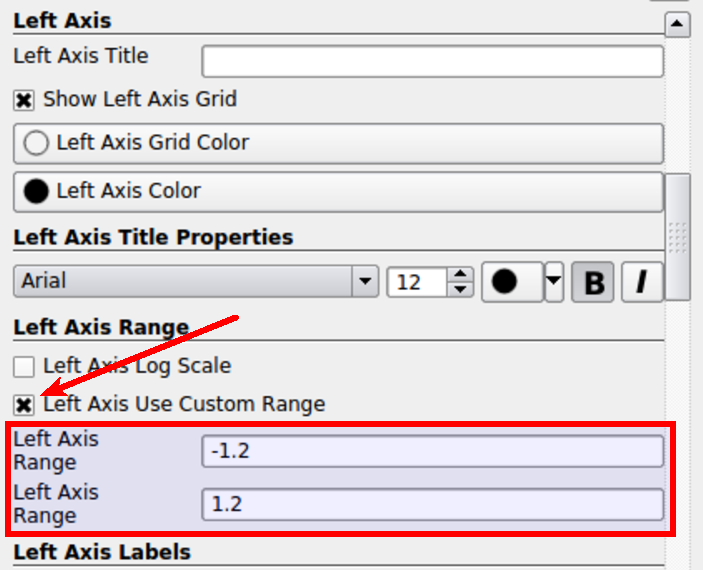
\includegraphics[width=0.5\textwidth]{tut01/leftaxis.pdf}
    \caption{Plot Settings.}
    \label{fig1:viewsetting}
\end{figure}
Additionally, there are other parameters that you may want to change in the same tab, such as the \textbf{Left Axis Title} or the \textbf{Bottom Axis Title}. Please type $C_p$ and $x/c$ in \textbf{Left Axis Title} and \textbf{Bottom Axis Title}, respectively. Furthermore, for adding markers to the plot lines, from \textbf{Display} select the \textbf{Marker Style} as \textit{Diamond} (Figure \ref{fig1:marker}). You can also change the thickness of the plot line in the same tab.
\begin{figure}[htbp]
    \centering
    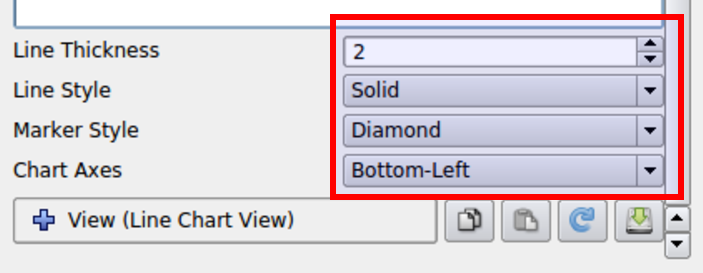
\includegraphics[width=0.4\textwidth]{tut01/addingmarker.pdf}
    \caption{How to add markers to a line plot.}
    \label{fig1:marker}
\end{figure}
The final plot you get should be similar to Figure \ref{fig1:surface_pressure2}.
\begin{figure}[htbp]
    \centering
    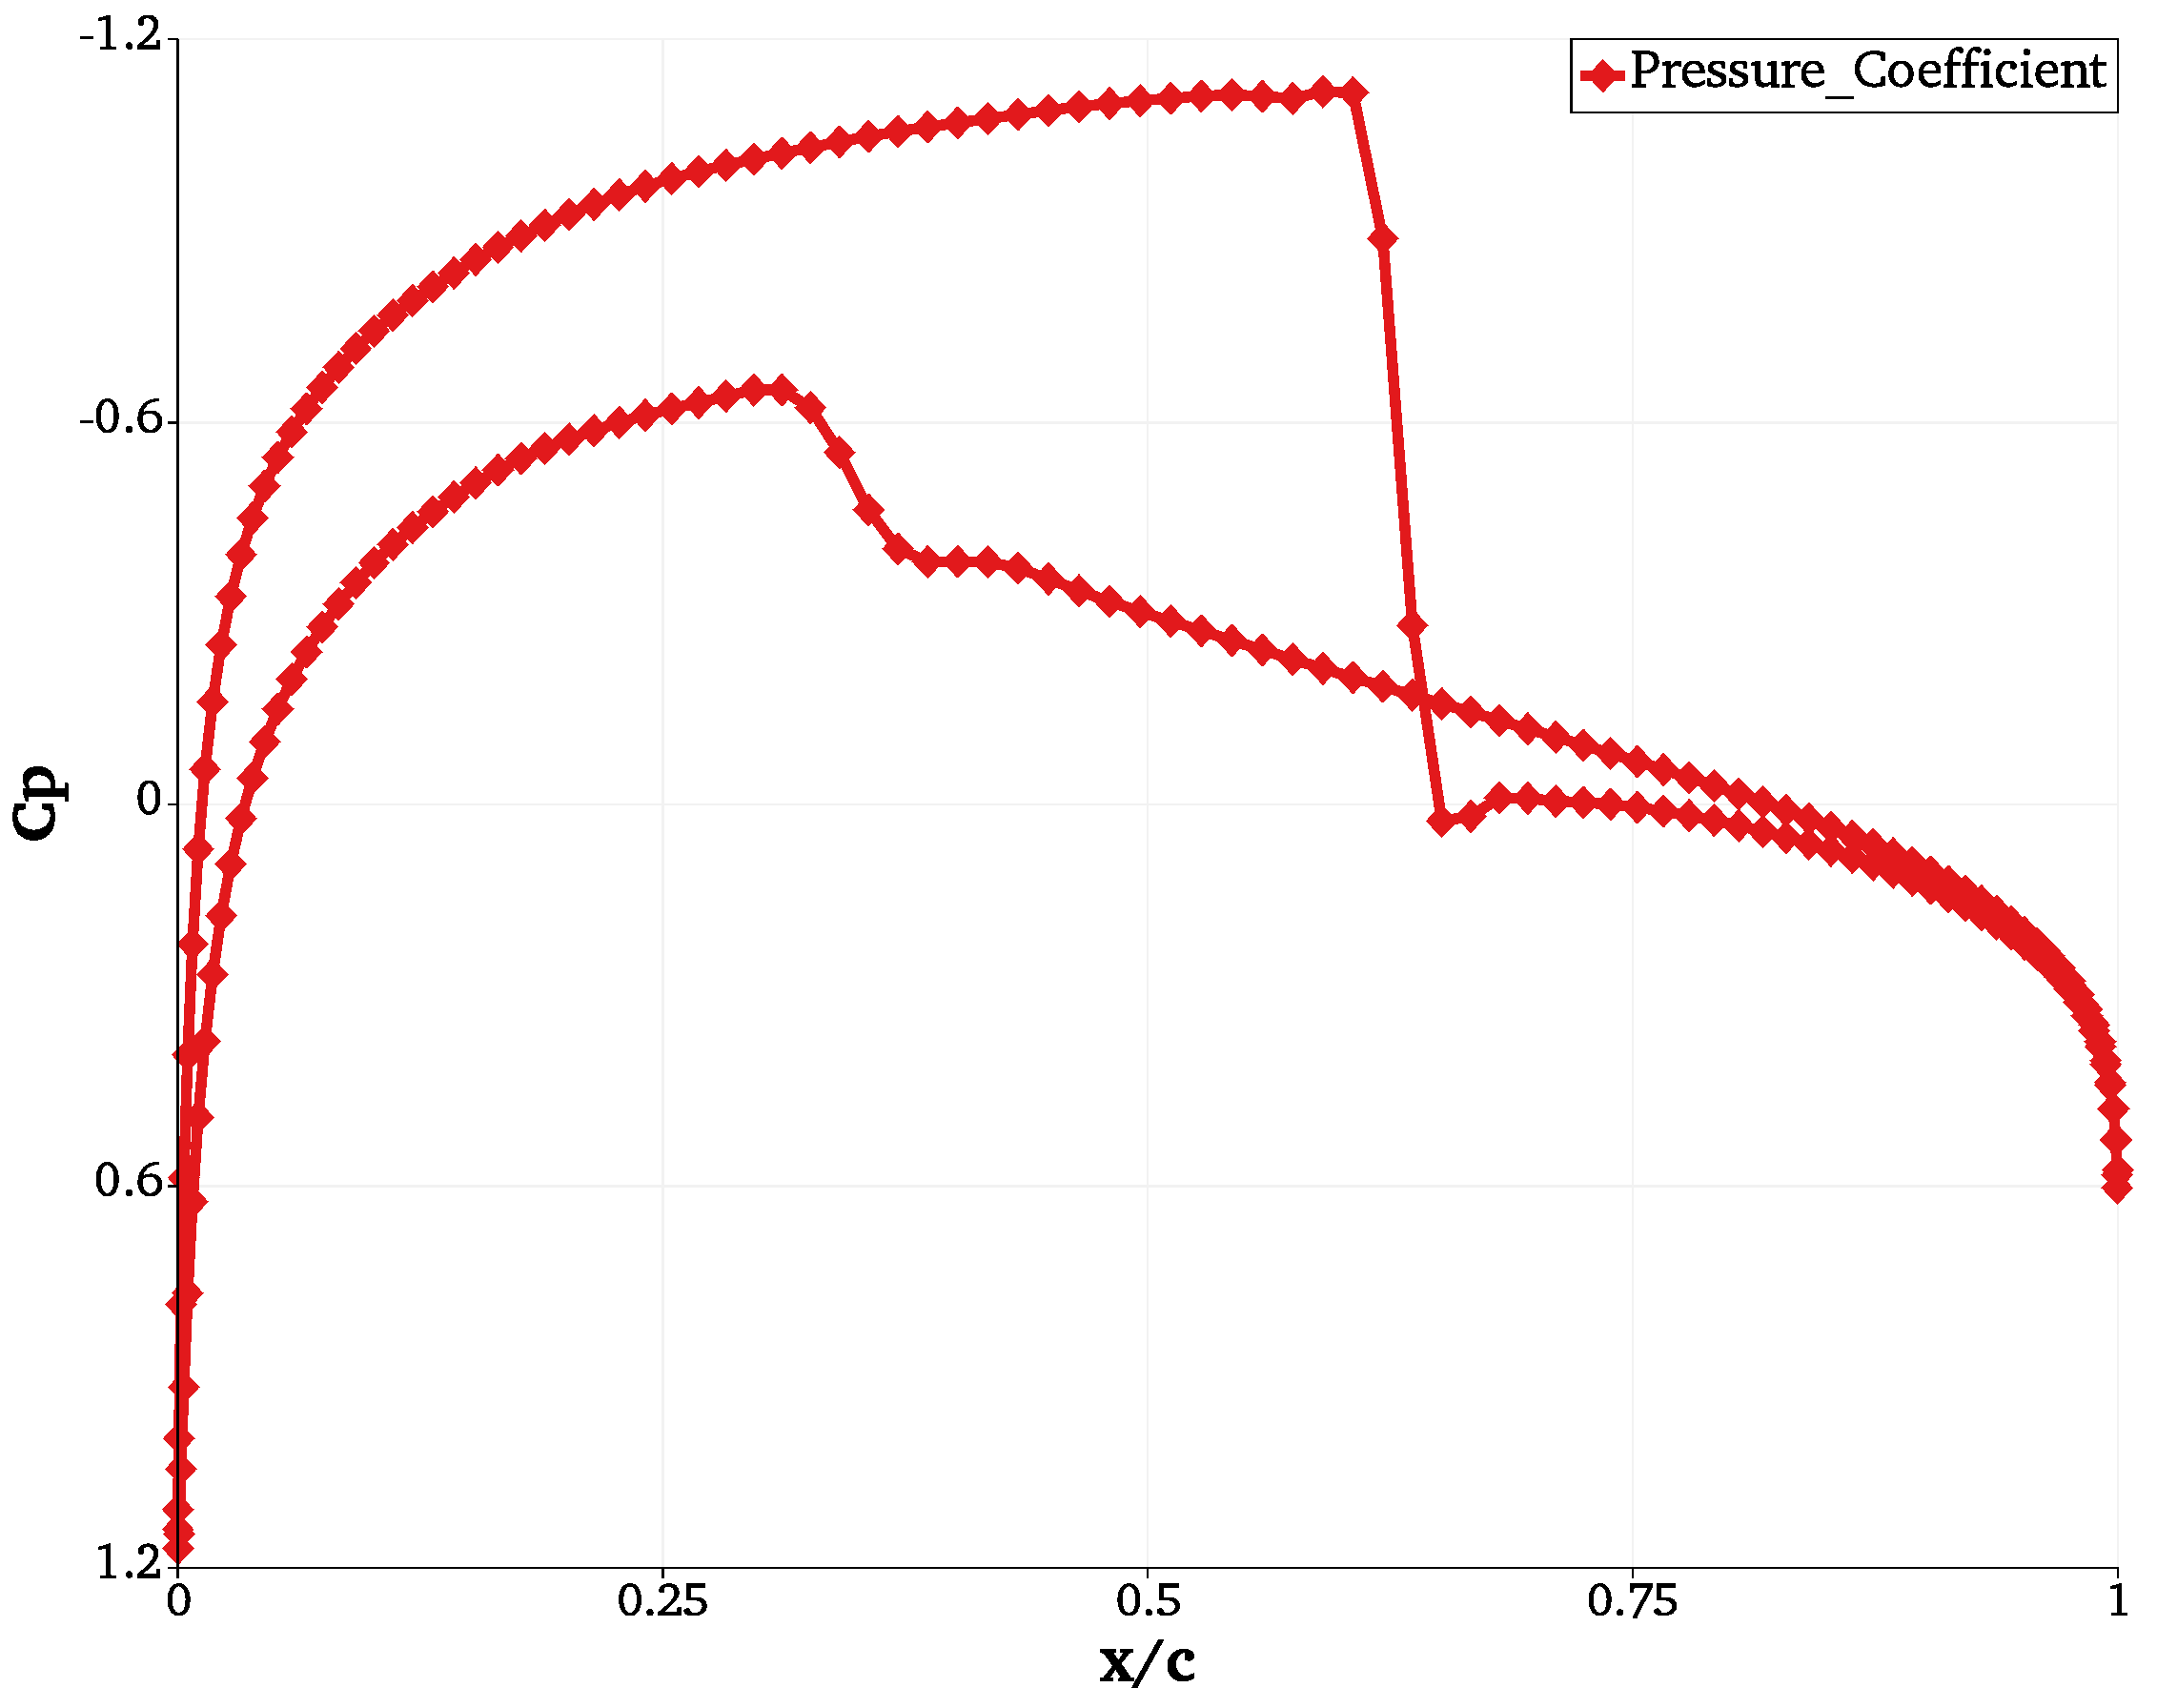
\includegraphics[width=.75\textwidth]{tut01/plot22.pdf}
    \caption{Final pressure coefficient plot on the surface of the NACA 0012 airfoil.}
    \label{fig1:surface_pressure2}
\end{figure}
%--------------------------------------------------------------
\subsection{Aerodynamic Forces}
In order to obtain the aerodynamic forces on the airfoil open \textit{force\_breakdown}.dat using a text editor. As shown in Figure \ref{fig1:forcefile1}, the flow properties are tabulated and it can be confirmed that they agree with the configuration file. 
\begin{figure}[htbp]
    \centering
    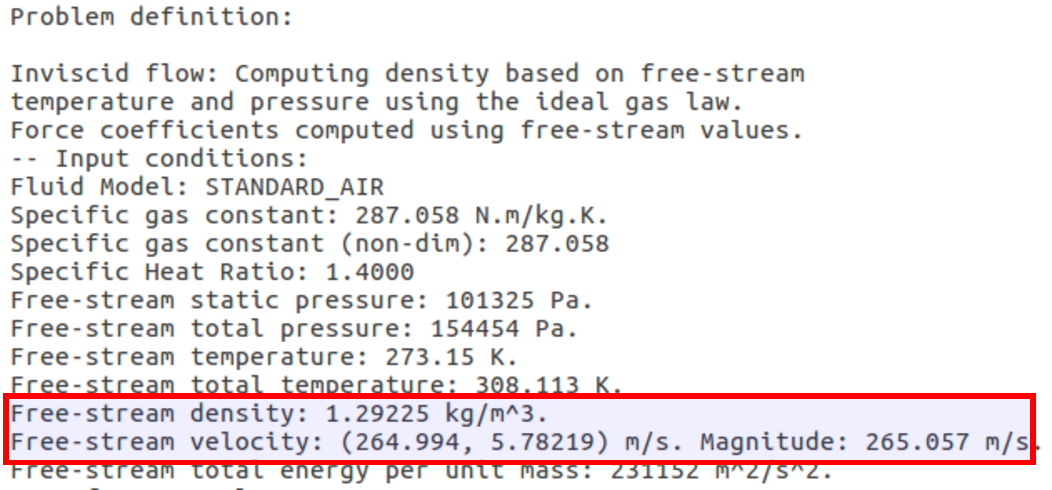
\includegraphics[width=0.9\textwidth]{tut01/forcefile1.pdf}
    \caption{Fluid and flow properties in \textit{force\_breakdown}.dat.}
    \label{fig1:forcefile1}
\end{figure}

As shown in Figure \ref{fig1:forcefile2}, the aerodynamic forces are expressed in non-dimensional form by using free-stream values for density and velocity, as well as a unit reference length in this case. The actual dimensional forces can be obtained by multiplying the flow coefficients with these non-dimensional factors calculated with the free-stream density and velocity. Note that you can find the lift coefficient ($C_L$), drag coefficient ($C_D$), lift to drag ratio ($C_L / C_D$), the moment coefficient ($C_{M,z}$), $x$-component of force coefficient ($C_{F,x}$) and $y$-component of force coefficient ($C_{F,y}$) all from the \textit{force\_breakdown}.dat file.
\begin{figure}[htbp]
    \centering
    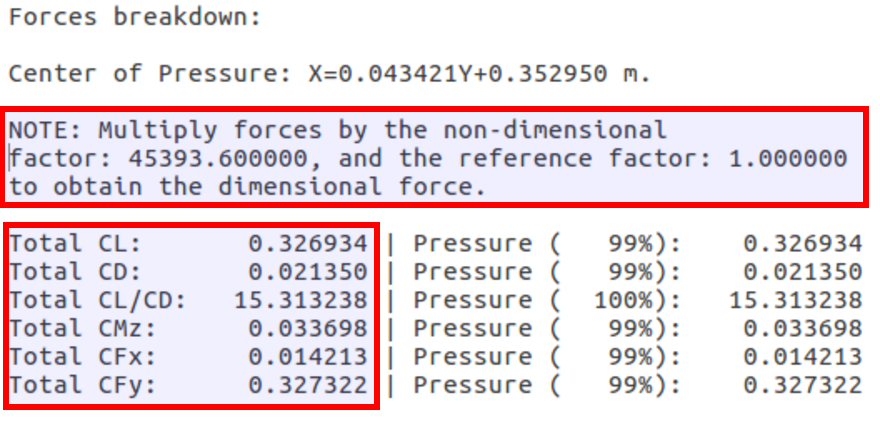
\includegraphics[width=0.8\textwidth]{tut01/forcefile2.pdf}
    \caption{Aerodynamic forces obtained from \textit{force\_breakdown}.dat.}
    \label{fig1:forcefile2}
\end{figure}
%++++++++++++++++++++++++++++++++++++++++++++++++++++++++++++++
\clearpage
\section{Questions}
1. Run the provided default NACA 0012 test case at $Ma=0.8$.
\begin{enumerate}[label=(\alph*)]
    \item Plot and comment on the mesh.
    \item Plot and comment on the pressure contours around the airfoil.
    \item Plot and comment on the pressure coefficient on the surface of the airfoil.
\end{enumerate}
2. Re-run the default NACA 0012 case but change the Mach number to $Ma=0.3$, and run several simulations using $\alpha = 0, 2, 4, 6, 8, 10, 12, 14, 16$ degrees.
\begin{enumerate}[label=(\alph*)]
    \item Plot $C_{L}$ vs $\alpha$ alongside the provided experimental data\cite{ladson1988effects} (download \href{https://gitlab.com/bvermeir/book-cfd/blob/master/tutorial/tut1_inviscid_NACA 0012/experimental_values.zip}{\underline{here}}) in the test case folder.
    \item Repeat 1.b with $Ma = 0.3$ for the $\alpha = 0, 8, 16$ degree cases.
    \item Repeat 1.c with for the $\alpha = 0, 8, 16$ degree cases, and include the provided experimental data from \cite{ladson1987pressure}.
\end{enumerate}
3. Compare your CFD results in Q.2, and discuss sources of error that could have led to any discrepancies in your results.
%--------------------------------------------------------------
%++++++++++++++++++++++++++++++++++++++++++++++++++++++++++++++
%++++++++++++++++++++++++++++++++++++++++++++++++++++++++++++++
%++++++++++++++++++++++++++++++++++++++++++++++++++++++++++++++
\chapter{Supersonic Wedge}
\label{ch:Supersonic Wedge}
%++++++++++++++++++++++++++++++++++++++++++++++++++++++++++++++
\section{Required Files}
\begin{su2note}
	Use the following links to download the same version of SU2 for Windows (\href{https://users.encs.concordia.ca/~bvermeir/book/executables/windows/SU2-v7.0.0-win64.zip}{\underline{click here}}) or Mac (\href{https://users.encs.concordia.ca/~bvermeir/book/executables/osx/SU2-v7.0.0-macos64.zip}{\underline{click here}}), and the required configuration (\href{https://gitlab.com/bvermeir/book-cfd/blob/master/tutorial/tut2_supersonic_wedge/inv_wedge_HLLC.cfg}{\underline{click here}}) and mesh files (\href{https://gitlab.com/bvermeir/book-cfd/blob/master/tutorial/tut2_supersonic_wedge/mesh_wedge_inv.su2}{\underline{click here}}).
\end{su2note}
\begin{paraviewnote}
	Use the following links to download the same version of Paraview for Windows (\href{https://users.encs.concordia.ca/~bvermeir/book/executables/windows/ParaView-5.4.0-Qt5-OpenGL2-Windows-64bit.exe}{\underline{click here}}) or Mac (\href{https://users.encs.concordia.ca/~bvermeir/book/executables/osx/ParaView-5.4.0-Qt5-OpenGL2-MPI-OSX10.8-64bit.dmg}{\underline{click here}}).
\end{paraviewnote}

\section{Problem Description}
In this tutorial we are going to demonstrate how to simulate supersonic inviscid flow past a simple 2D wedge. This wedge generates an oblique-shock wave moving outwards from its surface. Assuming the Reynolds number is high, and that the fluid is an ideal gas, we will be using the Euler equations. The domain is approximated using a structured mesh with 3,750 nodes. The domain consists of a flat upper wall, and a lower wall with an inclined a wedge starting at $x/L=1/3$, where $L$ is the length of duct. The wedge angle is taken to be 10 degrees, and the inlet flow paramaters are:
\begin{itemize}
    \item Pressure = 101,325 Pa
    \item Temperature = 273.15 K
    \item Mach number = 2.0
    \item Wedge angle = 10 degrees
\end{itemize}
This tutorial has two parts: Flow Solution and Post-processing. In the first part, we will explain how to manage the prerequisite files and settings, and how to run the CFD simulation using SU2. In the second part we explain how to use Paraview to visualize the data obtained from SU2.
%++++++++++++++++++++++++++++++++++++++++++++++++++++++++++++++
\section{Flow solution}
To run this simulation SU2 needs two files: a configuration file (.cfg) and a mesh file (.su2). Links to the required files and executables are provided at the start of this tutorial. The files include:
\begin{enumerate}
    \item inv\_wedge\_HLLC.cfg which is a configuration file.
    \item mesh\_wedge\_inv.su2 which is a a mesh file.
\end{enumerate}
The next step is to copy these two files into the same directory as the SU2 executable. Then, to run the simulation open a terminal window and enter the following commands:
\begin{table}[htbp]
    \centering
    \begin{tabular}{|l|l|}
    \hline
    Windows     & \begin{tabular}{c} \$ cd "where you saved the package" \\ \$ SU2\_CFD.exe inv\_wedge\_HLLC.cfg \end{tabular}
    \\
    \hline
    Mac     & \begin{tabular}{c} \$ cd "where you saved the package" \\ \$ SU2\_CFD.exe inv\_wedge\_HLLC.cfg \end{tabular}
    \\
    \hline
    \end{tabular}
\end{table}

The SU2 solver will commence solving the problem and will print out the residuals at every iteration, until the specified convergence criteria is achieved. After the calculations are complete the following output files should have been generated within in the SU2 folder:
\begin{itemize}
    \item \textit{flow}.vtk: The flow solution on the entire domain.
    \item \textit{force\_breakdown}.dat: Forces and moment on the airfoil.
    \item \textit{history}.vtk: Convergence history.
    \item \textit{restart\_flow}.dat: Restart file.
    \item \textit{surface\_flow}.vtk: The flow solution on the airfoil surface.
    \item \textit{surface\_flow}.csv: A comma separated value file of the flow solution on the airfoil.
\end{itemize}
Please keep in mind that every time you run SU2, the output data will be overwritten. Hence, before launching a new simulation you should backup your files in another directory.
%++++++++++++++++++++++++++++++++++++++++++++++++++++++++++++++
\section{Post-Processing}
In this section, we explain how to use Paraview to visualize the solution generated by SU2. First of all, install paraview (if not already done) using the links at the start of this tutorial. Once that is complete, perform the following steps to visualize the results:
%--------------------------------------------------------------
\subsection{Load the Solution File:}
Launch Paraview. Go to \textbf{File} $\rightarrow$ \textbf{Open}, and then select the \textit{flow}.vtk file. On the left side of the Paraview window you will see the file appears in the \textbf{Pipeline Browser} under \textbf{builtin}. Now press the \textbf{Apply} button in the \textbf{Properties} tab, right under the \textbf{Pipeline Browser} heading. After taking these steps, your file is loaded by Paraview and is ready to be visualized (Figure \ref{fig2:load}).
\begin{figure}[htbp]
    \centering
    \includegraphics[width=0.4\textwidth]{tut02/loadvtkfile.pdf}
    \caption{Loading the .vtk file into the \textbf{Pipeline Browser}.}
    \label{fig2:load}
\end{figure}
%--------------------------------------------------------------
\subsection{Visualize the Mesh}
As shown in Figure \ref{fig2:wireframe}, in order to view the mesh select \textit{Solid Color} with \textit{Wireframe} in the toolbar. Then, you can zoom in to see the mesh for the computational domain, as shown in Figure \ref{fig2:mesh}. As you can see, the mesh in the duct is structured, and the wedge abruptly changes the direction of mesh on the bottom surface. Additionally, the grids are approximately uniform throughout the domain.
\begin{figure}[htbp]
    \centering
    \includegraphics[width=0.6\textwidth]{tut02/wireframe.pdf}
    \caption{How to display the mesh.}
    \label{fig2:wireframe}
\end{figure}
\begin{figure}[htbp]
    \centering
    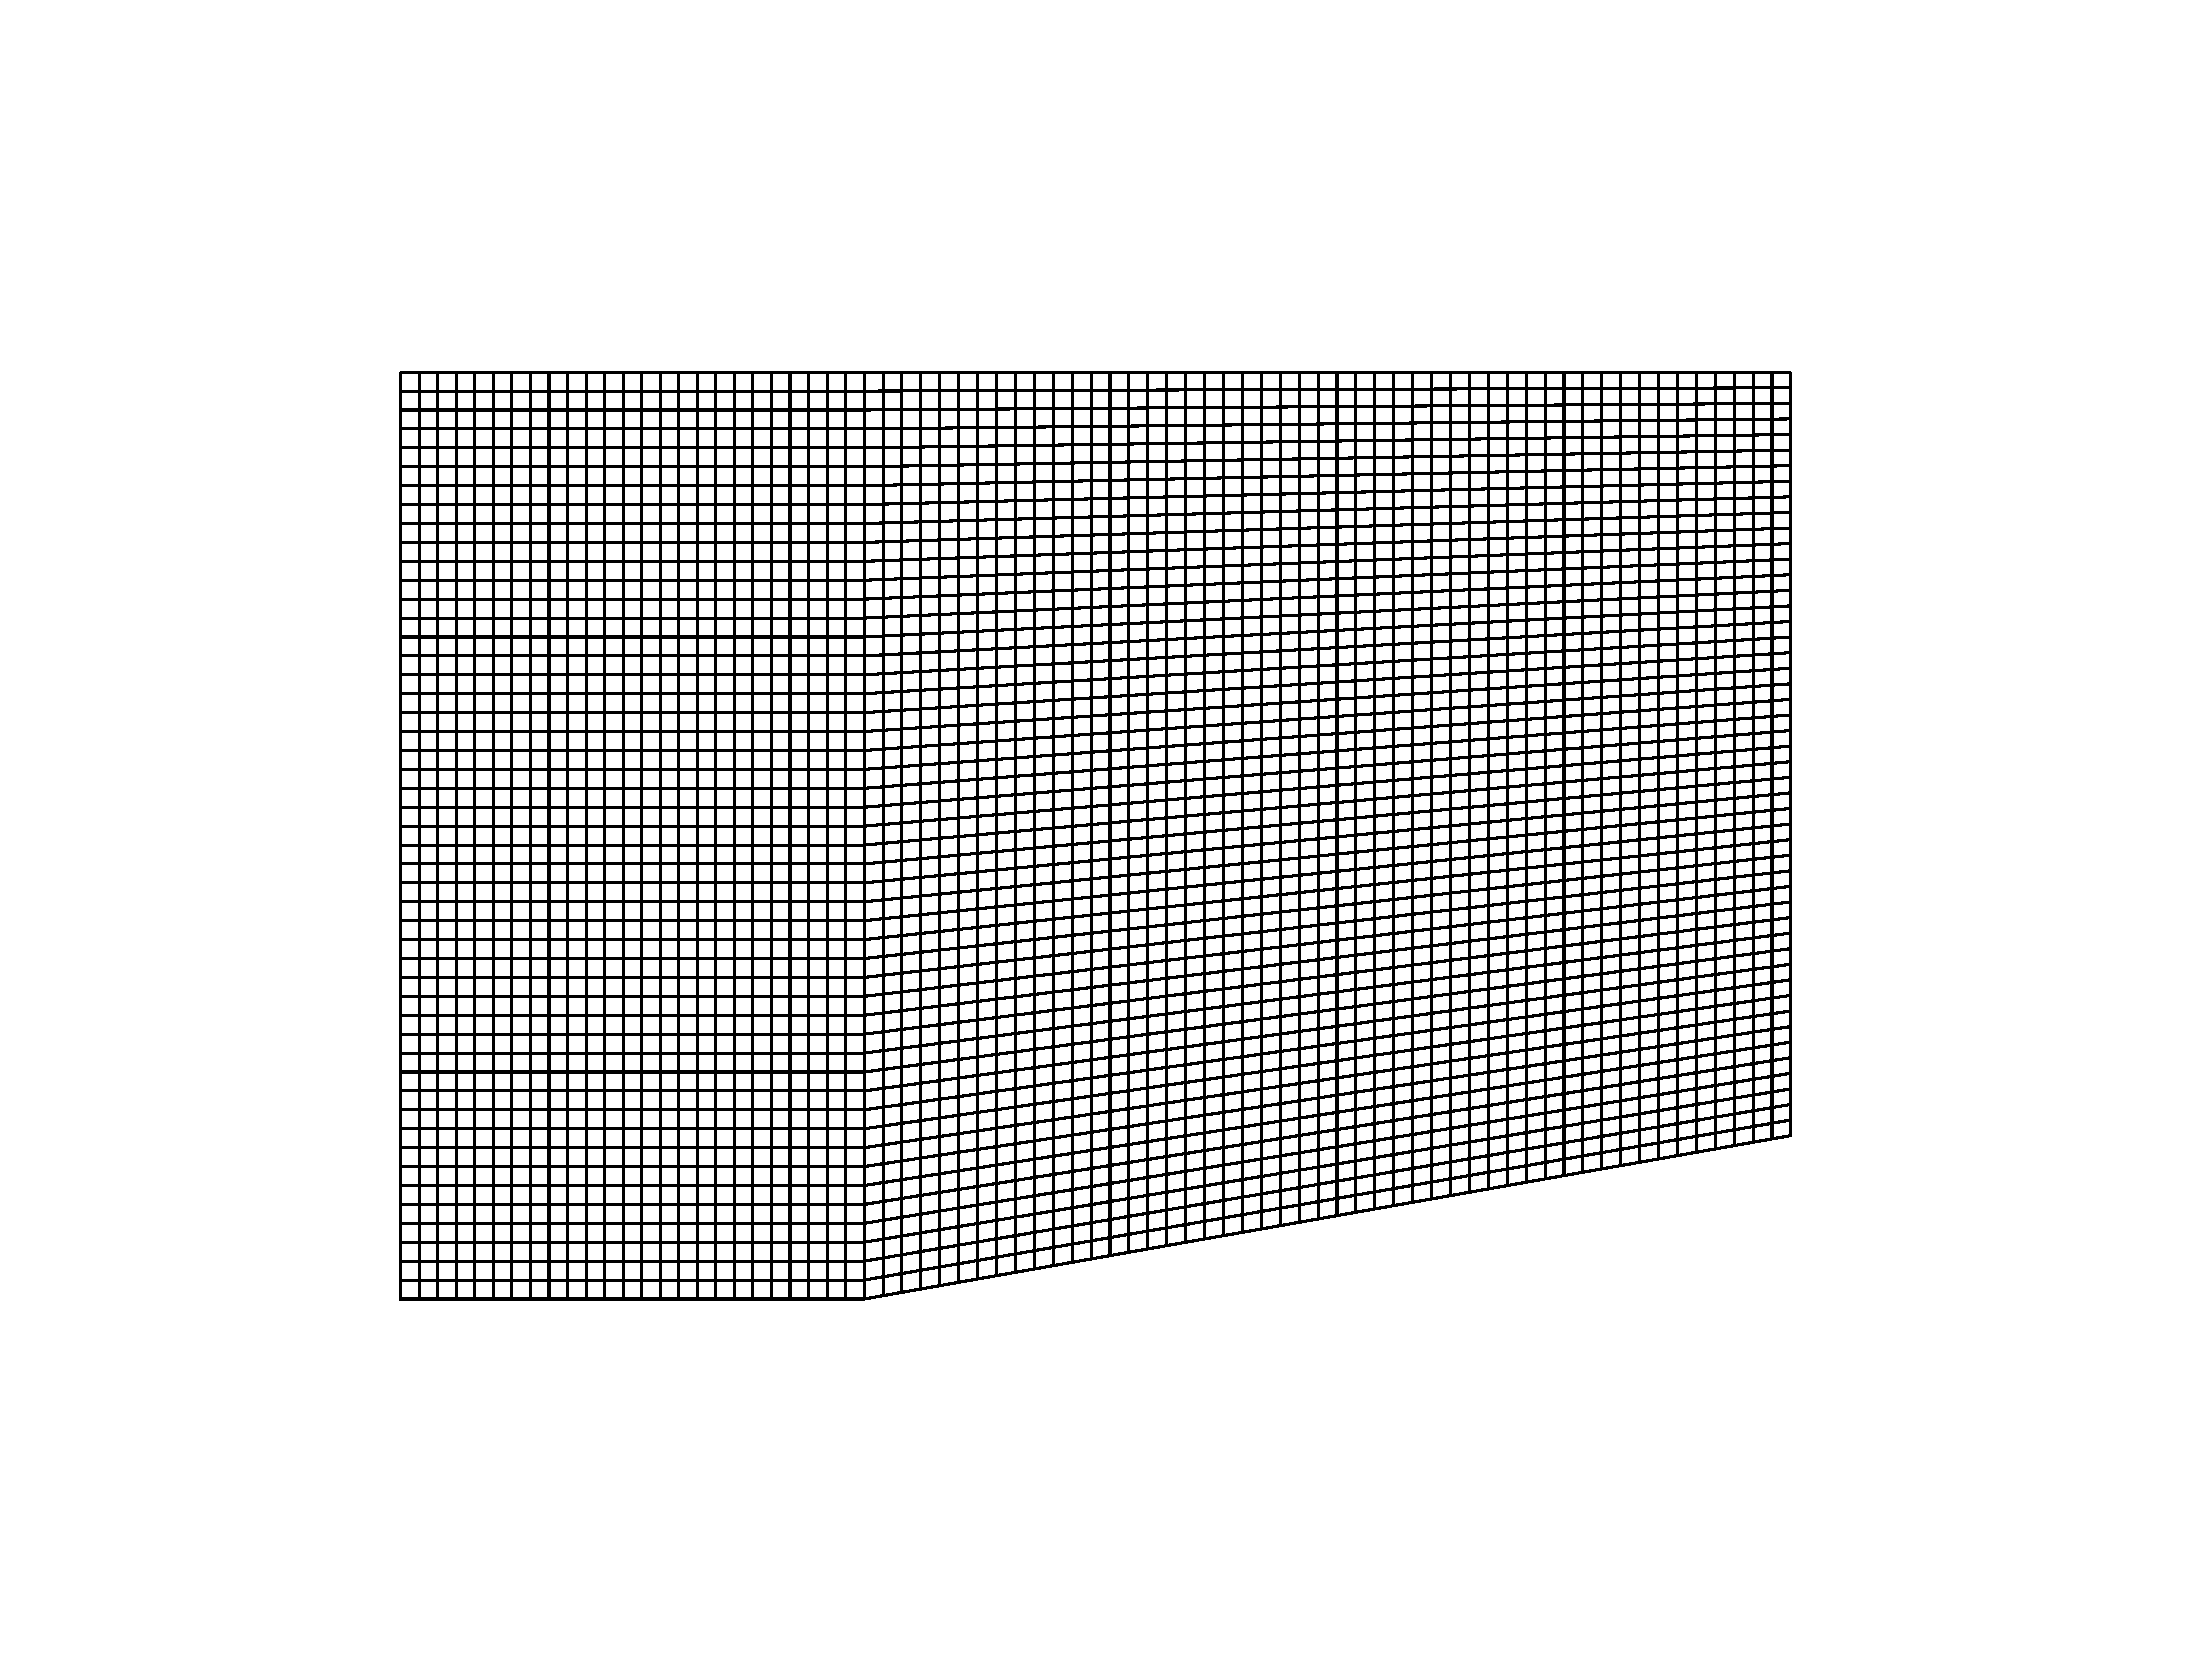
\includegraphics[width=.75\textwidth]{tut02/mesh.pdf}
    \caption{The structured mesh for the supersonic wedge.}
    \label{fig2:mesh}
\end{figure}
%--------------------------------------------------------------
\subsection{Visualize Pressure and Mach Contours}
To display pressure contours click on \textit{flow}.vtk in the \textbf{Pipeline Browser}, and then click on the \textbf{Display} form in the \textbf{Properties} tab. Under the \textbf{Coloring} section select \textit{Pressure} from the drop-down menu (Figure \ref{fig2:pressure contours setting}). Additionally, to change the color settings used for pressure you can click on the \textbf{Edit} option under the \textbf{Coloring} section.
\begin{figure}[htbp]
    \centering
    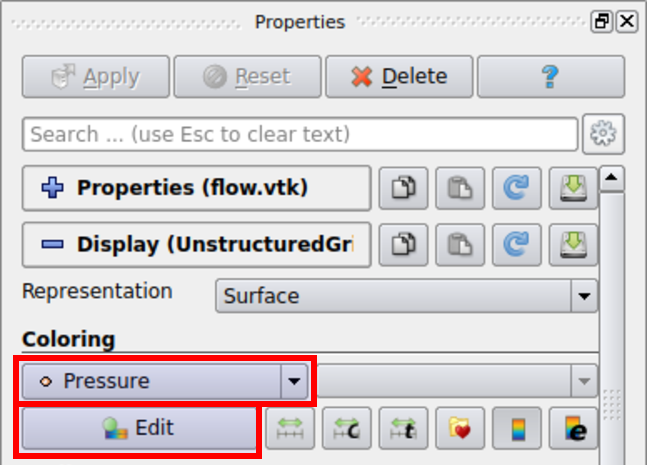
\includegraphics[width=0.4\textwidth]{tut02/pressurecont.pdf}
    \caption{Settings for displaying pressure contours.}
    \label{fig2:pressure contours setting}
\end{figure}
Another display window will appear on the right-hand side of the menu entitled \textbf{Mapping Data}, similar to Figure \ref{fig2:color_range}.
\begin{figure}[htbp]
    \centering
    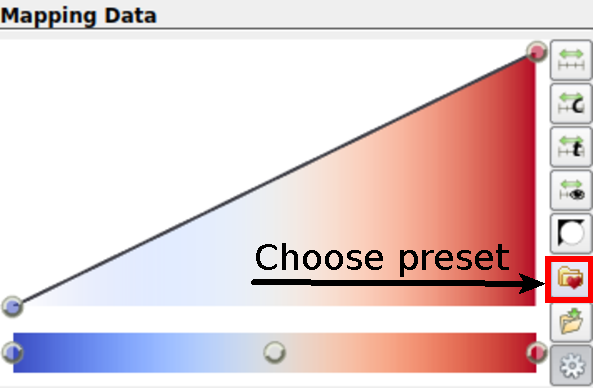
\includegraphics[width=0.4\textwidth]{tut02/colorrange.pdf}
    \caption{Changing the color range used for pressure contours.}
    \label{fig2:color_range}
\end{figure}
Now you can change contour colors by choosing \textbf{Choose preset}. Here, we select the \textit{Cold and Hot} color scale, to be able to show clearly the sharp changes in pressure values around the shock (Figure \ref{fig2:color_range_item}). Then, click \textbf{Apply}.
\begin{figure}[htbp]
    \centering
    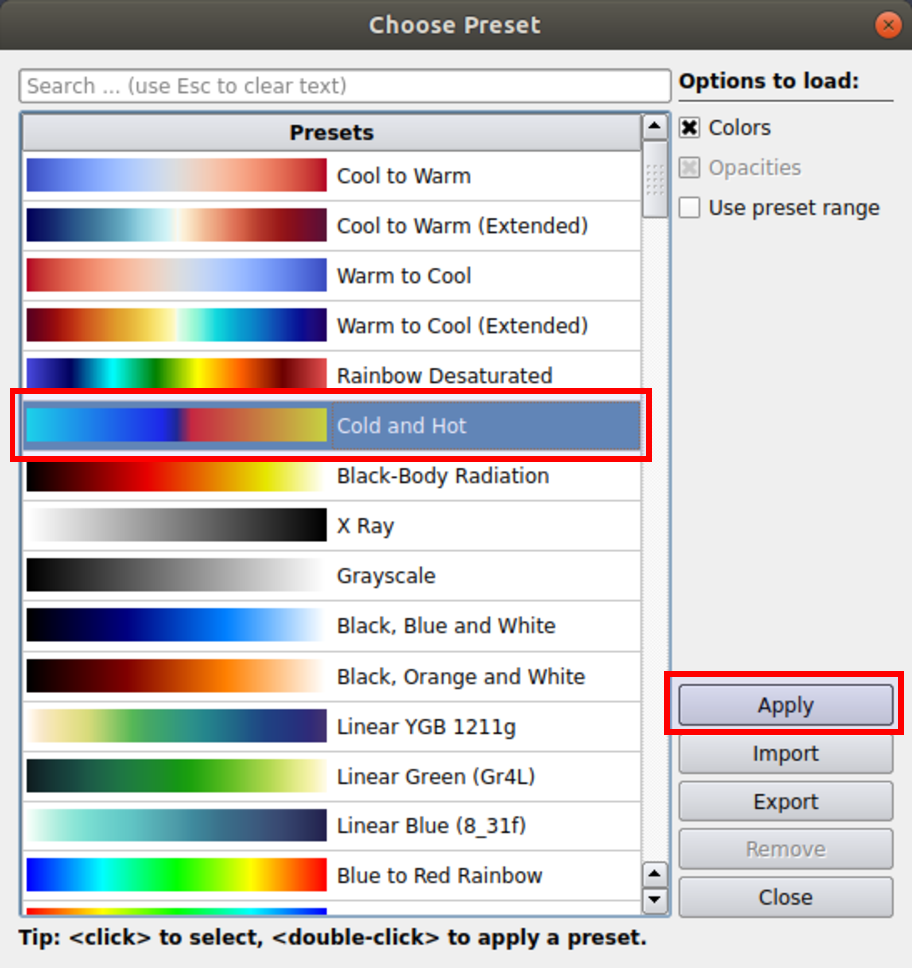
\includegraphics[width=0.5\textwidth]{tut02/changecontourcolors.pdf}
    \caption{Different color ranges used to display contours.}
    \label{fig2:color_range_item}
\end{figure}
To add axes to the plots look under the \textbf{Miscellaneous} form of the \textbf{Display} field (Figure \ref{fig2:add axis}) and select the check box beside \textbf{Data Axes Grid}. Then go to \textbf{Edit} and change these options based on your preferences (Figure \ref{fig2:axis setting}).
\begin{figure}[htbp]
    \centering
    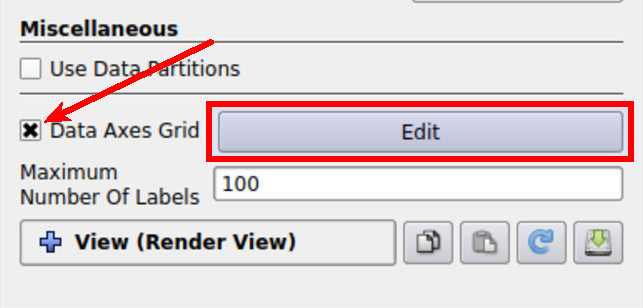
\includegraphics[width=0.4\textwidth]{tut02/addaxis.pdf}
    \caption{How to add axes to the plots.}
    \label{fig2:add axis}
\end{figure}
\begin{figure}[htbp]
    \centering
    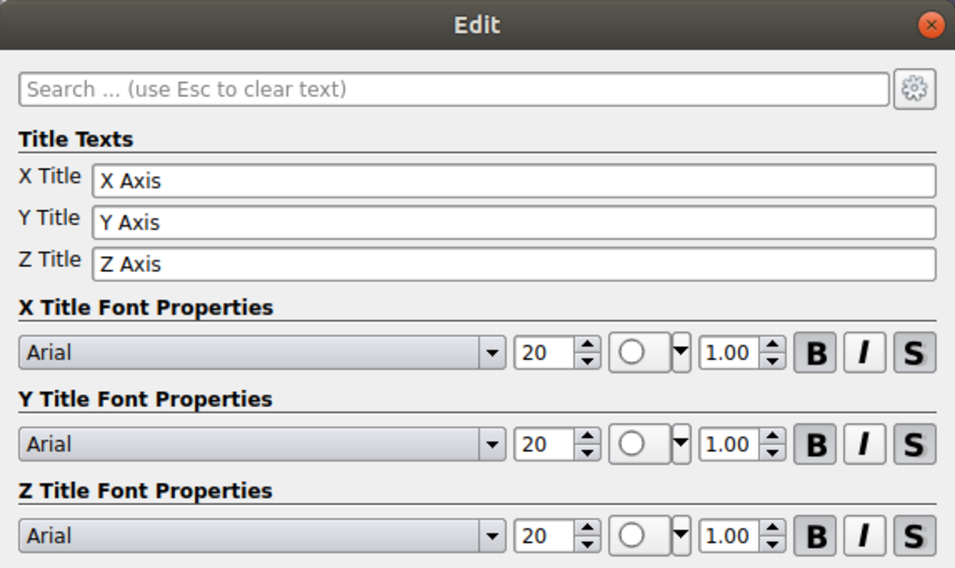
\includegraphics[width=0.6\textwidth]{tut02/axissettings.pdf}
    \caption{Settings for the axis style.}
    \label{fig2:axis setting}
\end{figure}
Finally, the pressure contour you get should be similar to Figure \ref{fig2:plot pressure cont1}.
\begin{figure}[htbp]
    \centering
    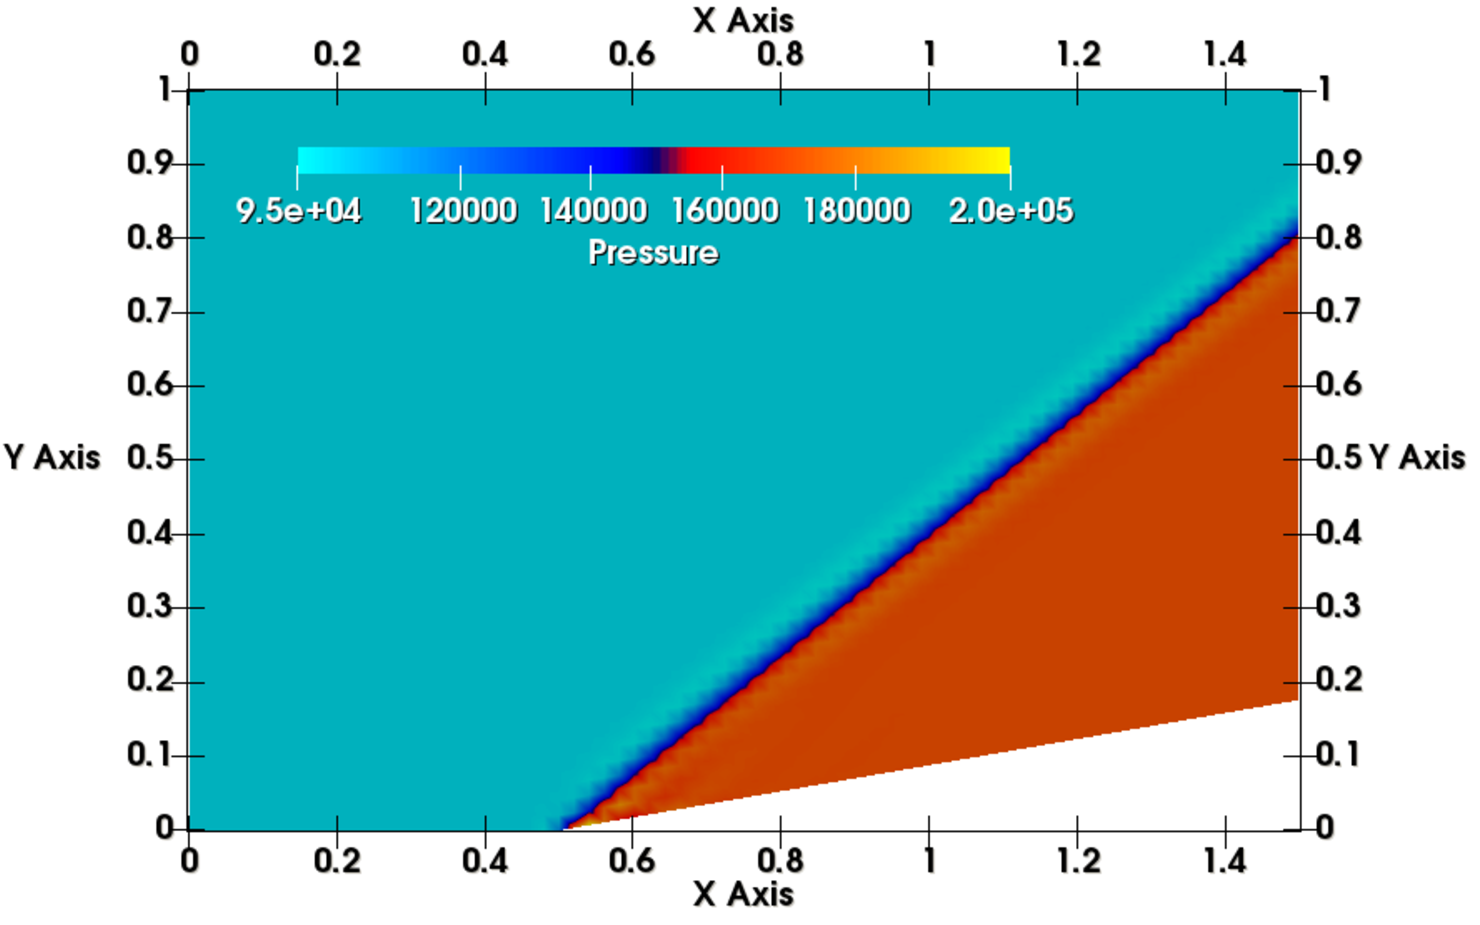
\includegraphics[width=0.85\textwidth]{tut02/plot1pressurecont.pdf}
    \caption{Pressure contours for the supersonic wedge case.}
    \label{fig2:plot pressure cont1}
\end{figure}
%----------------------------------------------------------

The pressure gradient along the shock wave is difficult to visualize directly from these contours. To help, we can add contour lines to clearly delineate the different regions. To add contour lines, click on the \textit{flow}.vtk file in the \textbf{Pipeline Browser}, and then click on the \textbf{Contour} icon (Figure \ref{fig2:contour_icon}) in the toolbar.
\begin{figure}[htbp]
    \centering
    \includegraphics[width=0.5\textwidth]{tut02/contourlineicon.pdf}
    \caption{\textbf{Contour} icon in the toolbar.}
    \label{fig2:contour_icon}
\end{figure}
Now a new \textit{Contour1} item appears under the \textit{flow}.vtk file in the \textbf{Pipeline Browser} (Figure \ref{fig2:contour1}). Click on \textbf{Apply} to proceed to the next step.
\begin{figure}[htbp]
    \centering
    \includegraphics[width=0.4\textwidth]{tut02/contour1.pdf}
    \caption{Adding \textit{Contour1} to the \textbf{Pipeline Browser}.}
    \label{fig2:contour1}
\end{figure}
With regard to Figure \ref{fig2:contourby a}, go to the \textbf{Properties} tab and select \textit{Pressure} from the \textbf{Contour By} drop-down menu. Next, click on the \textbf{Add Range} icon to customize the range to be used for the pressure contours. In Figure \ref{fig2:contourby b}, you will see the max/min range of contour lines (i.e. \textbf{From}/\textbf{To}), as well as number of lines you would like to have in your contour plot (i.e. \textbf{Steps}). Next, set \textbf{Steps} to 20, and click \textbf{OK}. By doing this the pressure contour range is equally divided into 20 lines. At the end, click on \textbf{Apply} to see contour lines in the display window.
\begin{figure}[htbp]
    \centering
     \begin{subfigure}[b]{.4\textwidth}
         \centering
         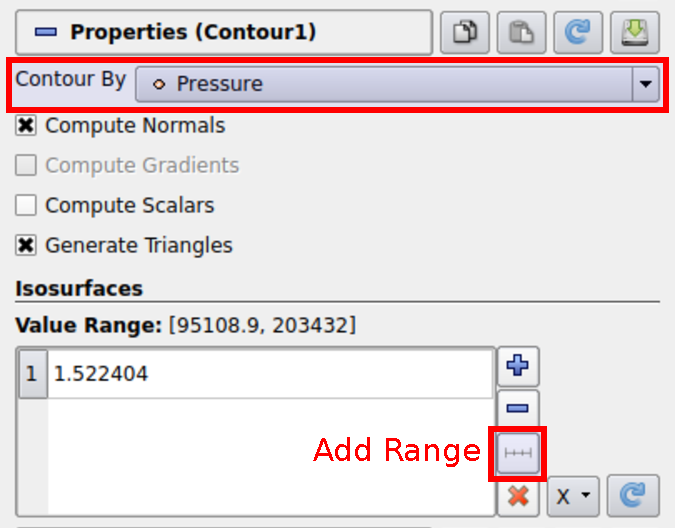
\includegraphics[width=1.0\textwidth]{tut02/contourby.pdf}
         \caption{Define a new range}
         \label{fig2:contourby a}
     \end{subfigure}
     \hfill
     \begin{subfigure}[b]{.4\textwidth}
         \centering
         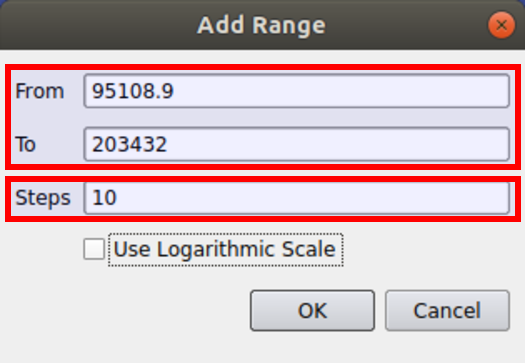
\includegraphics[width=1.0\textwidth]{tut02/addrange.pdf}
         \caption{Add range}
         \label{fig2:contourby b}
     \end{subfigure}     
    \caption{How to define a new range for the contour lines.}
    \label{fig2:contourby}
\end{figure}
Next, as shown in Figure \ref{fig2:colorby2}, click on \textbf{Display} under the \textbf{Properties} tab. In the \textbf{Coloring} section select \textbf{Solid Color} from the drop-down menu and choose white from \textbf{Edit}.
\begin{figure}[htbp]
    \centering
    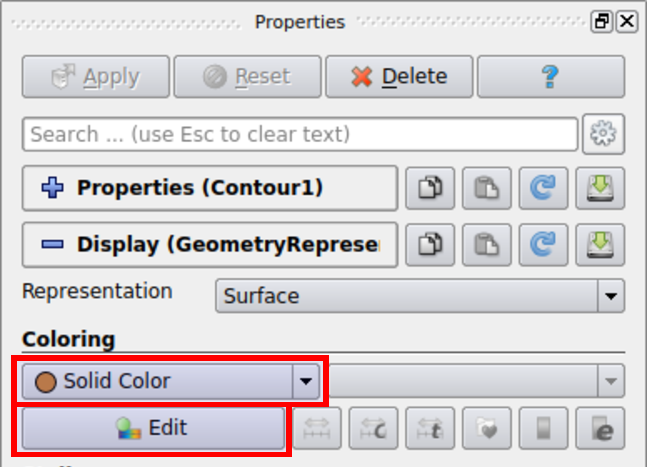
\includegraphics[width=0.4\textwidth]{tut02/contourline.pdf}
    \caption{Changing contour line colors in the \textbf{Coloring} section.}
    \label{fig2:colorby2}
\end{figure}
The pressure contour lines should now be similar to those in Figure \ref{fig2:pressure_contour_lines}.
\begin{figure}[htbp]
    \centering
    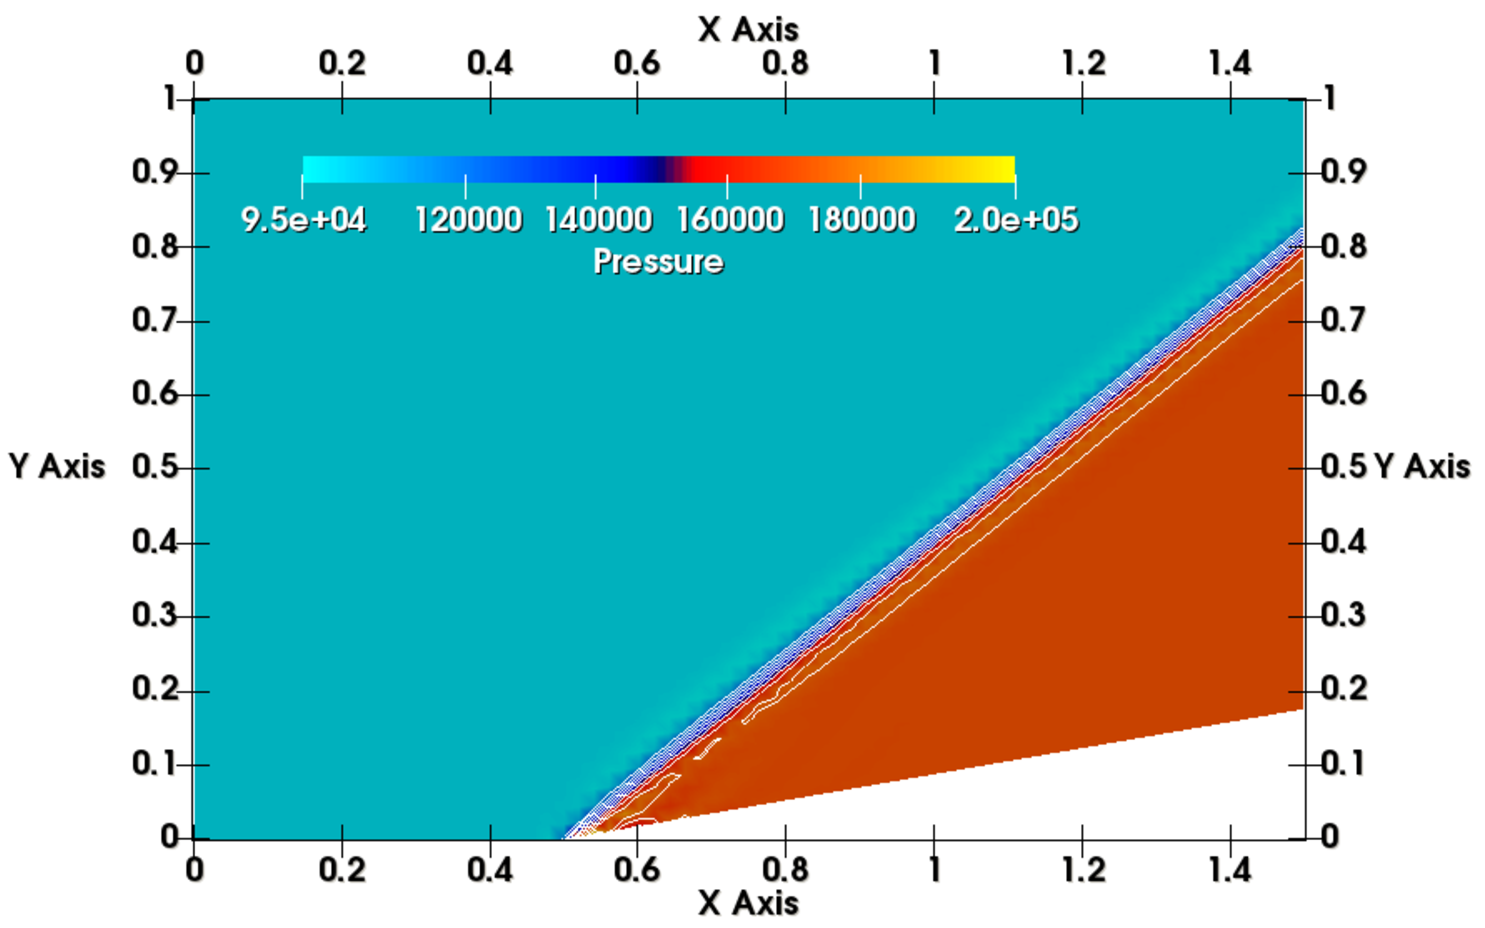
\includegraphics[width=.85\textwidth]{tut02/plot2pressurecont.pdf}
    \caption{Pressure contours superimposed by contour lines for the supersonic wedge case.}
    \label{fig2:pressure_contour_lines}
\end{figure}
You can zoom-in to the region at the bottom of the wedge to see the pressure gradient along the oblique
shock, as shown in Figure \ref{fig2:pressure_contour_lines_zoom}.
\begin{figure}[htbp]
    \centering
    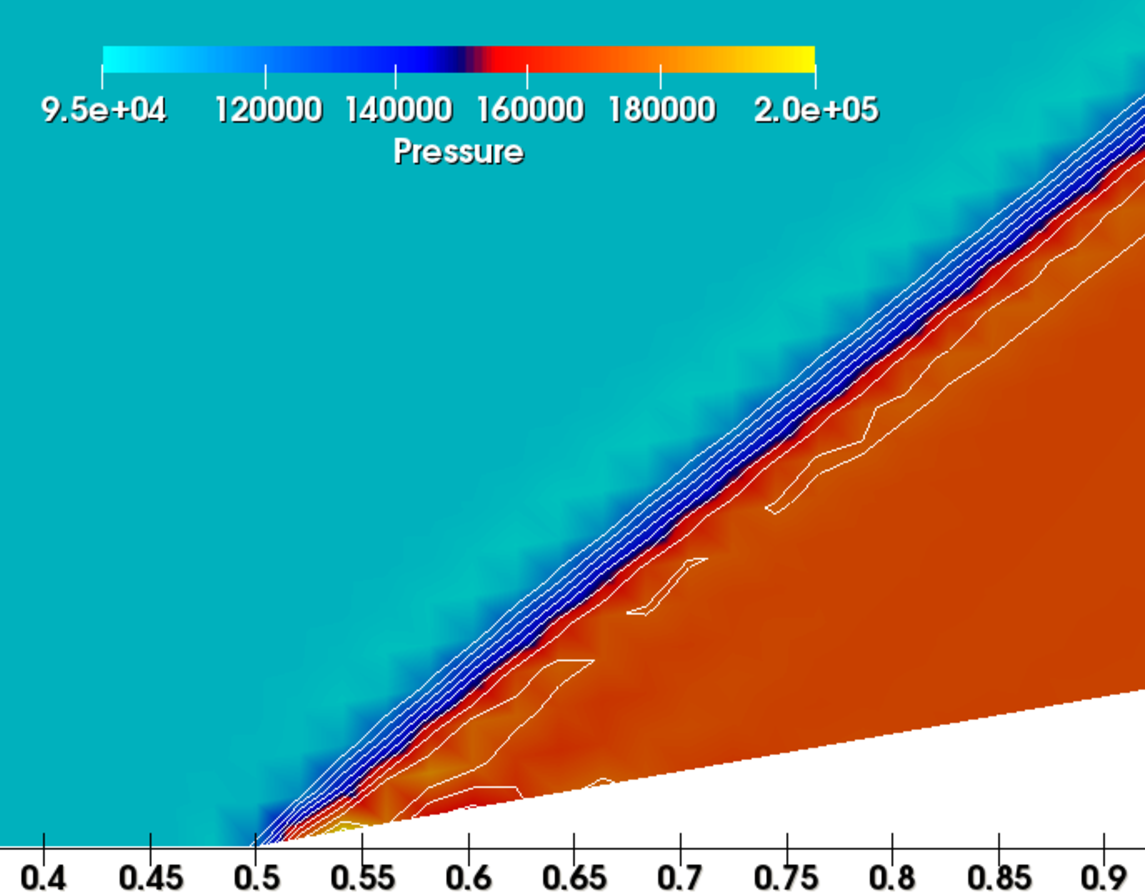
\includegraphics[width=.65\textwidth]{tut02/plot3pressurecont.pdf}
    \caption{Magnified pressure contour superimposed with contour lines for the supersonic wedge case.}
    \label{fig2:pressure_contour_lines_zoom}
\end{figure}

To display the Mach number contours click on \textit{flow}.vtk in the \textbf{Pipeline Browser}. Similar to Figure \ref{fig2:pressure contours setting}, under the \textbf{Coloring} section select \textit{Mach} from the drop-down menu. Next, click on \textit{Contour1} in the \textbf{Pipeline Browser}. Now, under \textbf{Properties} select \textit{Mach} from the \textbf{Contour By} drop-down menu. Since all these settings are related to the previous pressure values we need to revise some options to display contours of \textit{Mach} number appropriately. To do this we need to delete the data range that was used for pressure, and replace it with the data range of the Mach number. Under \textbf{Isosurfaces} from \textbf{Properties}, click on the \textbf{Remove All} icon, and then click on the \textbf{Add Range} icon, as shown in Figure \ref{fig2:contourby2 a}. As you can see from Figure \ref{fig2:contourby2 b}, the max/min values for mach number has changed. Now set the \textbf{Steps} to 20 and click on \textbf{OK} to proceed to the next step.
\begin{figure}[htbp]
    \centering
     \begin{subfigure}[b]{.4\textwidth}
         \centering
         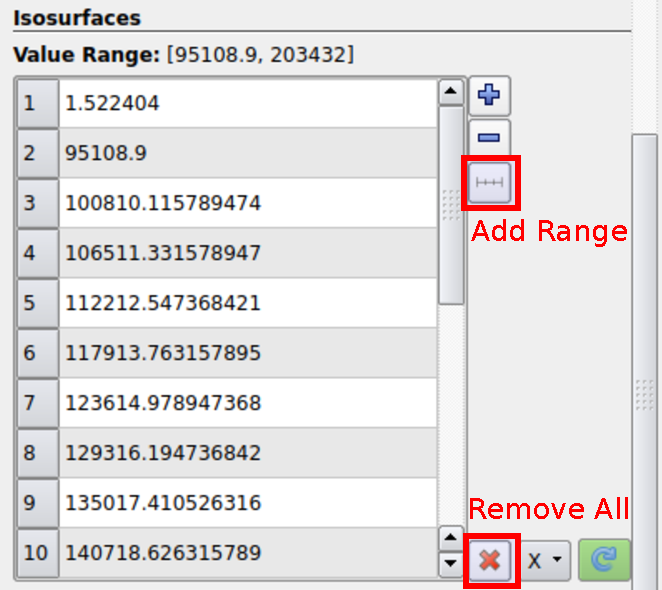
\includegraphics[width=1.0\textwidth]{tut02/deladdrange.pdf}
         \caption{Define a new contour range}
         \label{fig2:contourby2 a}
     \end{subfigure}
     \hfill
     \begin{subfigure}[b]{.4\textwidth}
         \centering
         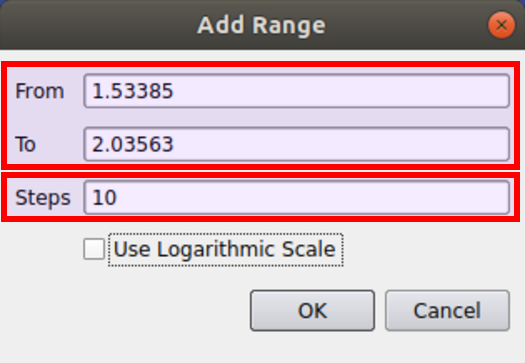
\includegraphics[width=1.0\textwidth]{tut02/addrange2.pdf}
         \caption{Add range}
         \label{fig2:contourby2 b}
     \end{subfigure}     
    \caption{Define a new range for the contour lines.}
    \label{fig2:contourby2}
\end{figure}
Now the Mach number contours should look similar to Figure \ref{fig2:mach_contour}. Additionally, if you zoom-in the plot you will see more contour details near the wedge, similar to Figure \ref{fig2:mach_contour_zoom}.
\begin{figure}[htbp]
    \centering
    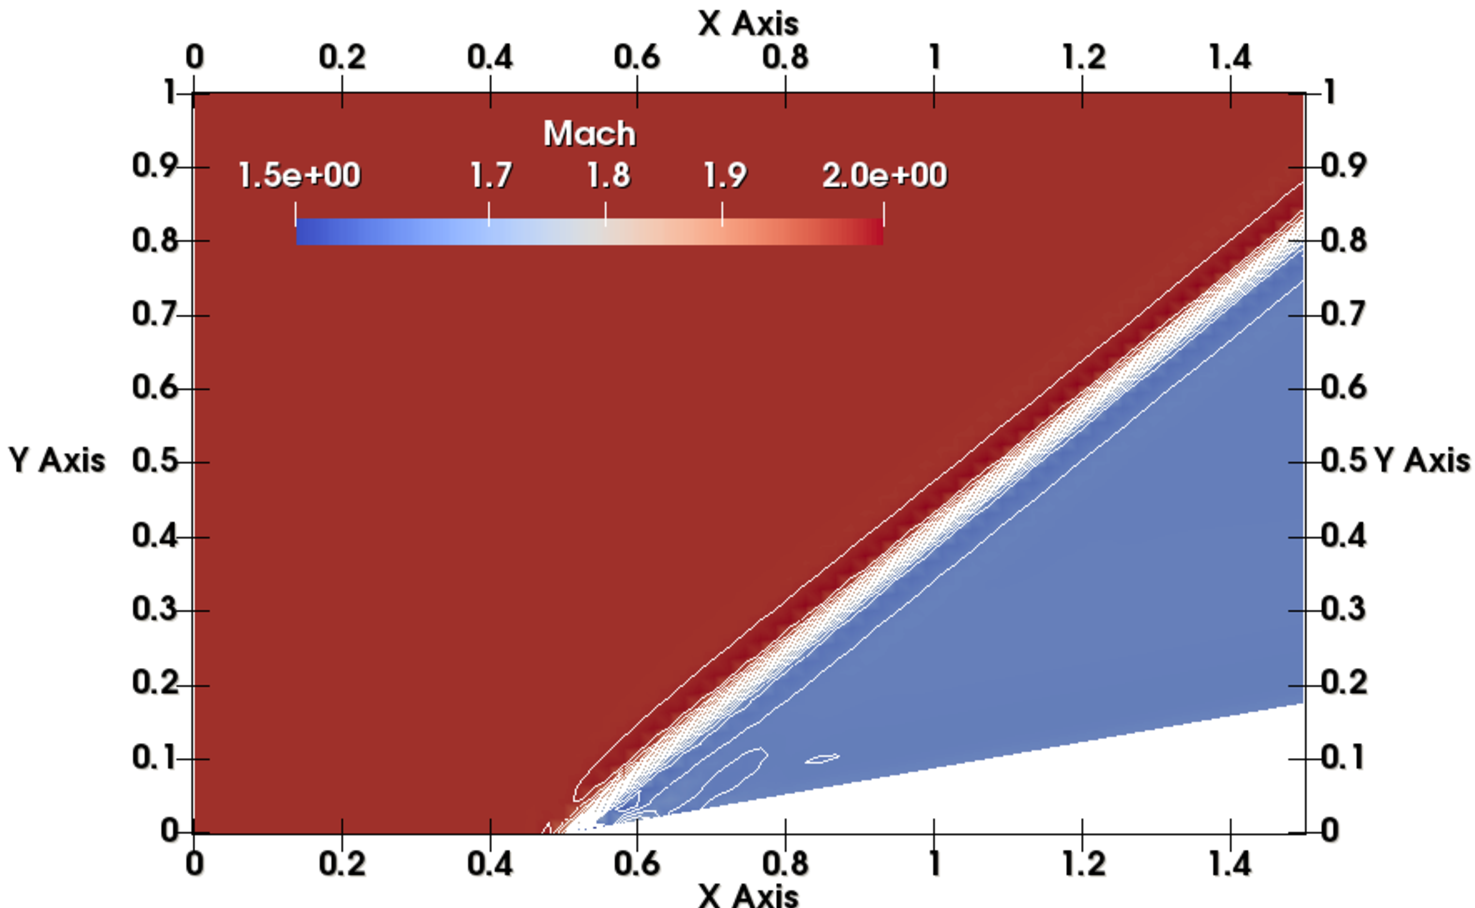
\includegraphics[width=.85\textwidth]{tut02/plot1machcont.pdf}
    \caption{Mach number contours superimposed with contour lines for the supersonic wedge case.}
    \label{fig2:mach_contour}
\end{figure}
\begin{figure}[htbp]
    \centering
    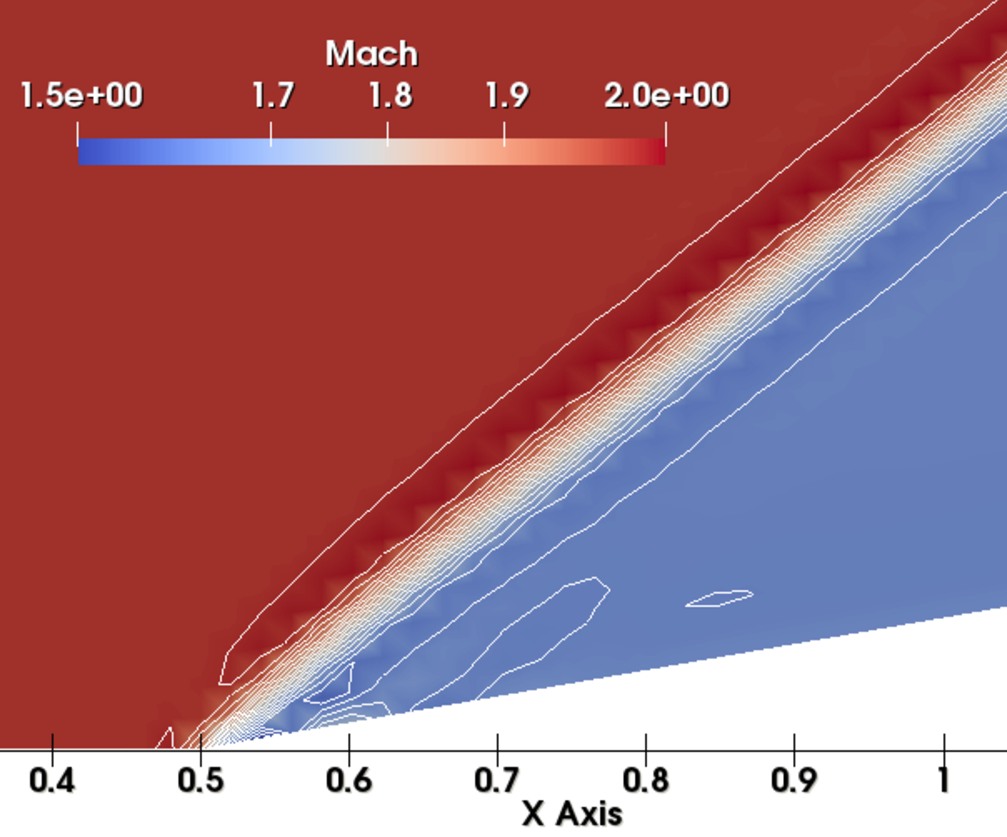
\includegraphics[width=.65\textwidth]{tut02/plot1machcont2.pdf}
    \caption{Magnified Mach number contours superimposed with contour lines for the supersonic wedge case.}
    \label{fig2:mach_contour_zoom}
\end{figure}
%--------------------------------------------------------------
\subsection{Plotting a variable over an arbitrary line}
To plot a variable over an arbitrary line in space you can select \textit{flow}.vtk by clicking on it in the \textbf{Pipeline Browser}. Next, as shown in Figure \ref{fig2:plot_over_line}, go to \textbf{Filters} $\rightarrow$  \textbf{Data Analysis} $\rightarrow$  \textbf{Plot Over Line}.
\begin{figure}[htbp]
    \centering
    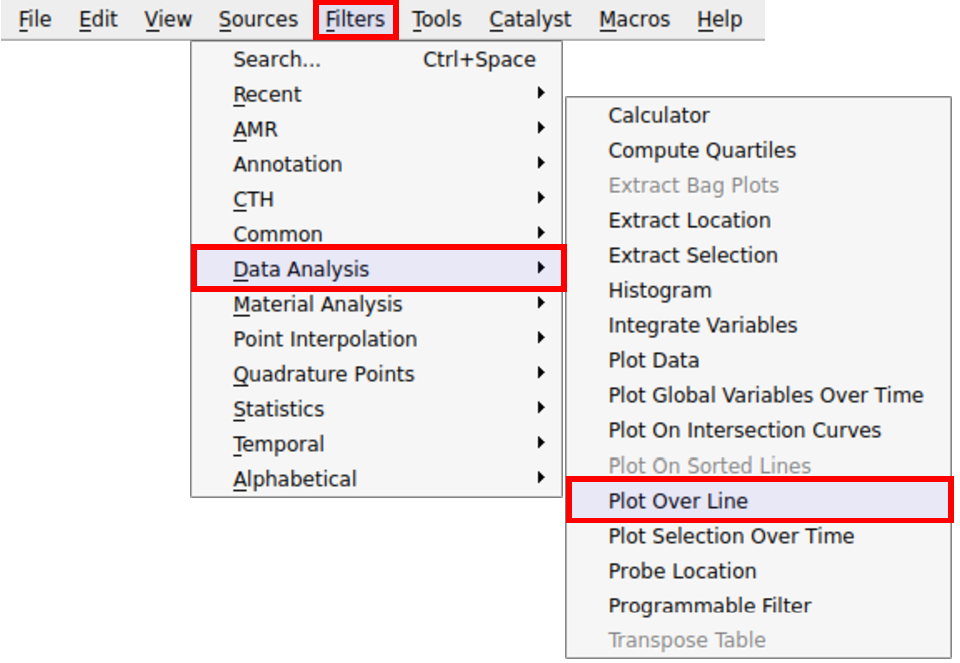
\includegraphics[width=.75\textwidth]{tut02/plotoverline.pdf}
    \caption{How to plot data over an arbitrary line in space.}
    \label{fig2:plot_over_line}
\end{figure}
Next, as shown in Figure \ref{fig2:line_coordinate}, under \textbf{Line Parameters} in \textbf{Properties}, select the coordinates for two arbitrary points you want (i.e. \textbf{Point1} and \textbf{Point2}). In this case, plot the line from \textbf{Point1} to \textbf{Point2} with (0,0.5,0) and (1.5,0.5,0), respectively, and then click \textbf{Apply}.
\begin{figure}[htbp]
    \centering
    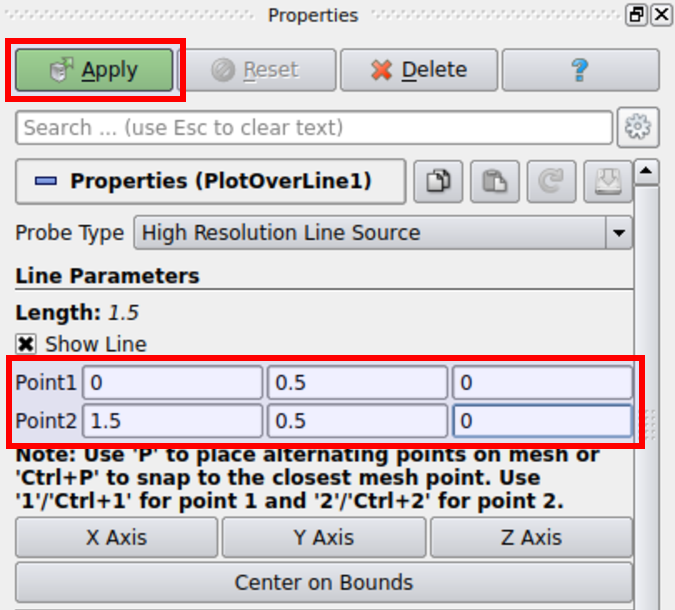
\includegraphics[width=.45\textwidth]{tut02/linecoord.pdf}
    \caption{Define the coordinates for a line plot in space.}
    \label{fig2:line_coordinate}
\end{figure}
A new line plot item will be generated. As shown in Figure \ref{fig2:plot_line_setting}, under the \textbf{X Axis Parameters} from \textbf{Display}, select \textit{Point\_X} from the \textbf{X Array Name} drop-down menu. Now, under the \textbf{Series Parameters} options toggle the box beside \textbf{Variable} to uncheck everything, then select only the \textit{Mach} item.
\begin{figure}[htbp]
    \centering
    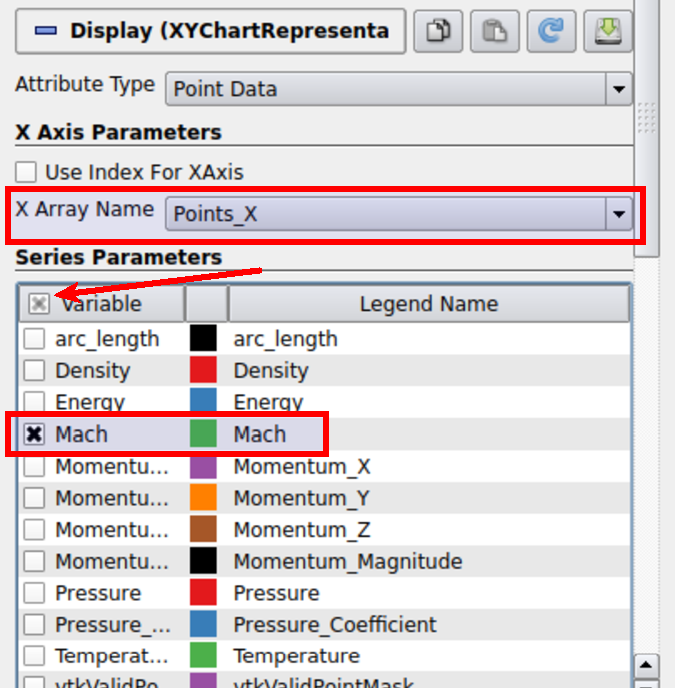
\includegraphics[width=.45\textwidth]{tut02/plotmachline.pdf}
    \caption{How to plot Mach number over a line.}
    \label{fig2:plot_line_setting}
\end{figure}
The plot of Mach number vs the \textit{x-coordinate} will be displayed in the main window as shown in Figure \ref{fig2:plot_line}.
\begin{figure}[htbp]
    \centering
    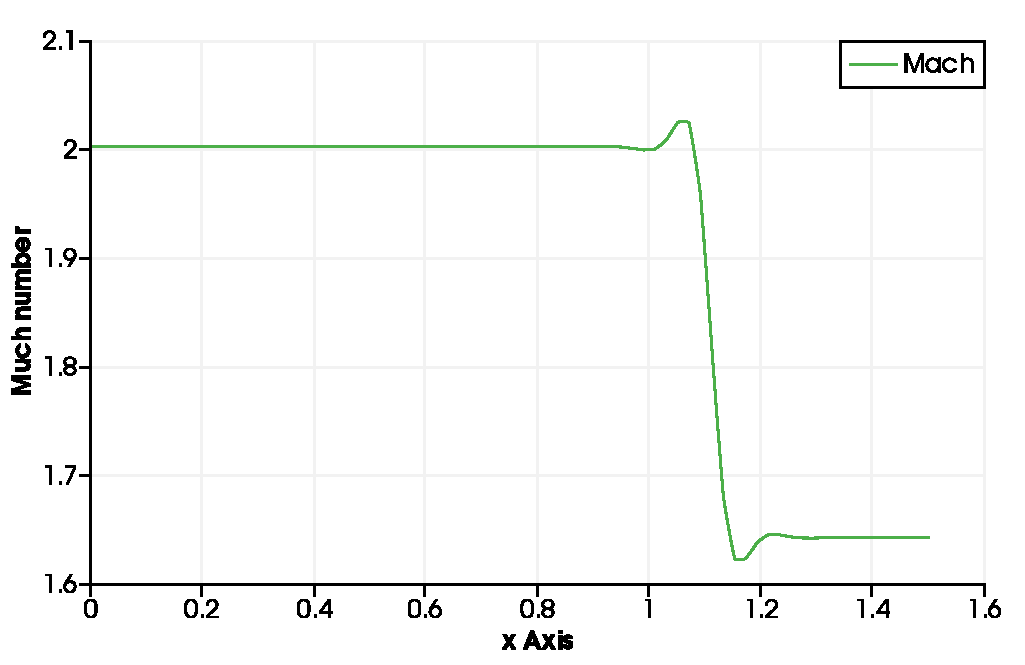
\includegraphics[width=.85\textwidth]{tut02/plot2contourline.pdf}
    \caption{Mach number plotted over the specified line.}
    \label{fig2:plot_line}
\end{figure}
In order to see a spreadsheet view of the datapoints you can click the upper right icon as shown in Figure \ref{fig2:open_spreadsheet}, then click on the \textit{Spreadsheet View} similar to Figure \ref{fig2:spreadsheet}.
\begin{figure}[htbp]
    \centering
    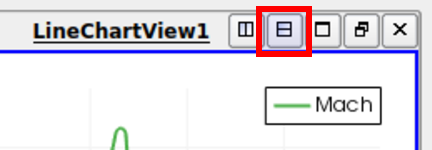
\includegraphics[width=.3\textwidth]{tut02/openspreadsheet.pdf}
    \caption{How to make spreadsheet view in a new window.}
    \label{fig2:open_spreadsheet}
\end{figure}
\begin{figure}[htbp]
    \centering
    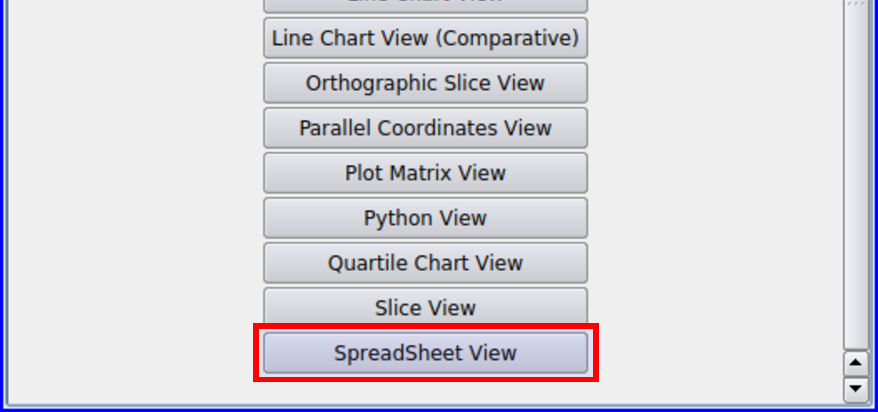
\includegraphics[width=.65\textwidth]{tut02/spreadsheet.pdf}
    \caption{Selecting the \textit{Spreadsheet View} among the different available views.}
    \label{fig2:spreadsheet}
\end{figure}
Additionally, you can export a .csv file and plot it with any other plotting software. To export the spreadsheet as a .csv file, go to \textbf{File} $\rightarrow$ \textbf{Export}, and then \textbf{Save as} .csv.
%++++++++++++++++++++++++++++++++++++++++++++++++++++++++++++++
\clearpage
\section{Questions}
1. Run the default case as provided which uses 2ND\_ORDER and the HLLC Riemann solver.
\begin{enumerate}[label=(\alph*)]
    \item Create coloured contours of Pressure and Mach number in the entire domain.
    \item Plot Pressure from (0,0.5,0) to (1.5,0.5,0) using the \textbf{Plot Over Line}.
\end{enumerate}
2. Repeat Q.1 but switch the SPATIAL\_ORDER\_FLOW to 1ST\_ORDER. \\
3. Repeat 1 using SPATIAL\_ORDER\_FLOW as 2ND\_ORDER but using the JST flux. \\
4. Repeat Q.1 using SPATIAL\_ORDER\_FLOW as 2ND\_ORDER but using the LAX-FRIEDRICH flux. \\
5. Repeat Q.1 using SPATIAL\_ORDER\_FLOW as 2ND\_ORDER but using the CUSP flux. \\
6. Repeat Q.1 using SPATIAL\_ORDER\_FLOW as 2ND\_ORDER but using the ROE flux. \\
7. Comment on how the spatial order of accuracy and choice of Riemann solver affect the resolution of the shock and any dissipation or dispersion errors you can observe. Based on your results, recommend a combination of spatial order and Riemann solver that performs particularly well.
%++++++++++++++++++++++++++++++++++++++++++++++++++++++++++++++
%++++++++++++++++++++++++++++++++++++++++++++++++++++++++++++++
%++++++++++++++++++++++++++++++++++++++++++++++++++++++++++++++
\chapter{Inviscid ONERA M6}
\label{ch:Inviscid ONERA M6}
%++++++++++++++++++++++++++++++++++++++++++++++++++++++++++++++
\section{Required Files}
\begin{su2note}
	Use the following links to download the same version of SU2 for Windows (\href{https://users.encs.concordia.ca/~bvermeir/book/executables/windows/SU2-v7.0.0-win64.zip}{\underline{click here}}) or Mac (\href{https://users.encs.concordia.ca/~bvermeir/book/executables/osx/SU2-v7.0.0-macos64.zip}{\underline{click here}}), and the required configuration (\href{https://gitlab.com/bvermeir/book-cfd/blob/master/tutorial/tut3_invisicd_oneram6/inv_ONERAM6.cfg}{\underline{click here}}) and mesh files (\href{https://gitlab.com/bvermeir/book-cfd/blob/master/tutorial/tut3_invisicd_oneram6/mesh_ONERAM6_inv.su2}{\underline{click here}}).
\end{su2note}
\begin{paraviewnote}
	Use the following links to download the same version of Paraview for Windows (\href{https://users.encs.concordia.ca/~bvermeir/book/executables/windows/ParaView-5.4.0-Qt5-OpenGL2-Windows-64bit.exe}{\underline{click here}}) or Mac (\href{https://users.encs.concordia.ca/~bvermeir/book/executables/osx/ParaView-5.4.0-Qt5-OpenGL2-MPI-OSX10.8-64bit.dmg}{\underline{click here}}).
\end{paraviewnote}

\section{Problem Description}
In this tutorial, we are going to explain how to simulate transonic inviscid flow around the three-dimensional ONERA M6 wing. This is a commonly used benchmark problem for computational aerodynamics, due to the availability of experimental data and its relatively simple geometry. In this tutorial the computational domain is discretized using an unstructured mesh with of 582,752 tetrahedral elements. The flow specification is as follows:
\begin{itemize}
    \item Pressure = 101,325 Pa
    \item Temperature = 273.15 K
    \item Mach number = 0.8395
    \item angle of attack = 3.06 degrees
\end{itemize}

This tutorial has two parts: Flow Solution and Post-processing. In the first part, we will explain how to manage the prerequisite files and settings, and how to run the CFD simulation using SU2. In the second part we explain how to use Paraview to visualize the data obtained from SU2.
%++++++++++++++++++++++++++++++++++++++++++++++++++++++++++++++
\section{Flow solution}
In the configuration file you can manually adjust the multi-grid control parameters. For the tutorial case you will see that the number of multigrid levels is set to 0, \texttt{MGLEVEL=0}. In the assigned questions the number of multigrid levels will be changed by adjusting this \texttt{MGLEVEL} parameter. You can also select the multi-grid cycle type choosing one of \texttt{MGCYCLE (V Cycle, W Cycle or Full MG Cycle)}. Another parameter of interest is the total number of iterations. This can be modified by changing the value in \texttt{EXT\_ITER}. For this example it will be kept at 200, but depending on the method used more iterations may be required to reach convergence. We will post-process the results by obtaining pressure coefficient and Mach number contours, lift coefficient ($C_L$), and drag coefficient ($C_D$) of the ONERA M6 wing. We will also explore the rate of convergence as a function of the number of multigrid levels used.

To run the simulation SU2 needs two essential files: the configuration file (.cfg) and the mesh file (.su2). Links to the required files and executables are provided at the start of this tutorial. The files include:
\begin{enumerate}
\item \textit{inv\_ONERAM6}.cfg as a configuration file.
\item \textit{mesh\_ONERAM6\_inv}.su2 as a mesh file.
\end{enumerate}
The next step is to copy these two files into the same directory as your SU2 executable. Then open a terminal window and execute the following commands to run the simulation:
\begin{table}[htbp]
    \centering
    \begin{tabular}{|l|l|}
    \hline
    Windows     & \begin{tabular}{c} \$ cd "where you saved the package" \\ \$ SU2\_CFD.exe inv\_ONERAM6.cfg \end{tabular}
    \\
    \hline
    Mac     & \begin{tabular}{c} \$ cd "where you saved the package" \\ \$ SU2\_CFD.exe inv\_ONERAM6.cfg \end{tabular}
    \\
    \hline
    \end{tabular}
\end{table}

The SU2 solver will commence solving the problem and will print out the residuals at every iteration, until the specified convergence criteria is achieved. After the calculations are complete the following output files should have been generated within in the SU2 folder:
\begin{itemize}
    \item \textit{flow}.vtk: The flow solution on the entire domain.
    \item \textit{force\_breakdown}.dat: Forces and moment on the airfoil.
    \item \textit{history}.vtk: Convergence history.
    \item \textit{restart\_flow}.dat: Restart file.
    \item \textit{surface\_flow}.vtk: The flow solution on the airfoil surface.
    \item \textit{surface\_flow}.csv: A comma separated value file of the flow solution on the airfoil.
\end{itemize}
Please keep in mind that every time you run SU2, the output data will be overwritten. Hence, before launching a new simulation you should backup your files in another directory.
%++++++++++++++++++++++++++++++++++++++++++++++++++++++++++++++
\section{Post-processing}
In this section, we will explain how to use Paraview to visualize the results produced by SU2. 
%--------------------------------------------------------------
\subsection{Load the Solution File:}
Launch Paraview. Go to \textbf{File} $\rightarrow$ \textbf{Open}, and select the \textit{surface\_flow}.vtk file. On the left-hand side of the Paraview window you will see the file is loaded under \textbf{builtin} in \textbf{Pipeline Browser}. Press the \textbf{Apply} button in the \textbf{Properties} tab, right under the \textbf{Pipeline Browser} heading. Paraview will now load the data associated with your file, and it will now be ready for visualization (Figure \ref{fig3:load}).
\begin{figure}[htbp]
    \centering
    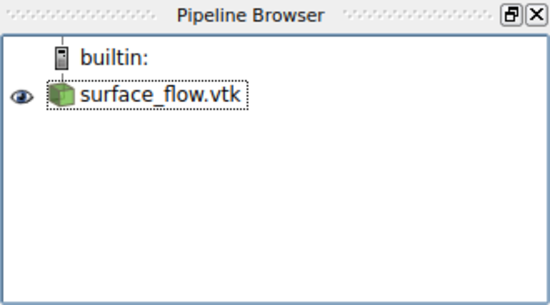
\includegraphics[width=0.4\textwidth]{tut03/surface_flow.pdf}
    \caption{Loading \textit{surface\_flow}.vtk file in the \textbf{Pipeline Browser}.}
    \label{fig3:load}
\end{figure}
%--------------------------------------------------------------
\subsection{Visualize the Mesh}
In order to view the mesh, as shown in Figure \ref{fig3:wireframe}, select \textit{Solid Color} with \textit{Wireframe} in the toolbar. As you can see in Figure \ref{fig3:mesh}, the mesh around the ONERA M6 wing is unstructured, and the elements are clustered around the wingtip, leading edge, and trailing edge of the wing. This is to accommodate large changes in the flow solution in the vicinity of the features.
\begin{figure}[htbp]
    \centering
    \includegraphics[width=0.6\textwidth]{tut03/wireframe.pdf}
    \caption{How to display mesh in computational domain.}
    \label{fig3:wireframe}
\end{figure}
\begin{figure}[htbp]
    \centering
    \includegraphics[width=.75\textwidth]{tut03/mesh2.pdf}
    \caption{Unstructured mesh around ONERA M6 wing.}
    \label{fig3:mesh}
\end{figure}
%--------------------------------------------------------------
\subsection{Visualize Pressure Coefficient Contour and Much Number Contour}
To display pressure contours on the surface of the wing click on \textit{surface\_flow}.vtk in the \textbf{Pipeline Browser}. Then click on the \textbf{Display} in \textbf{Properties} tab. Next, under \textbf{Coloring}, select \textit{Pressure\_Coefficient} from the drop-down menu (Figure \ref{fig3:pressure_coeff_1}).
\begin{figure}[htbp]
    \centering
    \includegraphics[width=0.4\textwidth]{tut03/coloring.pdf}
    \caption{Display contour by selecting variable.}
    \label{fig3:pressure_coeff_1}
\end{figure}
The pressure coefficient contour should now be displayed similar to Figure \ref{fig3:plot_pressure_coeff}
\begin{figure}[htbp]
    \centering
    \includegraphics[width=0.65\textwidth]{tut03/cont1_pressure_coefficient.pdf}
    \caption{Pressure coefficient contour for ONERA M6 wing.}
    \label{fig3:plot_pressure_coeff}
\end{figure}

To add contour lines to the plot click on \textit{surface\_flow}.vtk in the \textbf{Pipeline Browser}, and then click on the \textbf{Contour} icon (Figure \ref{fig3:contour_icon}) in the toolbar.
\begin{figure}[htbp]
    \centering
    \includegraphics[width=0.5\textwidth]{tut03/contourlineicon.pdf}
    \caption{\textbf{Contour} icon in toolbar.}
    \label{fig3:contour_icon}
\end{figure}
The \textit{Contour1} item now appears under the \textit{flow}.vtk file in the \textbf{Pipeline Browser} (Figure \ref{fig3:contour1}). Click on \textbf{Apply} to proceed to the next step.
\begin{figure}[htbp]
    \centering
    \includegraphics[width=0.4\textwidth]{tut03/contour1.pdf}
    \caption{Adding \textit{Contour1} in \textbf{Pipeline Browser}.}
    \label{fig3:contour1}
\end{figure}
As shown in Figure \ref{fig3:contourby a}, go to the \textbf{Properties}, and choose \textit{Pressure\_Coefficient} from \textbf{Contour By} drop-down menu. Then, click on the \textbf{Add Range} icon to customize the range used for the pressure contours. As shown in Figure \ref{fig3:contourby b}, set the max/min (i.e. \textbf{From}/\textbf{To}) range of contour lines, as well as the number steps used to divide this range into the equal contour levels. Set \textbf{Step} to 20, and then click on \textbf{OK}. At the end, click on \textbf{Apply} to generate the contour lines in the display window.
\begin{figure}[htbp]
    \centering
     \begin{subfigure}[b]{.4\textwidth}
         \centering
         \includegraphics[width=1.0\textwidth]{tut03/pressure_coeff_addrange1.pdf}
         \caption{Define new range}
         \label{fig3:contourby a}
     \end{subfigure}
     \hfill
     \begin{subfigure}[b]{.4\textwidth}
         \centering
         \includegraphics[width=1.0\textwidth]{tut03/pressure_coeff_addrange2.pdf}
         \caption{Add range}
         \label{fig3:contourby b}
     \end{subfigure}     
    \caption{How to define a new range for the contour lines.}
    \label{fig3:contourby}
\end{figure}
Next, as shown in Figure \ref{fig3:colorby2}, click on \textbf{Display} under the \textbf{Properties} tab. In the \textbf{Coloring} section select \textbf{Solid Color} from the drop-down menu and choose black from \textbf{Edit}.
\begin{figure}[htbp]
    \centering
    \includegraphics[width=0.4\textwidth]{tut03/coloring2.pdf}
    \caption{Changing contour lines color in \textbf{Coloring} section.}
    \label{fig3:colorby2}
\end{figure}
The pressure contours will now be displayed in black and should be similar to Figure \ref{fig3:pressure_contour_lines}.
\begin{figure}[htbp]
    \centering
    \includegraphics[width=.65\textwidth]{tut03/cont2_pressure_coefficient.pdf}
    \caption{Pressure coefficient contour superimposed by contour lines for ONERA M6 wing.}
    \label{fig3:pressure_contour_lines}
\end{figure}

To display Mach number contours, similar to Figure \ref{fig3:pressure_coeff_1}, click on \textit{surface\_flow}.vtk in the \textbf{Pipeline Browser}. Under \textbf{Coloring} from the \textbf{Display} section select \textit{Mach} from drop-down menu. Now click on "\textit{Contour1}" in the \textbf{Pipeline Browser}. As shown in Figure \ref{fig3:contourby2 a}, under the \textbf{Properties} tab, select \textit{Mach} from the \textbf{Contour By} drop-down menu. Next, click on the \textbf{Remove All} icon to remove previous the range used for the pressure coefficient. Similar to Figure \ref{fig3:contourby2 b}, click on the \textbf{Add Range} icon and set \textbf{Steps} to 20. Next, click on \textbf{OK} and \textbf{Apply} to show the plot.
\begin{figure}[htbp]
    \centering
     \begin{subfigure}[b]{.4\textwidth}
         \centering
         \includegraphics[width=1.0\textwidth]{tut03/del_add_range_mach.pdf}
         \caption{Define new range}
         \label{fig3:contourby2 a}
     \end{subfigure}
     \hfill
     \begin{subfigure}[b]{.4\textwidth}
         \centering
         \includegraphics[width=1.0\textwidth]{tut03/AddRangemach.pdf}
         \caption{Add range}
         \label{fig3:contourby2 b}
     \end{subfigure}     
    \caption{How to define a new range for the contour lines.}
    \label{fig3:contourby2}
\end{figure}
Now the Mach number contours on the wing surface should be shown, similar to Figure \ref{fig3:mach_contour}.
\begin{figure}[htbp]
    \centering
    \includegraphics[width=0.5\textwidth]{tut03/machcontour1.pdf}
    \caption{Mach number contour with superimposed by lines.}
    \label{fig3:mach_contour}
\end{figure}
%--------------------------------------------------------------
\subsection{Comparison of Convergence Rate}
We will now explore the rate of convergence of the SU2 solver. Open any suitable plotting or spreadsheet software. Open the file \textit{history}.vtk that was generated by SU2. Choose the file type that best describes your data, and tell your software to use \textit{Tab}, \textit{Semicolon}, and \textit{Comma} as delimiters (Figure \ref{fig3:importvtkxlxs}).
\begin{figure}[htbp]
    \centering
    \includegraphics[width=0.5\textwidth]{tut03/16.png}
    \caption{Import .vtk file in Microsoft Excel.}
    \label{fig3:importvtkxlxs}
\end{figure}
As shown in Figure \ref{fig3:columnsxlxs}, the first column shows the iteration number. The lift coefficient ($C_L$) and the drag coefficient ($C_D$) are displayed in the second and third columns, respectively. Finally, the residuals can also be examined to check the rate of convergence (Column \textit{L} to Column \textit{P} in Figure \ref{fig3:residualxlxs}).
\begin{figure}[htbp]
    \centering
    \includegraphics[width=0.5\textwidth]{tut03/17.png}
    \caption{Columns in \textit{history}.vtk}
    \label{fig3:columnsxlxs}
\end{figure}
\begin{figure}[htbp]
    \centering
    \includegraphics[width=0.75\textwidth]{tut03/18.png}
    \caption{Residuals in \textit{history}.vtk}
    \label{fig3:residualxlxs}
\end{figure}
Now we can plot the predicted lift coefficient, drag coefficient, and density residual against the number of iterations to see how many iterations it takes to converge to a steady solution. Figure \ref{fig3:clcdxlxs} and Figure \ref{fig3:res_vs_itr} show plots for the aerodynamic loads and residual as a function of the number of iterations, respectively, for the case of no multigrid, \texttt{MGLEVEL=0}.
\begin{figure}[htbp]
    \centering
    \includegraphics[trim=3cm 17cm 4cm 3cm, clip=true, width=0.75\textwidth]{tut03/clcd03.pdf}
    \caption{Lift and Drag coefficients versus the number of iterations.}
    \label{fig3:clcdxlxs}
\end{figure}
\begin{figure}[htbp]
    \centering
    \includegraphics[trim=3cm 17cm 4cm 3cm, clip=true, width=0.75\textwidth]{tut03/res03.pdf}
    \caption{Density residual versus the number of iterations.}
    \label{fig3:res_vs_itr}
\end{figure}
%++++++++++++++++++++++++++++++++++++++++++++++++++++++++++++++
\clearpage
\section{Questions}
1. Run the simulation without multi-grid scheme (\texttt{MGLEVEL=0}).
\begin{enumerate}[label=(\alph*)]
    \item Follow the procedure in the guideline document to run the simulation and record the number of iterations and wall-clock time for the simulation to complete.
    \item Record the lift and drag coefficients.
    \item Plot the surface pressure coefficient with coloured contours and contour lines.
    \item Plot the surface Mach number with coloured contours and contour lines.
    \item Plot the value of $C_L$, $C_D$ and the density residual vs. the number of iterations.
\end{enumerate}
2. Modify the configuration file in the multi-grid folder (\texttt{MGLEVEL= 3, MGCYCLE= W\_CYCLE}) and repeat Q.1 using multi-grid scheme.\\
3. Compare the results in part (a)-(e) of Q.1 and Q.2. In what way is the use of multi-grid advantageous for this test case?\\
%++++++++++++++++++++++++++++++++++++++++++++++++++++++++++++++
%++++++++++++++++++++++++++++++++++++++++++++++++++++++++++++++
%++++++++++++++++++++++++++++++++++++++++++++++++++++++++++++++
\chapter{Laminar Cylinder}
\label{ch:Laminar Cylinder}
%++++++++++++++++++++++++++++++++++++++++++++++++++++++++++++++
\section{Required Files}
\begin{su2note}
	Use the following links to download the same version of SU2 for Windows (\href{https://users.encs.concordia.ca/~bvermeir/book/executables/windows/SU2-v7.0.0-win64.zip}{\underline{click here}}) or Mac (\href{https://users.encs.concordia.ca/~bvermeir/book/executables/osx/SU2-v7.0.0-macos64.zip}{\underline{click here}}), and the required configuration (\href{https://gitlab.com/bvermeir/book-cfd/blob/master/tutorial/tut4_laminar_cylinder/steady/lam_cylinder.cfg}{\underline{click here}}) and mesh files (\href{https://gitlab.com/bvermeir/book-cfd/blob/master/tutorial/tut4_laminar_cylinder/steady/mesh_cylinder_lam.su2}{\underline{click here}}).
\end{su2note}
\begin{paraviewnote}
	Use the following links to download the same version of Paraview for Windows (\href{https://users.encs.concordia.ca/~bvermeir/book/executables/windows/ParaView-5.4.0-Qt5-OpenGL2-Windows-64bit.exe}{\underline{click here}}) or Mac (\href{https://users.encs.concordia.ca/~bvermeir/book/executables/osx/ParaView-5.4.0-Qt5-OpenGL2-MPI-OSX10.8-64bit.dmg}{\underline{click here}}).
\end{paraviewnote}

\section{Problem Description}
In this tutorial we will explain how to simulate external viscous flow past a 2D cylinder. To simulate this the Navier-Stokes equations will be solved in steady and unsteady forms, depending on the chosen Reynolds number. For this type of flow, the wake is expected to remain steady up to a Reynolds number of around 46. At higher Reynolds numbers the flow becomes unsteady, with oscillating vortices being shed in its wake. This is the  Von-Karman vortex street, which is a well-known phenomenon in fluid mechanics. The computational domain for this tutorial uses an O-topology mesh with the cylinder in the center of the domain. The outer boundary is situated at a radial distance of 15$D$, where $D$ is cylinder diameter. The resulting mesh is composed of 26,192 triangular elements. The elements around the surface of the cylinder are refined to resolve the viscous boundary layer in this region.  For this example, the flow specifications are provided as follows:
\begin{itemize}
    \item Pressure = 101,325Pa
    \item Temperature = 273.15K
    \item Mach number = 0.1
    \item angle of attack = 0 degrees
    \item Reynolds number = 40
    \item Characteristic length = 1m
\end{itemize}
This tutorial has two parts: Flow Solution and Post-processing. In the first part, we will explain how to manage the prerequisite files and settings, and how to run the CFD simulation using SU2. In the second part we explain how to use Paraview to visualize the data obtained from SU2.
%++++++++++++++++++++++++++++++++++++++++++++++++++++++++++++++
\section{Flow solution}
To run this simulation SU2 needs two files: a configuration file (.cfg) and a mesh file (.su2). Links to the required files and executables are provided at the start of this tutorial. The files include:
\begin{enumerate}
    \item lam\_cylinder.cfg as a configuration file.
    \item mesh\_cylinder\_lam.su2 as a mesh file.
\end{enumerate}
The next step is to copy these two files into the same directory as the SU2 executable. To run the simulation, open a terminal window and enter the following commands:
\begin{table}[htbp]
    \centering
    \begin{tabular}{|l|l|}
    \hline
    Windows     & \begin{tabular}{c} \$ cd "where you saved the package" \\ \$ SU2\_CFD.exe lam\_cylinder.cfg \end{tabular}
    \\
    \hline
    Mac     & \begin{tabular}{c} \$ cd "where you saved the package" \\ \$ SU2\_CFD.exe lam\_cylinder.cfg \end{tabular}
    \\
    \hline
    \end{tabular}
\end{table}

SU2 solver will commence solving the problem, and will print out the residuals at every iteration until the specified convergence criteria is reached. After thus, the following output files will be generated and saved in the SU2 folder:
\begin{itemize}
 \item \textit{flow}.vtk: The flow solution on the entire domain.
 \item \textit{force\_breakdown}.dat: Forces and moment on the cylinder.
 \item \textit{history}.vtk: Convergence history.
 \item \textit{restart\_flow}.dat: Restart file.
 \item \textit{surface\_flow}.vtk: The flow solution on the cylinder surface.
 \item \textit{surface\_flow}.csv: A comma separated value file of the flow solution on the cylinder.
\end{itemize}
Please keep in mind that every time you run SU2, the output data will be overwritten. Hence, before launching a new simulation you should backup your files in another directory.
%++++++++++++++++++++++++++++++++++++++++++++++++++++++++++++++
\section{Post-processing}
In this section, we explain how to use Paraview to visualize the data produced by SU2.
%--------------------------------------------------------------
\subsection{Load the Solution File:}
Launch Paraview. Go to \textbf{File} $\rightarrow$ \textbf{Open}, and then select the \textit{flow}.vtk file. On the left-hand side of the Paraview window you will see the file appear under \textbf{builtin} in the \textbf{Pipeline Browser}. Now press the \textbf{Apply} button in the \textbf{Properties} tab, directly under the \textbf{Pipeline Browser}. The solution file is now loaded by Paraview and is ready to visualize (Figure \ref{fig4:load}).
\begin{figure}[htbp]
    \centering
    \includegraphics[width=0.4\textwidth]{tut04/loadvtkfile.pdf}
    \caption{Loading \textit{flow}.vtk file in the \textbf{Pipeline Browser}.}
    \label{fig4:load}
\end{figure}
%--------------------------------------------------------------
\subsection{Visualize the Mesh}
In order to display the mesh, as shown in Figure \ref{fig4:wireframe_4}, select \textit{Solid Color} with \textit{Wireframe} in the toolbar. Then, you can zoom-in to see mesh around the surface of the cylinder, as shown in Figure \ref{fig4:mesh_4}. The mesh around the cylinder is unstructured, and the elements are clustered around the cylinder to be able to capture boundary layer and wake region properly.
\begin{figure}[htbp]
    \centering
    \includegraphics[width=0.6\textwidth]{tut04/wireframe.pdf}
    \caption{How to display mesh in computational domain.}
    \label{fig4:wireframe_4}
\end{figure}
\begin{figure}[htbp]
    \centering
    \includegraphics[width=.75\textwidth]{tut04/mesh.pdf}
    \caption{Unstructured mesh around cylinder.}
    \label{fig4:mesh_4}
\end{figure}
%--------------------------------------------------------------
\subsection{Visualize Pressure Contour and Much Number Contour}
To visualize pressure contours in the domain activate \textit{flow}.vtk by clicking on it in the \textbf{Pipeline Browser}, then go to \textbf{Display} in \textbf{Properties} tab. Under the \textbf{Coloring} section select \textit{Pressure} from the drop-down menu (Figure \ref{fig4:pressure_coloring_4}).
\begin{figure}[htbp]
    \centering
    \includegraphics[width=0.4\textwidth]{tut04/coloring_pressure.pdf}
    \caption{How to display contour by selecting variable.}
    \label{fig4:pressure_coloring_4}
\end{figure}
Contours of the pressure coefficient will now be displayed, similar to Figure \ref{fig4:pressure_plot1_4}.
\begin{figure}[htbp]
    \centering
    \includegraphics[width=0.75\textwidth]{tut04/plot1_pressure.pdf}
    \caption{Pressure coefficient contour around a cylinder.}
    \label{fig4:pressure_plot1_4}
\end{figure}
To change the color range used for pressure coefficient you can also click on \textbf{Edit} under the same \textbf{Coloring} section. In order to add contour lines to the plot, click again on the \textit{flow}.vtk file in the \textbf{Pipeline Browser}. Then click on the \textbf{Contour} icon (Figure \ref{fig4:contourline1_4}). Similar to Figure \ref{fig4:contourline2_4}, you should now see \textit{Contour1} under the \textit{flow}.vtk file in the \textbf{Pipeline Browser}. 
\begin{figure}[htbp]
    \centering
    \includegraphics[width=0.4\textwidth]{tut04/contourline.pdf}
    \caption{\textbf{Contour} icon in toolbar.}
    \label{fig4:contourline1_4}
\end{figure}
\begin{figure}[htbp]
    \centering
    \includegraphics[width=0.4\textwidth]{tut04/contourline2.pdf}
    \caption{Adding \textit{Contour1} to \textbf{Pipeline Browser}.}
    \label{fig4:contourline2_4}
\end{figure}
As shown in Figure \ref{fig4:contourby_4 a}, in the \textbf{Properties} select \textit{Pressure} from the \textbf{Contour By} drop-down menu. You can use the \textbf{Remove All} icon to remove the default range, and then, click on the \textbf{Add Range} icon to make a new range based on your preference. Similar to Figure \ref{fig4:contourby_4 b}, set the \textbf{Steps} to 20, and then, click on \textbf{OK} and \textbf{Apply}, respectively.
\begin{figure}[htbp]
    \centering
    \begin{subfigure}[b]{.4\textwidth}
        \centering
        \includegraphics[width=1.0\textwidth]{tut04/contourline3.pdf}
        \caption{Define new range}
        \label{fig4:contourby_4 a}
    \end{subfigure}
    \hfill
    \begin{subfigure}[b]{.4\textwidth}
        \centering
        \includegraphics[width=1.0\textwidth]{tut04/contourline4.pdf}
        \caption{Add range}
        \label{fig4:contourby_4 b}
    \end{subfigure}     
    \caption{How to define a new range for the contour lines.}
    \label{fig4:contourby_4}
\end{figure}

To change the color of the contour lines activate \textit{Contour1} by clicking on it in \textbf{Pipeline Browser}. Then, similar to Figure \ref{fig4:pressure_coloring_4}, you can go to \textbf{Edit} under the \textbf{Coloring} section and select white. Finally, the pressure contours superimposed with appropriate contour lines should be visible, similar to Figure \ref{fig4:contourline6_4}
\begin{figure}[htbp]
    \centering
    \includegraphics[width=0.75\textwidth]{tut04/contourline6.pdf}.
    \caption{Pressure contour superimposed by contour lines around a cylinder.}
    \label{fig4:contourline6_4}
\end{figure}
Keep in mind that to display both contour and contour lines, the eye beside each iten in the \textbf{Pipeline Browser} should be activated (Figure \ref{fig4:contourline5_4})
\begin{figure}[htbp]
    \centering
    \includegraphics[width=0.4\textwidth]{tut04/contourline5.pdf}.
    \caption{How to display contour and contourlines at the same time in plot.}
    \label{fig4:contourline5_4}
\end{figure}

To display the Mach number contours click on \textit{flow}.vtk again in the \textbf{Pipeline Browser}. As shown in Figure \ref{fig4:mach1_4}, under \textbf{Coloring} section in \textbf{Display}, select \textit{Mach} from the drop-down menu.
\begin{figure}[htbp]
    \centering
    \includegraphics[width=0.4\textwidth]{tut04/mach1.pdf}.
    \caption{How to change color for contour lines of Mach number.}
    \label{fig4:mach1_4}
\end{figure}
Click on \textit{Contour1} in the \textbf{Pipeline Browser}. Similar to Figure \ref{fig4:mach2_4 a}, in \textbf{Properties} select \textit{Mach} from the \textbf{Contour By} drop-down menu. Click on \textbf{Remove All} to remove the previous value range used for pressure. Click on \textbf{Add Range} and set the the value of \textbf{Steps} to 20. Then, click \textbf{OK} and \textbf{Apply}, respectively (Figure \ref{fig4:mach2_4 b}).
\begin{figure}[htbp]
    \centering
    \begin{subfigure}[b]{0.4\textwidth}
        \centering
        \includegraphics[width=1.0\textwidth]{tut04/mach2.pdf}
        \caption{Define new range}
        \label{fig4:mach2_4 a}
    \end{subfigure}
    \hfill
    \begin{subfigure}[b]{.4\textwidth}
        \centering
        \includegraphics[width=1.0\textwidth]{tut04/mach3.pdf}
        \caption{Add range}
        \label{fig4:mach2_4 b}
    \end{subfigure}     
    \caption{How to define a new range for the contour lines.}
    \label{fig4:mach2_4}
\end{figure}
Mach number contours around the cylinder should now be visible, similar to Figure \ref{fig4:mach5_4}.
\begin{figure}[htbp]
    \centering
    \includegraphics[width=0.85\textwidth]{tut04/mach5.pdf}
    \caption{Mach number contour with superimposed by lines.}
    \label{fig4:mach5_4}
\end{figure}
%--------------------------------------------------------------
\subsection{Streamlines and Separation Length}
Streamlines show the path that a fluid element will follow, when released. Streamlines can help with visualizing flow separation and the wake region behind bluff bodies, such as the cylinder used in this tutorial. In this case, streamlines can be used to visualize the separation bubble behind the cylinder. Activate \textit{flow}.vtk by clicking on it in the \textbf{Pipeline Browser}. As shown in Figure \ref{fig4:stream1_4}, click on the \textbf{Calculator} icon, which allows you to define new variables and add add them to the list of variables.
\begin{figure}[htbp]
    \centering
    \includegraphics[width=0.4\textwidth]{tut04/stream1.pdf}
    \caption{How to define new variable using \textbf{Calculator}.}
    \label{fig4:stream1_4}
\end{figure}
Next, click on the \textit{Calculator1} in the \textbf{Pipeline Browser}, and as shown in Figure \ref{fig4:stream3_4}, rename the \textbf{Result Array Name} as \textit{Velocity}. Furthermore, following Figure \ref{fig4:stream3_4}, write the contribution of each velocity component in the equation box. Keep in mind that dividing Momentum by Density results the corresponding fluid velocity component. Then, click on \textbf{Apply} to proceed to the next step.
\begin{figure}[htbp]
    \centering
    \includegraphics[width=0.4\textwidth]{tut04/stream3.pdf}
    \caption{How to use \textbf{Calculator} to define velocity.}
    \label{fig4:stream3_4}
\end{figure}
As shown in Figure \ref{fig4:stream4_4}, \textit{Calculator1} now appears in the \textbf{Pipeline Browser} as a subset of \textit{flow}.vtk.
\begin{figure}[htbp]
    \centering
    \includegraphics[width=0.4\textwidth]{tut04/stream4.pdf}
    \caption{\textit{Calculator1} as a subset of \textit{flow}.vtk in \textbf{Pipeline Browser}.}
    \label{fig4:stream4_4}
\end{figure}
Now click again on \textit{Calculator1} in the \textbf{Pipeline Browser}, and then click on the \textbf{Stream Tracer} icon in the toolbar (Figure \ref{fig4:stream5_4}).
\begin{figure}[htbp]
    \centering
    \includegraphics[width=0.5\textwidth]{tut04/stream5.pdf}
    \caption{How to add streamlines using \textbf{Stream Tracer}.}
    \label{fig4:stream5_4}
\end{figure}
Next, click on \textit{StreamTracer1} in the \textbf{Pipeline Browser}, and as shown in Figure \ref{fig4:stream6_4}, in the \textbf{Properties} menu select \textit{Velocity} from \textbf{Vectors} drop-down menu. Additionally, select \textit{High Resolution Line Source} from the \textbf{Seed Type} drop-down menu. Now, under \textbf{Line Parameters}, set \textbf{Point1} and \textbf{Point2} as (-15,0,0) and (15,0,0), respectively. These two points define the endpoints of a line along which streamlines will be generated.  
\begin{figure}[htbp]
    \centering
    \includegraphics[width=0.4\textwidth]{tut04/stream6.pdf}
    \caption{Streamline setting in \textbf{Stream Tracer} panel.}
    \label{fig4:stream6_4}
\end{figure}
As shown in Figure \ref{fig4:stream7_4}, under \textbf{Coloring} in the \textbf{Display} section select \textit{Solid Color} from \textbf{Edit}, and then choose white for the stream lines. Additionally, click on the check-box beside \textbf{Data Axis Grid} to display the axis range in plot.
\begin{figure}[htbp]
    \centering
    \includegraphics[width=0.4\textwidth]{tut04/stream7.pdf}
    \caption{Changing stream line's color in \textbf{Display} panel.}
    \label{fig4:stream7_4}
\end{figure}
Next, hide all items except \textit{flow}.vtk and \textit{StreamTracer1} by deactivating the eye icon beside each of them (Figure \ref{fig4:stream8_4}).
\begin{figure}[htbp]
    \centering
    \includegraphics[width=0.4\textwidth]{tut04/stream8.pdf}
    \caption{Activating both \textit{flow}.vtk and \textit{StreamTracer1} in \textbf{Pipeline Browser}.}
    \label{fig4:stream8_4}
\end{figure}
Finally, Figure \ref{fig4:stream9_4} shows the Mach number contours with the streamlines superimposed on top of them. As mentioned previously, the diameter of cylinder is taken to be 1m. From Figure \ref{fig4:stream9_4} you can approximate the separation length to be around 2m behind the cylinder at the chosen $Re=40$.
\begin{figure}[htbp]
    \centering
    \includegraphics[width=0.75\textwidth]{tut04/stream9.pdf}
    \caption{Mach number contour superimposed with streamlines.}
    \label{fig4:stream9_4}
\end{figure}

The length of the separated bubble can also be calculated more precisely. To do this we will plot the streamwise velocity component along the computational domain center-line, and measure the length of the separated bubble, which is defined as the region of reversed flow in the wake. Therefore, the separation bubble length can be found as the distance between the surface of the cylinder and the location where the \textit{Velocity\_X} switches from negative to positive. To get started, in the \textbf{Pipeline Browser} click on \textit{Calculator1} and then go to the \textbf{Filters} $\rightarrow$ \textbf{Data Analysis} $\rightarrow$ \textbf{Plot Over Line} option (Figure \ref{fig4:stream10_4}).
\begin{figure}[htbp]
    \centering
    \includegraphics[width=0.55\textwidth]{tut04/stream10.pdf}
    \caption{How to plot over an arbitrary line.}
    \label{fig4:stream10_4}
\end{figure}
Now, activate \textit{PlotOverLine1} by clicking on it in the \textbf{Pipeline Browser}. As shown in Figure \ref{fig4:stream11_4}, under \textbf{Line Parameters} in the \textbf{Properties} menu set \textbf{Point1} and \textbf{Point2} as (-15,0,0) and (15,0,0), respectively. Please note that this line is different from previous line we defined to generate streamlines. Set the \textbf{Resolution} to 10,000, and then click on \textbf{Apply}.
\begin{figure}[htbp]
    \centering
    \includegraphics[width=0.4\textwidth]{tut04/stream11.pdf}
    \caption{Settings for \textbf{Plot Over Line}.}
    \label{fig4:stream11_4}
\end{figure}
As shown in Figure \ref{fig4:stream12_4}, in the \textbf{Display} panel select \textit{Point\_X} from the \textbf{X Array Name} drop-down menu. Under \textbf{Series Parameters} unselect all variables except for \textit{Velocity\_X}.
\begin{figure}[htbp]
    \centering
    \includegraphics[width=0.4\textwidth]{tut04/stream12.pdf}
    \caption{How to Plot \textit{Velocity\_X} versus \textit{X Axis}.}
    \label{fig4:stream12_4}
\end{figure}
An figure similar to Figure \ref{fig4:stream14_4} will now display the velocity profile over the chosen line along the (\textit{X Axis}). As shown in Figure \ref{fig4:stream14_4}, the separation length, $L$, can be measured when \textit{Velocity\_X} approaches zero in the wake of the cylinder.
\begin{figure}[htbp]
    \centering
    \includegraphics[width=0.95\textwidth]{tut04/stream14.pdf}
    \caption{\textit{Velocity\_X} versus \textit{X Axis}, and the length of flow separation.}
    \label{fig4:stream14_4}
\end{figure}
%--------------------------------------------------------------
\subsection{Shedding Frequency}
When the Reynolds number is high enough the wake behind the cylinder becomes unstable, and vortex shedding occurs. The frequency of the wake oscillations is called the "shedding frequency". To explore this unsteady case open the \textit{history}.vtk in an appropriate plotting program. As shown in Figure \ref{fig4:time_history}, the first column in the file shows the number of iterations. Note that the physical time can be computed by multiplying the iteration number with the time-step size, which is $\Delta t = 0.001$s for the unsteady case as set in the configuration file.
\begin{figure}[htbp]
    \centering
    \includegraphics[width=0.95\textwidth]{tut04/26.png}
    \caption{Time history of variables.}
    \label{fig4:time_history}
\end{figure}
Plotting $C_L$ or $C_D$ as a function of time demonstrates that the shedding amplitude grows, and then remains quasi-steady. The non-dimensional Strouhal number of this vortex shedding can now calculated from $St=\frac{f D}{U}$, where $f$, $D$ and $U$ are shedding frequency, cylinder diameter, and free-stream velocity, respectively. The shedding frequency can be found manually by determining the time interval between vortex shedding events in the $C_L$ time history, within the quasi-steady region.
\clearpage
%++++++++++++++++++++++++++++++++++++++++++++++++++++++++++++++
\section{Questions}
1. Run the laminar flow over a cylinder as per the tutorial case but with $Re$ = 10, 20, and 40.
\begin{enumerate}[label=(\alph*)]
    \item Plot Mach contours with streamlines for $Re$ = 10, 20, and 40
    \item Plot the $x$-velocity component vs the $x$-coordinate beginning at $x = 1$ (location of rear surface of cylinder)
    \item Calculate the $L/D$ (non-dimensional separation length) for the three Re cases and compare with the experimental $L/D$ values\cite{coutanceau1977experimental} (download \href{https://gitlab.com/bvermeir/book-cfd/blob/master/tutorial/tut4_laminar_cylinder/experimental_values.zip}{\underline{here}}). Also include the $C_D$ values for the three $Re$ cases from the simulation results. Comment on the effect of $Re$ on the non-dimensional separation length $L/D$ and $C_D$.
\end{enumerate}
2. Download configuration (\href{https://gitlab.com/bvermeir/book-cfd/blob/master/tutorial/tut4_laminar_cylinder/unsteady/lam_cylinder_re150_unsteady.cfg}{\underline{click here}}) and mesh (\href{https://gitlab.com/bvermeir/book-cfd/blob/master/tutorial/tut4_laminar_cylinder/unsteady/mesh_cylinder_lam.su2}{\underline{click here}}) files, and run an unsteady simulation for $Re$ = 150.
\begin{enumerate}[label=(\alph*)]
    \item Plot the $C_L$ and $C_D$ versus time.
    \item Calculate the $\Delta C_L$ , $\Delta C_D$ and Strouhal number, and compare your results with experimental values\cite{inoue2002sound}.
\end{enumerate}
%++++++++++++++++++++++++++++++++++++++++++++++++++++++++++++++
%++++++++++++++++++++++++++++++++++++++++++++++++++++++++++++++
%++++++++++++++++++++++++++++++++++++++++++++++++++++++++++++++
\chapter{Turbulent ONERA M6}
\label{ch:Turbulent ONERA M6}
%++++++++++++++++++++++++++++++++++++++++++++++++++++++++++++++
\section{Required Files}
\begin{su2note}
	Use the following links to download the same version of SU2 for Windows (\href{https://users.encs.concordia.ca/~bvermeir/book/executables/windows/SU2-v7.0.0-win64.zip}{\underline{click here}}) or Mac (\href{https://users.encs.concordia.ca/~bvermeir/book/executables/osx/SU2-v7.0.0-macos64.zip}{\underline{click here}}), and the required configuration (\href{https://gitlab.com/bvermeir/book-cfd/blob/master/tutorial/tut5_turbulent_oneram6/turb_ONERAM6.cfg}{\underline{click here}}) and mesh files (\href{https://gitlab.com/bvermeir/book-cfd/blob/master/tutorial/tut5_turbulent_oneram6/mesh_ONERAM6_turb_hexa_43008.su2}{\underline{click here}}).
\end{su2note}
\begin{paraviewnote}
	Use the following links to download the same version of Paraview for Windows (\href{https://users.encs.concordia.ca/~bvermeir/book/executables/windows/ParaView-5.4.0-Qt5-OpenGL2-Windows-64bit.exe}{\underline{click here}}) or Mac (\href{https://users.encs.concordia.ca/~bvermeir/book/executables/osx/ParaView-5.4.0-Qt5-OpenGL2-MPI-OSX10.8-64bit.dmg}{\underline{click here}}).
\end{paraviewnote}

\section{Problem Description}
In this tutorial will demonstrate how to simulate transonic viscous flow past a three-dimensional wing. We will use the ONERA M6 again, and detailed information is given in the previous tutorial for inviscid flow in Chapter\ref{ch:Inviscid ONERA M6}. We will use the Reynolds-Averaged Navier-Stokes (RANS) equations and compare the Spalar-Almaras (SA) and $k-\omega$ Shear Stress Transport (SST) turbulence models for the eddy viscosity. The computational domain uses a structured mesh with 43,008 hexahedral. Note that this mesh is relatively coarse to allow for relatively small computation mesh. The flow specifications are provided as follows:
\begin{itemize}
    \item Temperature = 288.15 K
    \item Mach number = 0.8395
    \item Angle of attack = 3.06 degrees
    \item Reynolds length = 0.64607 m
\end{itemize}
This tutorial has two parts: Flow Solution and Post-processing. In the first part we will explain how to manage the prerequisite files and settings, and how to run the CFD simulation using SU2. In the second part we explain how to use Paraview to visualize the data obtained from SU2.
%++++++++++++++++++++++++++++++++++++++++++++++++++++++++++++++
\section{Flow solution}
To run this simulation SU2 needs two files: a configuration file (.cfg) and a mesh file (.su2). Links to the required files and executables are provided at the start of this tutorial. The files include:
\begin{enumerate}
\item \textit{turb\_ONERAM6}.cfg as a configuration file.
\item \textit{mesh\_ONERAM6\_turb\_hexa\_43008}.su2 as a mesh file.
\end{enumerate}
The next step is to copy these two files into the same directory as the SU2 executable. To run the simulation, open a terminal window and enter the following commands:
\begin{table}[htbp]
    \centering
    \begin{tabular}{|l|l|}
    \hline
    Windows     & \begin{tabular}{c} \$ cd "where you saved the package" \\ \$ SU2\_CFD.exe turb\_ONERAM6.cfg \end{tabular}
    \\
    \hline
    Mac     & \begin{tabular}{c} \$ cd "where you saved the package" \\ \$ SU2\_CFD.exe turb\_ONERAM6.cfg \end{tabular}
    \\
    \hline
    \end{tabular}
\end{table}

SU2 solver will begin solving the problem and will print out the residuals at every iteration until the specified convergence criteria is reached. After this, the following output files should be generated and saved in the SU2 folder:
\begin{itemize}
 \item \textit{flow}.vtk: The flow solution on the entire domain.
 \item \textit{force\_breakdown}.dat: Forces and moment on the wing.
 \item \textit{history}.vtk: Convergence history.
 \item \textit{restart\_flow}.dat: Restart file.
 \item \textit{surface\_flow}.vtk: The flow solution on the wing surface.
 \item \textit{surface\_flow}.csv: A comma separated value file of the flow solution on the wing.
\end{itemize}
Please keep in mind that every time you run SU2, the output data will be overwritten. Hence, before launching a new simulation you should backup your files in another directory.
%++++++++++++++++++++++++++++++++++++++++++++++++++++++++++++++
\section{Post-processing}
In this section we demonstrate how to use Paraview to visualize the data produced by SU2.
%--------------------------------------------------------------
\subsection{Load the Solution File:}
Launch Paraview. Go to \textbf{File} $\rightarrow$ \textbf{Open}, and then select the \textit{surface\_flow}.vtk file. On the left-hand side of the Paraview window you will see the file appear under \textbf{builtin} in the \textbf{Pipeline Browser}. Now press \textbf{Apply} in the \textbf{Properties} tab under the  \textbf{Pipeline Browser}. The data file is now loaded by Paraview and is ready to visualize (Figure \ref{fig5:load}).
\begin{figure}[htbp]
    \centering
    \includegraphics[width=0.4\textwidth]{tut05/loakvtk5.png}
    \caption{Loading \textit{surface\_flow}.vtk file in the \textbf{Pipeline Browser}.}
    \label{fig5:load}
\end{figure}
%--------------------------------------------------------------
\subsection{Visualize the Mesh}
In order to view the mesh, as shown in Figure \ref{fig5:wireframe}, select \textit{Solid Color} with \textit{Wireframe} in the toolbar. Then, you can zoom-in to see mesh around the airfoil, as shown in Figure \ref{fig5:mesh}. You can see that this mesh uses structured elements, and is highly refined in the boundary layer, leading edge, and trailing edge regions.
\begin{figure}[htbp]
    \centering
    \includegraphics[width=0.75\textwidth]{tut05/wireframe.pdf}
    \caption{How to display mesh in computational domain.}
    \label{fig5:wireframe}
\end{figure}
\begin{figure}[htbp]
    \centering
    \includegraphics[trim=0.1cm 5cm 0.1cm 3cm, clip=true, width=.75\textwidth]{tut05/meshb.pdf}
    \caption{Structured mesh for ONERA M6 wing. The mesh around the surface is refined to capture the boundary layer.}
    \label{fig5:mesh}
\end{figure}
%--------------------------------------------------------------
\subsection{Visualize Pressure Coefficient at Different Stations}
In this section, we will explain how to plot the pressure coefficient on the surface of the wing as a function of chord-wise position at different span-wise stations along the wing. To get started, activate \textit{surface\_flow}.vtk by clicking on it in the \textbf{Pipeline Browser}, and then click on the \textbf{Slice} icon in the toolbar, as shown in Figure \ref{fig5:slice1}.
\begin{figure}[htbp]
    \centering
    \includegraphics[width=.6\textwidth]{tut05/slice1.pdf}
    \caption{How to slice a 3D computational domain.}
    \label{fig5:slice1}
\end{figure}
This will allow you to slice a plane through the wing, to plot the pressure coefficient ($C_p$) at a specific station
or location along the span. As shown in Figure \ref{fig5:slice2}, click on \textit{Y Normal}, and under \textbf{Plane Parameters} specify the $y$-coordinate location in the \textbf{Origin} field where we want the slice to be taken. For this example we select (0.5705415, 0.6081815, 0) as a suitable value for \textbf{Origin}, which is approximately in the middle of the wing (Figure \ref{fig5:slice3}). Click on \textbf{Apply} after specifying the $y$-coordinate.
\begin{figure}[htbp]
    \centering
    \includegraphics[width=.45\textwidth]{tut05/slice2.pdf}
    \caption{Setting for \textbf{Slice} in \textbf{Properties} panel.}
    \label{fig5:slice2}
\end{figure}
\begin{figure}[htbp]
    \centering
    \includegraphics[width=.55\textwidth]{tut05/slice3.pdf}
    \caption{Determining the slice to be taken (red line shows the location where a cross-sectional slice will be taken form the wing).}
    \label{fig5:slice3}
\end{figure}
After clicking on the \textbf{Apply}, you will generate a slice of the wing span at the specified $y$-coordinate, as shown in Figure \ref{fig5:slice4}.
\begin{figure}[htbp]
    \centering
    \includegraphics[width=.75\textwidth]{tut05/slice4.pdf}
    \caption{Slice to be taken form the wing.}
    \label{fig5:slice4}
\end{figure}
To plot $C_p$ along this slice the chord line should first be made non-dimensional. To do this, click on the upper left icon, as shown in Figure \ref{fig5:toprighticon}.
\begin{figure}[htbp]
    \centering
    \includegraphics[width=.35\textwidth]{tut05/toprighticon.pdf}
    \caption{How to make alternative viewing options.}
    \label{fig5:toprighticon}
\end{figure}
This will create another set of viewing options. By click on the \textit{Spreadsheet View}, as shown in Figure \ref{fig5:slice6}, it will generate a spreadsheet view of the data contained in that slice. As seen from Figure \ref{fig5:slice7}, we want to pan to the right where the data set of \textbf{Points} are located. You can vary the display \textbf{Precision} when looking up the maximum and minimum values as well.
\begin{figure}[htbp]
    \centering
    \includegraphics[width=.55\textwidth]{tut05/slice6.pdf}
    \caption{How to make spreadsheet view.}
    \label{fig5:slice6}
\end{figure}
Double click on the \textbf{Points} to sort them by descending or ascending order. We want to get the maximum and minimum values in the array to determine the local chord length on the wing. As shown in Figure \ref{fig5:slice7 a} and Figure \ref{fig5:slice7 b}, the maximum and minimum values for this slice are 0.97631m and 0.349704m, respectively. These two values correspond to $x$-coordinate for the trailing edge and leading edge of the chosen wing section, respectively. As you can see in Figure \ref{fig5:slice7}, the $y$-coordinate is constant for all values, our slice was taken perpendicular to the $y$-coordinate.
\begin{figure}[htbp]
    \centering
     \begin{subfigure}[b]{.85\textwidth}
         \centering
         \includegraphics[width=1.0\textwidth]{tut05/slice7a.pdf}
         \caption{Maximum value for $x$-component of the \textbf{Points}.}
         \label{fig5:slice7 a}
     \end{subfigure}
     \hfill
     \begin{subfigure}[b]{.85\textwidth}
         \centering
         \includegraphics[width=1.0\textwidth]{tut05/slice7b.pdf}
         \caption{Minimum value for $x$-component of the \textbf{Points}.}
         \label{fig5:slice7 b}
     \end{subfigure}     
    \caption{How to find maximum/minimum of the \textbf{Points}.}
    \label{fig5:slice7}
\end{figure}
Next, click on \textit{Slice1} in the \textbf{Pipeline Browser}, and click on the \textbf{Calculator} icon (Figure \ref{fig5:slice8}).
\begin{figure}[htbp]
    \centering
    \includegraphics[width=.55\textwidth]{tut05/slice8.pdf}
    \caption{How to use \textbf{Calculator}.}
    \label{fig5:slice8}
\end{figure}
We want to create a new array field called \textit{Normalized chord}. We will then plot the pressure coefficient ($C_p$) along the local normalized chord length. Therefore, as shown in to Figure \ref{fig5:slice9}, type \textit{Normalized chord} in the \textbf{Result Array Name} text-box. Additionally, type the following equation in the equation-box to normalize the local chord length at that chosen station along the wing span. Please note that the variable \textit{coordsX} can be chosen from the \textbf{Scalars} drop-down menu. Then, click on \textbf{Apply} to proceed the next step.
\begin{figure}[htbp]
    \centering
    \includegraphics[width=.55\textwidth]{tut05/slice9.pdf}
    \caption{How to make new variable using \textbf{Calculator}.}
    \label{fig5:slice9}
\end{figure}
After taking this step, the \textit{Normalized chord} is made and added to the list of variables that are available for plotting. You can see \textit{Normalized chord} in \textit{Spreadsheet View}, as shown in Figure \ref{fig5:slice10}.
\begin{figure}[htbp]
    \centering
    \includegraphics[width=.95\textwidth]{tut05/slice10.pdf}
    \caption{Normalized coordinate in \textit{Spreadsheet View}.}
    \label{fig5:slice10}
\end{figure}

In order to plot the pressure coefficient, activate \textit{Calculator1} by clicking on it in \textbf{Pipeline Browser} and then go to \textbf{Filter} $\rightarrow$ \textbf{Data Analysis} $\rightarrow$ \textbf{Plot Data} (Figure \ref{fig5:plotdata5}).
\begin{figure}[htbp]
    \centering
    \includegraphics[width=.65\textwidth]{tut05/plotdata.pdf}
    \caption{How to plot data versus a variable list.}
    \label{fig5:plotdata5}
\end{figure}
Consequently, \textit{PlotData1} is created and added to the \textbf{Pipeline Browser} (Figure \ref{fig5:slice11}).
\begin{figure}[htbp]
    \centering
    \includegraphics[width=.45\textwidth]{tut05/slice11.pdf}
    \caption{\textit{PlotData1} in \textbf{Pipeline Browser}.}
    \label{fig5:slice11}
\end{figure}

In the \textbf{Properties} tab, click on the \textbf{Display} panel. Next, under the \textbf{X Axis Parameters} uncheck \textbf{Use Index For XAxis}, and then choose \textit{Normalized chord} from the \textbf{X Array Name} drop-down menu. Next, unselect everything in the \textbf{Series Parameters} fields except for the \textit{Pressure\_Coefficient}. 
\begin{figure}[htbp]
    \centering
    \includegraphics[width=.55\textwidth]{tut05/slice13.pdf}
    \caption{How to plot pressure coefficient versus \textit{Normalized chord}.}
    \label{fig5:slice13}
\end{figure}
Additionally, at the bottom of the \textbf{Series Parameters} field select \textit{Diamond} for the \textbf{Marker Style}. After taking these steps, a plot for pressure coefficient should be generated, similar to Figure \ref{fig5:slice14}.
\begin{figure}[htbp]
    \centering
    \includegraphics[width=.95\textwidth]{tut05/slice14.pdf}
    \caption{Pressure coefficient on the surface of the airfoil versus \textit{Normalized chord}.}
    \label{fig5:slice14}
\end{figure}
Similar to the inviscid tutorial, we want to have the $C_p$ on the suction surface to be on top of the pressure side. To do this, go to the \textbf{Properties} tab and select the \textbf{View} panel. As shown in Figure \ref{fig5:slice16}, under \textbf{Left Axis Range} you can click on the check-box beside the \textbf{Left Axis Use Custom Range} option, and then switch the values for \textbf{Left Axis Range}. Furthermore, to rearrange numbers along the left axis, you can click on the check-box beside \textbf{Left Axis Use Custom Labels}, and provide different numbers based on your visual preference.
\begin{figure}[htbp]
    \centering
    \includegraphics[width=.5\textwidth]{tut05/slice16.pdf}
    \caption{Settings for changing the range of variables in left axis of 2D plot.}
    \label{fig5:slice16}
\end{figure}
Eventually, the plot you get should be similar to Figure \ref{fig5:slice15}.
\begin{figure}[htbp]
    \centering
    \includegraphics[width=.95\textwidth]{tut05/slice15.pdf}
    \caption{Final plot for the pressure coefficient on the surface of the airfoil versus \textit{Normalized chord}.}
    \label{fig5:slice15}
\end{figure}
%--------------------------------------------------------------
\iffalse
\subsection{Visualize Pressure Coefficient (Alternative Method) Exporting .csv file at Different Stations}
If you would like to try plotting in other software (i.e. Microsoft Excel), you can collect data for each station (or slice) and then export to .csv file. To get started, activate \textit{surface\_flow}.vtk by clicking on it in \textbf{Pipeline Browser}, and then go to \textbf{Filter} $\rightarrow$ \textbf{Data Analysis} $\rightarrow$ \textbf{Plot On Intersection Curves} (Figure \ref{fig5:plotinintersectioncurve5}).
\begin{figure}[htbp]
    \centering
    \includegraphics[width=.55\textwidth]{tut05/plotintersectioncurve.pdf}
    \caption{How to extract data from an intersection of the surface curve. }
    \label{fig5:plotinintersectioncurve5}
\end{figure}
Next, according to Figure \ref{fig5:slice17}, under \textbf{Plane Parameters} from \textbf{Properties} panel, click on the \textit{Y Normal}. Please note that the span of wing is $b=1.2$m. To get the $C_p$ curve in station at $y/b=0.2$, for the \textbf{Origin} coordinate, keep the default values of the $x$-coordinate and $z$-coordinate; set the $y$-coordinate to 0.24. This value is obtained by multiplying the wing span of 1.2 by $y/b$ of 0.2.
\begin{figure}[htbp]
    \centering
    \includegraphics[width=.55\textwidth]{tut05/slice17.pdf}
    \caption{Settings for specifying the curve intersection on the wing.}
    \label{fig5:slice17}
\end{figure}
You should see the plane to be located at $y/b = 0.2$ (Figure \ref{fig5:slice18}), and then, click on the \textbf{Apply}.
\begin{figure}[htbp]
    \centering
    \includegraphics[width=.55\textwidth]{tut05/slice18.pdf}
    \caption{Location of intersection (red line shows the locaiton where the intersection of wing curve and normal plate to it is determined).}
    \label{fig5:slice18}
\end{figure}
You will see \textit{PlotOnIntersectionCurves1} appears as a subset of \textit{surface\_flow}.vtk in \textbf{Pipeline Browser}. In order to export .csv file for $y/b=0.2$, activate \textit{PlotOnIntersectionCurves1} by clicking on it in the \textbf{Pipeline browser}, and then go to \textbf{File} $\rightarrow$ \textbf{Export Scene...}, and save the .csv file. To obtain the .csv files for other stations, activate again \textit{PlotOnIntersectionCurves1} in the \textbf{Pipeline Browser}, and in the \textbf{Properties} panel, change the $y$-coordinate according to the desired $y/b$ value. For example, to obtain the right location for station with $y/b=0.44$, multiply this value with 1.2 to obtain the $y$-coordinate of 0.528. Then, click on the \textbf{Apply}, and proceed export procedure as before.

In the next step, launch Microsoft Excel, and open the .csv file you exported earlier. To create the $C_p$ plots, first we need to create a new
variable $x/c$, which is the normalized $x$-coordinate with respect to the chord length at that station. With the \textit{S Columns} as $x$-coordinate, enter the following equation in the equation-box in the toolbar to get $x/c$ values: \\
=(S2-MIN(S\$2:S\$90))/(MAX(S\$2:S\$90)-MIN(S\$2:S\$90)). \\
For other .csv files, edit the column variable and range accordingly. You can then plot the $C_p$ curve for each station. The .csv file does not keep the equations but only the values at each cell. Therefore, to keep the equations, you can save the file as .xlsx.
\fi
\clearpage
%++++++++++++++++++++++++++++++++++++++++++++++++++++++++++++++
\section{Questions}
1. Plot and comment on the mesh and compare it with the one used for the inviscid ONERA M6. \\
2. Run the Onera M6 with Spalart-Allmaras (SA) turbulence model as described in the tutorial documentation. Plot the pressure coefficient contour and contour lines of the wing surface. \\
3. Perform Q.2 again but with $k-\omega$ SST turbulence model. \\
4. Plot the pressure coefficient vs $x/c$ at the stations $y/b$ = 0.2, 0.44, 0.65, 0.8, 0.9, 0.95, 0.99 for SA and $k-\omega$ SST with the experimental data\cite{schmitt1979pressure} (download \href{https://gitlab.com/bvermeir/book-cfd/blob/master/tutorial/tut5_turbulent_oneram6/experimental_values.zip}{\underline{here}}) for each of these stations. \\
5. Compare the $C_L$ and $C_D$ values of the SA and $k-\omega$ SST model; compare as well with the $C_L$ and $C_D$ values obtained from the inviscid case (multigrid results). Comment on possible sources of discrepancies.
%++++++++++++++++++++++++++++++++++++++++++++++++++++++++++++++
%++++++++++++++++++++++++++++++++++++++++++++++++++++++++++++++
%++++++++++++++++++++++++++++++++++++++++++++++++++++++++++++++
\chapter{Mesh Generation Using Gmsh}
\label{ch:Mesh Generation Unisg Gmsh}
%++++++++++++++++++++++++++++++++++++++++++++++++++++++++++++++
\section{Required Files}
\begin{gmshnote}
	Use the following links to download the same version of Gmsh for Windows (\href{https://users.encs.concordia.ca/~bvermeir/book/executables/windows/gmsh-3.0.5-Windows64.zip}{\underline{click here}}) or Mac (\href{https://users.encs.concordia.ca/~bvermeir/book/executables/osx/gmsh-3.0.5-MacOSX.dmg}{\underline{click here}}).
\end{gmshnote}
\begin{pythonnote}
	Use the following links to download the python file for this toturial (\href{https://gitlab.com/bvermeir/book-cfd/blob/master/tutorial/tut6_mesh_generation/gmshconverter.py}{\underline{click here}}).
\end{pythonnote}

\section{Problem Description}
In this tutorial, we are going to explain how to generate a mesh for inviscid flow around an airfoil.
%++++++++++++++++++++++++++++++++++++++++++++++++++++++++++++++
\section{Airfoil Coordinate Preparation}
To generate our mesh, we first need access to the coordinates defining the desired airfoil's geometry. These are typically obtained from reference material, or from the shape parameterization of standard airfoil families, such as the NACA series. In this tutorial we will use AirfoilTools.com (Figure \ref{fig6:gmsh1}) to obtain a set of coordinates for our airfoil. For example, we can select either the \textbf{NACA 4 digit generator} or \textbf{NACA 5 digit generator} on this website. Here, we will demonstrate mesh generation for a NACA2312 using the \textbf{NACA 4 digit generator} (Figure \ref{fig6:gmsh2}). According to the NACA2312 specification, the parameters defining the \textbf{Max Camber}, \textbf{Max camber position}, and \textbf{Thickness} are 2, 30 and 12, respectively. Furthermore, we select the \textbf{Number of points} to be 50, can be increased if more precision is required. Finally, click on the \textbf{Plot}, and copy the coordinate data from the \textbf{Data file}. Now, on your system, create a new file and open in with any standard text editor, and copy the coordinates into it. Finally, go to \textbf{File} $\rightarrow$ \textbf{Save as} and choose a suitable filename, such as \textit{naca2312}.dat.

\begin{figure}[htbp]
    \centering
    \includegraphics[width=0.9\textwidth]{tut06/gmsh1.pdf}
    \caption{The www.airfoiltools.com website.}
    \label{fig6:gmsh1}
\end{figure}
\begin{figure}[htbp]
    \centering
    \includegraphics[width=0.9\textwidth]{tut06/gmsh2.pdf}
    \caption{Settings for obtaining a NACA 4 digit series airfoil coordinates.}
    \label{fig6:gmsh2}
\end{figure}
Also, make sure you activate the check-box beside \textbf{Cosine spacing} to choose the \textbf{Close Trailing edge} option. The \textbf{Cosine spacing} increases the number of points (or decreases the distance between points) around the leading edge and trailing edges of the airfoil, which have the greatest curvature. Additionally, \textbf{Close Trailing edge} forces a sharp trailing edge on the airfoil.
%++++++++++++++++++++++++++++++++++++++++++++++++++++++++++++++
\section{Converting Coordinates to Gmsh format}
Gmsh uses a native .geo file format, which is a readable list of instructions to build the airfoil geometry, and then mesh it. Points in Gmsh can be defined in the .geo file as: \\
\texttt{Point(1)=\{1.00000000, 0.00000000, 0.00000000, 1.000\};}, \\
where, the number in \texttt{Point(1)} shows the index of the corresponding point, and the first three numbers in brackets indicate the point coordinates in space (its $x$, $y$, and $z$ components). Additionally, the last number is the scale of the mesh distribution around the corresponding point, which is 1 by default. Keep in mind that the coordinates saved in the \textit{naca2312}.dat include only the $x$ and $y$ coordinates, whereas Gmsh also requires the $z$ coordinate. Hence, for a two-dimensional case we must also add zero for the $z$ component to the \textit{naca2312}.dat file. Since it can be time consuming to input all of the airfoil geometry points into Gmsh, we have included with this tutorial a small Python script that reads the \textit{naca2312}.dat file, converts the coordinates into Gmsh format, and them exports a new .geo file with all of the points connected using a spline. To use this converter copy the \textit{gmshconverter}.py script file into the folder you saved \textit{naca2312}.dat, and then open a terminal window and enter the following commands:
\begin{table}[htbp]
    \centering
    \begin{tabular}{|l|l|}
    \hline
    Windows     & \begin{tabular}{c} \$ cd "where you saved naca2312.dat and gmshconverter.py" \\ \$ python3 gmshconverter.py naca2312.dat naca2312.geo \end{tabular}
    \\
    \hline
    Mac     & \begin{tabular}{c} \$ cd "where you saved naca2312.dat and gmshconverter.py" \\ \$ python3 gmshconverter.py naca2312.dat naca2312.geo \end{tabular}
    \\
    \hline
    \end{tabular}
\end{table}
After completing these steps, your .geo file is saved in the same directory and is ready to be loaded into Gmsh.
%++++++++++++++++++++++++++++++++++++++++++++++++++++++++++++++
\section{Mesh Design Using Gmsh}
Launch Gmsh and go to \textbf{File} $\rightarrow$ \textbf{Open}, and select the \textit{naca2312}.geo file. As shown in Fig\ref{fig6:gmsh22}, once you have loaded the \textit{naca2312}.geo file you will see the points defining the airfoil surface in the display window.
\begin{figure}[htbp]
    \centering
    \includegraphics[width=0.99\textwidth]{tut06/gmsh22.pdf}
    \caption{Points defining NACA2312 airfoil.}
    \label{fig6:gmsh22}
\end{figure}
To make a surface for the airfoil we can use a spline to define a smooth curve. On the right-hand side of the Gmsh display window, go to \textbf{Modules} $\rightarrow$ \textbf{Geometry} $\rightarrow$ \textbf{Elementary entities} $\rightarrow$ \textbf{Add} $\rightarrow$ \textbf{Spline} (Figure \ref{fig6:gmsh4}).
\begin{figure}[htbp]
    \centering
    \includegraphics[width=0.35\textwidth]{tut06/gmsh4.pdf}
    \caption{How to add spline to design platform.}
    \label{fig6:gmsh4}
\end{figure}
Next, start to click on points from the trailing edge (1,0,0) toward the leading edge (0,0,0) for the upper side of the airfoil. When you reach (0,0,0) press \texttt{e} button on your keyboard to apply your command (or design). Then, start again from (1,0,0) toward (0,0,0) for the lower side of the airfoil, and again when you reach (0,0,0), press the \texttt{e} button. It is worth pointing out that by pressing the \texttt{e} button, Gmsh applies the selected command on the geometric entities you have selected. Additionally, you can quit the current command by pressing the \texttt{q} button. Once you are done making the upper and lower surfaces of the airfoil, press \texttt{q} to exit from the spline command. As shown in Figure \ref{fig6:gmsh6}, splines for both the upper and lower surfaces of the airfoil are now added to the geometry.
\begin{figure}[htbp]
    \centering
    \includegraphics[width=0.9\textwidth]{tut06/gmsh6.pdf}
    \caption{Splines added to define a smooth surface for the NACA2312 airfoil.}
    \label{fig6:gmsh6}
\end{figure}
In order to define the outer boundaries for the computational domain, as shown in Figure \ref{fig6:gmsh5}, go to \textbf{Modules} $\rightarrow$ \textbf{Geometry} $\rightarrow$ \textbf{Elementary entities} $\rightarrow$ \textbf{Add} $\rightarrow$ \textbf{Point}. Another display window similar to Figure \ref{fig6:gmsh7} will appear that you can use to define the coordinates for each boundary point, and then click on the \textbf{Apply} button to add them in order. Here, we give four points with following coordinates: (10,-10,0), (10,10,0), (-10,-10,0), and (-10,10,0). Next, press the \texttt{q} button on your keyboard to terminate the new point command.
\begin{figure}[htbp]
    \centering
    \includegraphics[width=0.35\textwidth]{tut06/gmsh5.pdf}
    \caption{How to add points to define the outer domain boundaries.}
    \label{fig6:gmsh5}
\end{figure}
\begin{figure}[htbp]
    \centering
    \includegraphics[width=0.6\textwidth]{tut06/gmsh7.pdf}
    \caption{Adding points to the domain.}
    \label{fig6:gmsh7}
\end{figure}
As seen form Figure \ref{fig6:gmsh8}, four points are added in the display window.
\begin{figure}[htbp]
    \centering
    \includegraphics[width=0.75\textwidth]{tut06/gmsh8.pdf}
    \caption{Final points defining the outer edges of the domain.}
    \label{fig6:gmsh8}
\end{figure}
The next step is to connect these four points using lines. To do this, as shown in Figure \ref{fig6:gmsh10}, go to \textbf{Modules} $\rightarrow$ \textbf{Geometry} $\rightarrow$ \textbf{Elementary entities} $\rightarrow$ \textbf{Add} $\rightarrow$ \textbf{Straight line}. Next, connect the points by clicking on them in order. Once they are connected, four straight blue lines showing the connection between each pair of points points should be visible (Figure \ref{fig6:gmsh9}). Now press the \texttt{q} button on your keyboard to end the command.
\begin{figure}[htbp]
    \centering
    \includegraphics[width=0.35\textwidth]{tut06/gmsh10.pdf}
    \caption{How to add straight lines to the domain.}
    \label{fig6:gmsh10}
\end{figure}
\begin{figure}[htbp]
    \centering
    \includegraphics[width=0.75\textwidth]{tut06/gmsh9.pdf}
    \caption{Straight lines added to define the outer boundaries of the domain.}
    \label{fig6:gmsh9}
\end{figure}
The next step is to specify the boundaries of the domain/geometry with respect to the lines/splines, and define a unified computational domain. As shown in Figure  \ref{fig6:gmsh11}, go to \textbf{Modules} $\rightarrow$ \textbf{Geometry} $\rightarrow$ \textbf{Elementary entities} $\rightarrow$ \textbf{Add} $\rightarrow$ \textbf{Plane Surface}. Next, click on all lines and splines, and then, press \texttt{e} button on your keyboard. As shown in Figure \ref{fig6:gmsh12}, dashed grey lines will now appear, which defines a computational surface that defines the region containing fluid flow. At the end, press the \texttt{q} button on your keyboard to end the command.
\begin{figure}[htbp]
    \centering
    \includegraphics[width=0.35\textwidth]{tut06/gmsh11.pdf}
    \caption{How to add a plane surface to the domain.}
    \label{fig6:gmsh11}
\end{figure}
\begin{figure}[htbp]
    \centering
    \includegraphics[width=0.75\textwidth]{tut06/gmsh12.pdf}
    \caption{A new surface that defines the computational domain.}
    \label{fig6:gmsh12}
\end{figure}
After defining the computational domain in Gmsh, we also need to specify the boundary conditions tags that will be read by SU2 (or any other compatible CFD software). As shown in Figure \ref{fig6:gmsh13}, go to \textbf{Modules} $\rightarrow$ \textbf{Geometry} $\rightarrow$ \textbf{Physical groups} $\rightarrow$ \textbf{Add} $\rightarrow$ \textbf{Line}.
\begin{figure}[htbp]
    \centering
    \includegraphics[width=0.35\textwidth]{tut06/gmsh13.pdf}
    \caption{How to define boundary type in design platform.}
    \label{fig6:gmsh13}
\end{figure}
To define the outer boundary condition, as shown in Figure \ref{fig6:gmsh14 a}, type \textit{farfield}, and then select the four straight lines in the display window by clicking on them. Next, press the \texttt{e} button on your keyboard. This step specifies the boundary condition name of these four lines as \textit{farfield}, and later SU2 will read in this boundary tag \textit{farfield}. As shown in Figure \ref{fig6:gmsh14 b}, do the same thing for the airfoil surface, but giving it the name \textit{airfoil}. Now, to specify the fluid containing region of the domain go to \textbf{Modules} $\rightarrow$ \textbf{Geometry} $\rightarrow$ \textbf{Physical groups} $\rightarrow$ \textbf{Add} $\rightarrow$ \textbf{Surface} (Figure \ref{fig6:gmsh15}). Then, as shown in Figure \ref{fig6:gmsh14 c}, type \textit{fluid} in the text-box, and then select surface of the domain in the display window by clicking on one of the dash lines (which indicate the surface of the domain). Next, press the \texttt{e} button to apply this tag, and then the \texttt{q} to exit the command.
\begin{figure}[htbp]
    \centering
     \begin{subfigure}[b]{.4\textwidth}
         \centering
         \includegraphics[width=1.0\textwidth]{tut06/gmsh14a.pdf}
         \caption{Define \textit{farfield} boundary for outer boundaries}
         \label{fig6:gmsh14 a}
     \end{subfigure}
     \hfill
     \begin{subfigure}[b]{.4\textwidth}
         \centering
         \includegraphics[width=1.0\textwidth]{tut06/gmsh14b.pdf}
         \caption{Defining \textit{airfoil} boundary for the surface of the airfoil}
         \label{fig6:gmsh14 b}
     \end{subfigure}  
     \hfill
     \begin{subfigure}[b]{.4\textwidth}
         \centering
         \includegraphics[width=1.0\textwidth]{tut06/gmsh14c.pdf}
         \caption{Defining \textit{fluid} for the inside of the computational domain.}
         \label{fig6:gmsh14 c}
     \end{subfigure} 
    \caption{How to define a new range for the contour lines.}
    \label{fig6:gmsh14}
\end{figure}
\begin{figure}[htbp]
    \centering
    \includegraphics[width=0.35\textwidth]{tut06/gmsh15.pdf}
    \caption{Defining different boundary type.}
    \label{fig6:gmsh15}
\end{figure}
In order to add element to the domain we start by specifying the number of points to use on each line/spline, and then generate an unstructured mesh throughout the entire domain. Please note that we are going to generate an unstructured mesh. To get started, go to \textbf{Modules} $\rightarrow$ \textbf{Mesh} $\rightarrow$ \textbf{Define} $\rightarrow$ \textbf{Transfinite} $\rightarrow$ \textbf{Line} (Figure \ref{fig6:gmsh16}).
\begin{figure}[htbp]
    \centering
    \includegraphics[width=0.35\textwidth]{tut06/gmsh16.pdf}
    \caption{How to specify the number of nodes on the boundaries.}
    \label{fig6:gmsh16}
\end{figure}
As shown in Figure \ref{fig6:gmsh17 a}, choose 100 grid points in the \textbf{Number of points} option. Also, select \textit{Bump} from the \textbf{Type} drop-down menu, and set 0.3 for this \textbf{Parameter}. Next, click on both splines the form the upper and lower surfaces of the airfoil and press the \texttt{e} button on your keyboard. In this step, we selected 100 grid points for each side of the airfoil, and by selecting \textit{Bump} with 0.3 as parameter set, we distributed the nodes along each spline with a concentration near the leading and trailing edges of the airfoil. You can change the node clustering by choosing different values for the bump \textbf{Parameter}.
\begin{figure}[htbp]
    \centering
     \begin{subfigure}[b]{.4\textwidth}
         \centering
         \includegraphics[width=1.0\textwidth]{tut06/gmsh17a.pdf}
         \caption{Grid points for the surface of the airfoil.}
         \label{fig6:gmsh17 a}
     \end{subfigure}
     \hfill
     \begin{subfigure}[b]{.4\textwidth}
         \centering
         \includegraphics[width=1.0\textwidth]{tut06/gmsh17b.pdf}
         \caption{Grid points for the outer boundaries.}
         \label{fig6:gmsh17 b}
     \end{subfigure}  
    \caption{Settings for defining different type of grid points.}
    \label{fig6:gmsh17}
\end{figure}
Now, according to Figure \ref{fig6:gmsh17 b}, set the \textbf{Number of points} option to 20. Then, to have similar distributions of the grids on each line of the outer boundaries, select \textit{Progression} from \textbf{Type} drop-down menu with value of 1 for the \textbf{Parameter}. Next, click on all four straight lines at outer boundary of the domain, and then press the \texttt{e} key on your keyboard. At the end, press the \texttt{q} key to end the command.

The next step is to finally generate the mesh for the 2D domain. To do this, as shown in Figure \ref{fig6:gmsh23}, go to \textbf{Modules} $\rightarrow$ \textbf{Mesh} $\rightarrow$ \textbf{2D}. Now you can select \textbf{2D}, and it will  automatically generate an unstructured mesh for the computational domain.
\begin{figure}[htbp]
    \centering
    \includegraphics[width=0.35\textwidth]{tut06/gmsh23pdf.pdf}
    \caption{How to generate 2D mesh.}
    \label{fig6:gmsh23}
\end{figure}
The mesh you get should be similar to that shown in Figure \ref{fig6:gmsh18}. As you can see from Figure \ref{fig6:gmsh18 a}, the mesh is coarse around the outer boundaries, while it is significantly finer around the airfoil (Figure \ref{fig6:gmsh18 b}), especially near the leading edge and trailing edges of the airfoil geometry since we used the bump distribution on these lines.
\begin{figure}[htbp]
    \centering
     \begin{subfigure}[b]{.75\textwidth}
         \centering
         \includegraphics[width=1.0\textwidth]{tut06/gmsh18.pdf}
         \caption{Full-scale of computational domain with unstructured mesh.}
         \label{fig6:gmsh18 a}
     \end{subfigure}
     \hfill
     \begin{subfigure}[b]{.75\textwidth}
         \centering
         \includegraphics[width=1.0\textwidth]{tut06/gmsh19.pdf}
         \caption{Zoom-in view of the computational domain.}
         \label{fig6:gmsh18 b}
     \end{subfigure}  
    \caption{Mesh generated for computational domain.}
    \label{fig6:gmsh18}
\end{figure}
Once the mesh generation is complete we need to save it in a format that can be read by SU2. Fortunately, Gmsh can save directly in the native SU2 format generating a .su2 mesh file. To do this, go to \textbf{File} $\rightarrow$ \textbf{Export}. Next, according to Figure \ref{fig6:gmsh20}, select \textit{Mesh-SU2(*.su2)} from the \textbf{Format} drop-down menu, and in the \textbf{Filename} address bar, type \textit{naca2312.su2} to create a new .su2 mesh file. Then, click on \textbf{OK} to proceed the next step. A display window appears that asks for various \textbf{SU2 Options}. You should ignore this option for now by clicking on \textbf{OK} to simply write the mesh file to disk. You should now see the \textit{naca2312}.su2 mesh has been generated and saved.
\begin{figure}[htbp]
    \centering
    \includegraphics[width=0.6\textwidth]{tut06/gmsh20.pdf}
    \caption{How to export the mesh in SU2 format.}
    \label{fig6:gmsh20}
\end{figure}
%++++++++++++++++++++++++++++++++++++++++++++++++++++++++++++++
\section{Run Tutorial In Chapter\ref{ch:Inviscid NACA 0012} Using New Mesh}
To demonstrate how to use this mesh we will repeat the tutorial in Section \ref{ch:Inviscid NACA 0012} but using this new NACA 2312 mesh. To choose the new mesh, and to change the names of boundary conditions, you can open the SU2 configuration (.cfg) file. For example, open the \textit{inv\_NACA 0012}.cfg file and search for \texttt{INPUT/OUTPUT INFORMATION}. According to Figure \ref{fig6:gmsh24}, in \texttt{MESH\_FILENAME} under \texttt{INPUT/OUTPUT INFORMATION}, you can change the filename of mesh you are going to use, in this cases using \textit{naca2312}.su2.
\begin{figure}[htbp]
    \centering
    \includegraphics[width=0.85\textwidth]{tut06/gmsh24.pdf}
    \caption{Changing the mesh in the SU2 configuration file.}
    \label{fig6:gmsh24}
\end{figure}
Additionally, if you would like to pick different name for the physical boundaries in the Gmsh, you should change the boundary names in the configuration file as well. To do this, search for \texttt{BOUNDARY CONDITION DEFINITION} in \textit{inv\_NACA 0012}.cfg. As shown in Figure \ref{fig6:gmsh25}, you can change the names of your boundaries to be the same as those used in Gmsh when you defined your Physical Lines/Curves. In this case, \texttt{MARKER\_EULER} and \texttt{MARKER\_FAR} correspond to the wall boundary for the upper and lower surfaces of the airfoil, and the far-field boundary respectively.
\begin{figure}[htbp]
    \centering
    \includegraphics[width=0.85\textwidth]{tut06/gmsh25.pdf}
    \caption{Boundary conditions settings in the SU2 configuration file.}
    \label{fig6:gmsh25}
\end{figure}
%++++++++++++++++++++++++++++++++++++++++++++++++++++++++++++++
\section{Questions}
1. Run the provided default NACA2312 test case at the provided Ma = 0.8.
\begin{enumerate}[label=(\alph*)]
    \item Plot and comment on the mesh.
    \item Plot and comment on the pressure contours around the airfoil.
    \item Plot and comment on the pressure coefficient on the surface of the airfoil.
\end{enumerate}
2. Re-run the default NACA2312 case but change the Mach number to Ma = 0.3 and run several simulations using alpha = 0, 2, 4, 6, 8, 10, 12, 14, 16 degrees.
\begin{enumerate}[label=(\alph*)]
    \item Plots Cl vs alpha alongside the provided experimental data\cite{ladson1988effects} in the test case folder.
    \item Repeat 1.b with Ma = 0.3 for the alpha = 0, 8, 16 degree cases.
    \item Repeat 1.c with for the alpha = 0, 8, 16 degree cases.
\end{enumerate}
3. Discuss the differences exist between the results of this tutorial and the results of Chapter\ref{ch:Inviscid NACA 0012}. What is the major difference and what could be the reason for that?
%++++++++++++++++++++++++++++++++++++++++++++++++++++++++++++++
%++++++++++++++++++++++++++++++++++++++++++++++++++++++++++++++
%++++++++++++++++++++++++++++++++++++++++++++++++++++++++++++++

